% ============================================================
% COM726 MSc Dissertation -- Shubham
% "A Sensorless Markerless Screening Framework for Identifying
%  Kinematic Patterns Associated with Elevated Injury Risk
%  Across Multiple Athletic Exercises"
%
% Build:  make        (latexmk -pdf, runs bibtex automatically)
% Clean:  make clean
% ============================================================
\documentclass[12pt, a4paper, oneside]{report}
% ============================================================
% preamble.tex  --  COM726 Dissertation, Shubham
% Typography chosen to match the Solent COM726 exemplar:
%   A4, Trebuchet MS body / Calibri Light headings.
% Trebuchet and Calibri are not freely licensed for LaTeX, so this
% harness uses metric-compatible substitutes by default:
%   Carlito  ~ Calibri
%   Caladea  ~ Cambria
% If you build locally on Windows with XeLaTeX, uncomment the
% SYSTEM FONTS block to use the genuine fonts.
% ============================================================

\usepackage[T1]{fontenc}
\usepackage[utf8]{inputenc}
% lmodern is absent on some minimal TeX Live installs; load only if present.
% lmodern is absent on some minimal TeX Live installs. Without a scalable
% font, microtype's font expansion is a fatal error, so gate both together.
\IfFileExists{lmodern.sty}
  {\usepackage{lmodern}\usepackage{microtype}}
  {\usepackage[expansion=false]{microtype}}

% ---------- SYSTEM FONTS (XeLaTeX / LuaLaTeX on Windows) ----------
% \usepackage{fontspec}
% \setmainfont{Trebuchet MS}
% \newfontfamily\headingfont{Calibri Light}
% ------------------------------------------------------------------

% ---------- Page geometry ----------
\usepackage[a4paper,
            top=2.5cm, bottom=2.5cm,
            left=3.0cm, right=2.5cm,   % extra left margin for binding
            headheight=15pt]{geometry}

% ---------- Spacing ----------
\usepackage{setspace}
\onehalfspacing
\setlength{\parskip}{0.6em}
\setlength{\parindent}{0pt}

% ---------- Core packages ----------
\usepackage{graphicx}
\graphicspath{{figures/}}
\usepackage{booktabs}
\usepackage{longtable}
\usepackage{array}
\usepackage{amsmath,amssymb}
\usepackage{siunitx}
\usepackage[ruled,vlined]{algorithm2e}
\usepackage{csquotes}
\usepackage{xcolor}

% Solent exemplar uses a blue for headings
\definecolor{solentblue}{HTML}{1F4E79}

% ---------- Captions ----------
\usepackage[font=small, labelfont=bf, justification=centering]{caption}

% ---------- Headers / footers ----------
\usepackage{fancyhdr}
\pagestyle{fancy}
\fancyhf{}
\fancyfoot[C]{\thepage}
\renewcommand{\headrulewidth}{0pt}
\fancypagestyle{plain}{\fancyhf{}\fancyfoot[C]{\thepage}\renewcommand{\headrulewidth}{0pt}}

% ---------- Section styling ----------
\usepackage{titlesec}
\titleformat{\chapter}[hang]
  {\normalfont\Large\bfseries\color{solentblue}}{\thechapter.}{0.6em}{}
\titlespacing*{\chapter}{0pt}{0pt}{1.2em}
\titleformat{\section}
  {\normalfont\large\bfseries\color{solentblue}}{\thesection}{0.6em}{}
\titleformat{\subsection}
  {\normalfont\normalsize\bfseries\color{solentblue}}{\thesubsection}{0.6em}{}

% ---------- Contents / lists ----------
\usepackage{tocloft}
\renewcommand{\cftchapfont}{\bfseries}
\setcounter{tocdepth}{3}
\setcounter{secnumdepth}{3}

% ============================================================
% BIBLIOGRAPHY BLOCK -- swap here, nothing else changes.
%
% Option A (DEFAULT, builds anywhere): natbib + plainnat
% Option B (better Harvard, needs `harvard` bundle): natbib + agsm
% Option C (strictest Harvard, needs biblatex + biber):
%     \usepackage[style=authoryear, backend=biber, natbib=true,
%                 maxcitenames=2, uniquelist=false]{biblatex}
%     \addbibresource{references.bib}
%   ...and in main.tex replace \bibliography{references} with
%     \printbibliography[title={References}]
% ============================================================
\usepackage[round,authoryear]{natbib}
\bibliographystyle{plainnat}   % <-- change to agsm for Harvard
\renewcommand{\bibsection}{}   % chapter heading supplied manually

% ---------- URL line-breaking and full-page landscape ----------
\usepackage{xurl}          % allows long URLs/paths to break at / _ - etc.
\usepackage{pdflscape}     % provides \begin{landscape}...\end{landscape} for true rotated PDF pages
\usepackage{rotating}      % provides sidewaystable / sidewaysfigure (legacy support)

% ---------- Hyperlinks (load late) ----------
\usepackage[hidelinks, breaklinks=true]{hyperref}
\usepackage{cleveref}

% ---------- Project-specific shorthands ----------
\newcommand{\degsym}{\ensuremath{^\circ}}
\newcommand{\loa}{limits of agreement}


\begin{document}

% ---------------- FRONT MATTER (roman numerals) ----------------
\pagenumbering{gobble}
\begin{titlepage}
\centering
\vspace*{2cm}
{\large MSc Artificial Intelligence and Data Science\par}
\vspace{2.5cm}
{\Large\bfseries A Sensorless Markerless Screening Framework for\\
Identifying Kinematic Patterns Associated with\\
Elevated Injury Risk Across Multiple Athletic Exercises\par}
\vspace{2.5cm}
{\large Shubham\par}   % NOT anonymous: brief states exempt from anonymous marking
\vspace{1cm}
% \includegraphics[width=0.35\textwidth]{solent_logo.png}
\vspace{1.5cm}
{\large Solent University, Southampton\par}
\vspace{0.5cm}
{\large Faculty of Business, Law and Digital Technologies\par}
\vspace{1.5cm}
{\large Supervisor: Dr Raza Hasan\par}
\vspace{0.4cm}
{\large Module: COM726 --- Dissertation (Research Project)\par}
\vspace{0.4cm}
{\large September 2026\par}
\vfill
\end{titlepage}


\pagenumbering{roman}
\setcounter{page}{1}

\chapter*{Declaration of Authorship}
\addcontentsline{toc}{chapter}{Declaration of Authorship}

I declare that this dissertation is my own original work, carried out under
the supervision of Dr Raza Hasan, and that all sources of information and
material used have been appropriately acknowledged and referenced. This work
has not been submitted for any other award.

\vspace{1.5cm}

\noindent \textbf{Full Name:} Shubham S. Shirodkar \\[0.4cm]
\textbf{Signed:} \textit{Shubham S. Shirodkar} \hfill \textbf{Date:} \today
\clearpage

\chapter*{Acknowledgements}
\addcontentsline{toc}{chapter}{Acknowledgements}
I would like to thank my supervisor, Dr Raza Hasan, for his guidance throughout this project, and Dr Bacha Rehman as module leader for COM726.

This work would not have been possible without the research teams who made the REHAB24-6, OpenCap, and Penn Action datasets publicly available. Access to open, well-documented data allowed this project to be validated against optoelectronic ground truth and makes its results independently reproducible.

I would also like to express my heartfelt gratitude to my family and friends for their constant encouragement, patience, and support throughout my studies and the completion of this dissertation. Their belief in me has been a source of motivation during the more challenging moments of this journey.
\clearpage

\chapter*{Abstract}
\label{abstract}

% SOURCE: results_abstract_v1.md
% STATUS: converted from markdown
% NOTE: [source:] tags stripped per ASSEMBLY_PLAN.md (harvested to appF)


Markerless injury-risk screening systems require validated measurement accuracy before deployment in clinical environments, but are typically implemented on internal-consistency evidence alone. This dissertation presents a monocular, markerless posture tracking pipeline evaluated across three sagittal athletic movements (squats, lunges, and drop-jumps) utilizing consumer-grade 30-Hz video. Synchronized 3D optoelectronic and force-plate references from a dynamic drop-jump landing cohort (8 subjects, 48 trials) serve as the physical validation benchmark. Ground-truth comparison reveals a constant peak deep-flexion overestimation bias of +10.52° (95\% Limits of Agreement [LoA]: [-5.54°, 26.58°]) that is depth-independent (Pearson r = -0.16, p = 0.13), contrasting with a shallow contact underestimation bias of -6.69° (95\% LoA: [-26.77°, 13.39°]). For movement screening, incorrect repetitions are characterized by deeper peak flexion depth in squats (Cohen's d = 1.7306, n = 98 reps) and lunges (d = 1.6904, n = 61 reps). Cross-exercise analysis demonstrates propulsive ascent-velocity divergence in lunges (peak ascent d = -0.9721) that is absent in squats. Leave-one-subject-out sequence modeling confirms endpoint biomarker dominance, as deep LSTMs collapse to majority-class guessing (50.00\% balanced accuracy) when amplitude is stripped, whereas a single peak flexion baseline achieves 81.36\% balanced accuracy on squats. The uncertainty framework transfers validation-derived projection variance to slower sagittal tasks, yielding a peak flexion transfer weight of 57.15\%.

Scoped strictly to kinematic screening rather than clinical injury prediction, this work evaluates small analytical cohorts (9 squat subjects, 7 lunge subjects) with architectural demonstrations of personalized noise floors. This dissertation establishes a defensible screening spine through four contributions: cross-exercise integration, a categorized failure-mode taxonomy, uncertainty-weighted transfer of validation errors, and exact-margin counterfactual explanations faithful by construction. This system provides a mathematically bounded foundation for scaling non-invasive clinical movement screening.

\tableofcontents
\clearpage
\addcontentsline{toc}{chapter}{List of Figures}
\listoffigures
\clearpage
\addcontentsline{toc}{chapter}{List of Tables}
\listoftables
\clearpage
\chapter*{Acronyms}
\addcontentsline{toc}{chapter}{Acronyms}
\begin{tabbing}
\hspace{3.5cm}\= \kill
LoA \> Limits of Agreement \\
LOSO \> Leave-One-Subject-Out \\
LSTM \> Long Short-Term Memory \\
XAI \> Explainable Artificial Intelligence \\
\end{tabbing}
\clearpage


% ---------------- BODY (arabic numerals) ----------------
\clearpage
\pagenumbering{arabic}
\setcounter{page}{1}

\chapter{Introduction}
\label{ch:intro}

% SOURCE: results_introduction_v2.md
% STATUS: converted from markdown
% NOTE: [source:] tags stripped per ASSEMBLY_PLAN.md (harvested to appF)


Sports injury-risk screening represents a critical component of athletic preparation and musculoskeletal rehabilitation, aimed at identifying movement deviations before they manifest as clinical pathologies \citep{Bahr_2016}. Traditional biomechanical screening protocols depend heavily on laboratory-grade instrumentation—such as multi-camera optoelectronic motion capture, force plates, or body-worn inertial sensors—to extract precise joint kinematics \citep{Mundt_2019}. While accurate, these technologies are confined to elite research laboratories due to high equipment costs, complex calibration, and specialized operator requirements. Monocular sensorless video pose estimation has emerged as a low-cost, scalable alternative, leveraging deep neural networks to extract joint coordinates from standard 2D video recorded on consumer devices \citep{OpenCap_2022} \citep{MP_2020}. However, because single-camera systems estimate 3D joint motion from a flat 2D perspective, their tracking is subject to systematic geometric distortions and tracking noise \citep{Colyer_2018}. Validating these markerless systems against laboratory gold standards is therefore an essential prerequisite for clinical screening \citep{open_source_poses_2021}.

This dissertation establishes a validated markerless kinematic screening framework, but we define its scope immediately: \textbf{this work delivers a movement screening framework, not an injury prediction or clinical diagnostic system}. Kinematic screening identifies significant coordinate deviations relative to baseline templates and system measurement uncertainty \citep{Bahr_2016}. In contrast, injury prediction or diagnostic classification requires prospective tracking of injury occurrences, clinical outcomes, and long-term cohort follow-ups—data that are absent in this work. By explicitly scoping this pipeline to kinematic screening, we establish a mathematically bounded and transparent framework that avoids ungrounded clinical claims common in black-box sports machine learning models \citep{Halilaj_2018}.



\section{Technical Motivation: The Screening Gap}
\label{sec:1-1-technical-motivation-the-screening-gap}


The central limitation preventing widespread clinical adoption of markerless pose estimation is the absence of integrated, transparent error characterization. Existing pose estimation models typically output raw joint coordinate sequences without quantifying underlying spatial or temporal precision \citep{MP_2020}. In clinical settings, this makes it impossible to distinguish genuine biomechanical movement deviations (such as loading asymmetry or excessive depth) from tracking noise (such as perspective foreshortening or coordinate jitter).

To address this gap, this dissertation is structured around a continuous validation-to-screening chain. In Chapter 6, we execute a frame-by-frame optoelectronic and force-plate validation comparison during dynamic drop-jump landing trials, establishing limits of agreement (LoA) for knee biomarkers. In Chapter 8, we decompose these error bounds to isolate perspective projection errors from motion errors, deriving inverse-variance uncertainty weights for squats and lunges. This foundation ensures that downstream baseline tracking (Chapter 9) and rule-based screening (Chapter 10) are bounded by empirical measurements of pipeline precision, suppressing false alarms on noisy biomarkers.



\section{Scope and Modality-Independent Approach}
\label{sec:1-2-scope-and-modality-independent-approach}


The clinical utility of the screening framework is demonstrated across three fundamental athletic movements representing a progression in loading complexity:
\begin{enumerate}
  \item \textbf{Bilateral Squat (Chapter 4)}: A slow, symmetric movement evaluating sagittal flexion depth and eccentric speed.
  \item \textbf{Unilateral Lunge (Chapter 5)}: A slow, asymmetric loading task requiring unilateral propulsion and balance recovery.
  \item \textbf{Dynamic Drop-Jump Landing (Chapter 6)}: A high-velocity, rapid-impact task generating extreme joint angular velocities.
\end{enumerate}

Crucially, the drop-jump landing cohort serves \textbf{exclusively as a ground-truth measurement validation benchmark}, comparing single-camera markerless tracking directly against synchronized 3D motion capture and force-plate references under dynamic conditions. The drop-jump is not analyzed as a form-quality classification task. Using drop-jumps as a validation anchor characterizes systematic projection biases (such as deep flexion overestimation), which are integrated directly into the squat and lunge screening layers.



\section{Preview of the Four Novelty Contributions}
\label{sec:1-3-preview-of-the-four-novelty-contributions}


This dissertation presents a cross-cutting biomechanical architecture organized around four core novelty contributions, fully synthesized in Chapter 14:
\begin{itemize}
  \item \textbf{Contribution 1: Cross-Exercise Integration under a Unified Pipeline}: Integrating squats, lunges, and drop-jumps under a unified coordinate convention to enable direct cross-exercise comparisons of joint depth, velocity, and excursion.
  \item \textbf{Contribution 2: Failure-Mode-Aware Pose Extraction (Taxonomy)}: Formalizing a four-part failure-mode taxonomy (occlusion, recording limits, projection bias, data-scale mismatch) that maps tracking loss to technical and physical sources.
  \item \textbf{Contribution 3: Uncertainty-Weighted Screening Transfer}: Converting ground-truth limits of agreement into statistical variances to propagate inverse-variance weights that qualify screening decisions on unvalidated datasets.
  \item \textbf{Contribution 4: Counterfactual XAI on Deterministic Rules}: Implementing a glass-box explainability layer that explains screening flags through exact physical joint margins, guaranteeing zero approximation error.
\end{itemize}



\section{Project Origin Story (Evolution Seed)}
\label{sec:1-4-project-origin-story-evolution-seed}


A key methodological contribution of this research is the scientific maturation of its clinical scope. The project was initially conceived around an ambitious injury-prediction framework designed to classify physical injury risk using temporal sequence networks and self-supervised representation learning.

During technical implementation, a critical mismatch became apparent: while single-camera pipelines could rigorously extract and validate sagittal kinematics, available datasets lacked prospective injury outcomes, clinical diagnostic labels, and multi-week longitudinal follow-up. Forcing an injury-prediction claim under these constraints would have required training ungrounded black-box classifiers on small cohorts, risking severe overfitting. Recognizing this limitation, the dissertation deliberately scoped the active pipeline to a validated, transparent kinematic screening foundation. Advanced components of the broader vision—self-supervised pretraining, temporal sequence modeling, and longitudinal digital twins—are explicitly positioned as future research directions grounded in the empirical sequence modeling results of Chapter 13. The reflective defense of this scoping transition is detailed in Chapter 15.



\section{Dissertation Structure Overview}
\label{sec:1-5-dissertation-structure-overview}


The remainder of this dissertation is organized as follows:
\begin{itemize}
  \item \textbf{Chapter 2 (Methods)}: Details the monocular camera configuration, coordinate conventions, MediaPipe pose estimation pipeline, and subject-clustered bootstrapping statistical procedures.
  \item \textbf{Chapter 3 (Reserved - Literature Review)}: Reserved for a consolidated Literature Review. In this dissertation, literature engagement is distributed contextually across results chapters, positioning each finding against relevant prior work at its point of use. This is a deliberate methodological choice (Option A handling), as contextual placement provides greater interpretive value for a methodologically dense pipeline than a front-loaded survey.
  \item \textbf{Chapter 4 (Squat Kinematic Screening)}: Evaluates squat screening, focusing on eccentric-localized form discrimination and laboratory-vs-Penn Action reproducibility \citep{Zhang_Penn_Action_2013}.
  \item \textbf{Chapter 5 (Lunge Kinematic Screening)}: Documents lunge kinematics, highlighting concentric-ascent velocity divergence from squats.
  \item \textbf{Chapter 6 (Drop-Jump Validation)}: Presents ground-truth optoelectronic validation results, characterizing deep-flexion projection biases and lag-anchoring stability.
  \item \textbf{Chapter 7 (Reserved - Framework Overview)}: Reserved for a Framework Overview. The framework's components (uncertainty weighting, baselines, digital twin, rule screening, counterfactual XAI) are introduced in Chapters 8–12, with integrated relationships treated in Chapter 14 (Section 14.1).
  \item \textbf{Chapter 8 (Uncertainty-Weighted Screening Framework)}: Details variance conversion, projection/motion error decomposition, and inverse-variance transfer weights.
  \item \textbf{Chapter 9 (Personalised Session-to-Session Baselines)}: Demonstrates the gated baseline tracking engine under pseudo-session sequences.
  \item \textbf{Chapter 10 (Rule-Based Screening Layer)}: Documents deterministic, literature-grounded decision rules and screening flags.
  \item \textbf{Chapter 11 (Biomechanical Digital Twin)}: Details continuous-update reference evolution and explainable exclusion gating.
  \item \textbf{Chapter 12 (Counterfactual Explainable AI (XAI))}: Presents exact-margin counterfactual explanations and Minimal Kinematic Intervention (MKI) coupling logic.
  \item \textbf{Chapter 13 (Temporal Sequence Model + Self-Supervised Future Work)}: Evaluates trajectory shape modeling and LSTM overfitting diagnostics under LOSO cross-validation.
  \item \textbf{Chapter 14 (General Discussion)}: Synthesizes the four novelty contributions and details the Failure-Mode Taxonomy.
  \item \textbf{Chapter 15 (Conclusion)}: Summarizes findings, consolidates future research directions, and delivers the closing evolution reflection.
\end{itemize}
\chapter{Methodology}
\label{ch:methods}

% SOURCE: methods_v3.md
% STATUS: converted from markdown
% NOTE: [source:] tags stripped per ASSEMBLY_PLAN.md (harvested to appF)

This chapter describes the research design, data pipelines, validation methodologies, and analytical frameworks developed to implement the markerless kinematic screening and explainable baseline tracking systems. The methodology is structured in three core layers: a physical pose estimation and validation layer (Track~A Core), an uncertainty-weighting framework (Track~B Transfer), and a personalised progression and explainable screening layer (Track~A XAI). The framework is designed and validated strictly as a kinematic screening system to characterize biomechanical execution deviations from baseline states; it does not classify, predict, or diagnose physical injury risk, nor does it require longitudinal injury-outcome data.


% ================================================================
\section{Markerless Kinematic Extraction Pipeline}
\label{sec:pipeline}

\subsection{Pose Estimation and Camera Model}
\label{sec:pose-estimation}

The pipeline processes monocular video sequences recorded at cohort-specific frame rates: 30\,fps for the REHAB24-6 squat and lunge cohorts and 60\,fps for the OpenCap drop-jump validation cohort. Penn Action squat sequences are processed from extracted JPEG frame stacks at the dataset-native extraction rate \citep{Zhang_Penn_Action_2013}. 2D markerless pose estimation is executed using the MediaPipe Pose tracking engine (Heavy variant), computing the spatial coordinates of 33~keypoints.

\begin{quote}
\textbf{Convention Note:} Squats and lunges use the \textbf{included angle} convention ($\approx 180^\circ$ = standing extension, smaller angle = deeper flexion), whereas the drop-jump validation uses the \textbf{clinical flexion} convention ($0^\circ$ = full extension, larger angle = deeper flexion). Raw joint angle values are not directly comparable; the uncertainty framework transfers validated \textit{error magnitudes} (LoA widths) rather than raw joint angles.
\end{quote}

For squats and lunges, the sagittal knee angle ($\theta$) is computed from hip, knee, and ankle MediaPipe landmarks using the 2D dot-product included-angle trigonometric model:
\begin{equation}
\theta = \arccos \left( \frac{\mathbf{u} \cdot \mathbf{v}}{\|\mathbf{u}\| \|\mathbf{v}\|} \right)
\label{eq:knee-angle}
\end{equation}
where $\mathbf{u}$ represents the thigh segment (knee-to-hip) and $\mathbf{v}$ represents the shank segment (knee-to-ankle).

\subsection{Trajectory Smoothing and Outlier Filtering}
\label{sec:smoothing}

Raw coordinates are filtered in three steps to reduce high-frequency jitter and tracking spikes:
\begin{enumerate}
  \item \textbf{Outlier Gating:} Joint angles are constrained a priori to $[40.0^\circ,\; 185.0^\circ]$; values outside are flagged as tracking failures.
  \item \textbf{Smoothing Cascades:} Input trajectories are smoothed via a 5-frame centred median filter followed by a second-order Savitzky--Golay filter (window length~7) \citep{Savitzky_Golay_1964}, isolating voluntary motion while preserving peak morphology.
  \item \textbf{Pose Quality Stratification:} Subjects with tracking spike rates ${>}\,5.0\%$ are flagged for manual review.
\end{enumerate}

\subsection{Repetition Segmentation and Phase Detection}
\label{sec:segmentation}

Trajectories are segmented into repetitions based on angular velocity numerical differentiation. Descent begins at a negative velocity zero-crossing and repetition ends when ascent velocity returns to zero. Minor postural changes are ignored using a minimum joint excursion depth gate, and each valid rep is split into descent (start to peak flexion) and ascent (peak to end) phases.


% ================================================================
\section{Cohort Assembly and Experimental Datasets}
\label{sec:cohorts}

Pipeline evaluation utilizes three cohorts:

\subsection{The OpenCap Drop-Jump Validation Cohort}
\label{sec:opencap-cohort}

To establish ground-truth tracking accuracy under high-speed, dynamic impact landing conditions, we utilize the OpenCap Drop-Jump dataset (8~subjects, 48~trials, 60\,fps).
\begin{itemize}
  \item \textbf{Marker-Based Reference:} Captured via synchronized 10-camera 3D optoelectronic motion capture and two force plates \citep{OpenCap_2022}.
  \item \textbf{Markerless Reference:} Recorded via sagittal camera and processed using the MediaPipe Heavy pipeline.
\end{itemize}
This high-speed task establishes upper-bound measurement uncertainty limits for the monocular pipeline.

\subsection{The REHAB24-6 Cohort}
\label{sec:rehab24-cohort}

The primary cohort for baseline tracking, rule screening, and XAI validation is the \texttt{REHAB24-6} dataset (30\,fps):
\begin{itemize}
  \item \textbf{Squats:} 9~subjects, 98~repetitions (72~correct, 26~incorrect/deviated form featuring excess depth or rapid descent).
  \item \textbf{Lunges:} 8~subjects, 88~repetitions. Filtering leaves 61~reps from 7~usable subjects (25~correct, 36~incorrect). Two subjects were excluded due to self-occlusion/tracking failures: Subject~5 (PM\_042, 12/13 reps failed) and Subject~8 (PM\_112, 12/12 reps failed).
\end{itemize}
Throughout this dissertation, the terms `correct' and `incorrect' refer specifically to the supervised repetition labels supplied by the REHAB24-6 dataset annotators, which encode clinical judgment about movement quality at the time of dataset creation. These labels serve as analytical and validation anchors for pipeline evaluation. The screening framework itself does not generate clinical diagnostic judgments; it flags kinematic patterns that deviate from personalised baselines, with clinical interpretation left to qualified practitioners.

\subsection{The Penn Action Exploratory Cohort}
\label{sec:penn-cohort}

An exploratory cohort of 10 single-repetition Penn Action squat sequences \citep{Zhang_Penn_Action_2013} --- sourced from the Penn Action dataset (Zhang, Zhu \& Derpanis, ICCV 2013), sequence IDs 1659--1889, squat class, filtered from 230 raw sequences to 10~included subjects via a documented gold/bronze/excluded quality audit --- evaluates qualitative monocular tracking failure modes under unconstrained in-the-wild conditions (varying camera angles, lighting, and resolution).


% ================================================================
\section{OpenCap Drop-Jump Ground Truth Validation}
\label{sec:dropjump-validation}

We validate knee flexion measurements against 3D optoelectronic ground truth across the 48~drop-jump trials using Bland--Altman 95\% Limits of Agreement ($\text{Bias} \pm 1.96 \cdot \text{SD}$) \citep{Bland_Altman_1986}:
\begin{enumerate}
  \item \textbf{Peak landing flexion:} Mean bias $+19.72^\circ$ (95\% LoA: $[7.73^\circ,\; 31.71^\circ]$, Pearson $r = 0.8238$).
  \item \textbf{Contact flexion:} Mean bias $-6.69^\circ$ (95\% LoA: $[-26.77^\circ,\; 13.39^\circ]$, Pearson $r = 0.3209$).
  \item \textbf{Landing range of motion (ROM):} Mean bias $+26.41^\circ$ (95\% LoA: $[2.34^\circ,\; 50.48^\circ]$, Pearson $r = 0.4020$).
  \item \textbf{Loading rate:} Mean bias $+13.30^\circ/\text{s}$ (95\% LoA: $[-115.92^\circ/\text{s},\; 142.51^\circ/\text{s}]$, Pearson $r = 0.6076$).
\end{enumerate}

\subsection{Deep-Flexion Constant Bias Isolation (Timing-Clean)}
\label{sec:bias-isolation}

Static camera projection error is isolated from dynamic lag by analyzing joint angles at peak landing absorption ($n = 96$ static points, joint velocity $\approx 0$). The peak flexion bias is $+10.52^\circ$ (95\% LoA: $[-5.54^\circ,\; 26.58^\circ]$). Error magnitude correlation vs depth is not statistically significant (Pearson $r = -0.1568$, $p = 0.1271$; Spearman $\rho = -0.1905$, $p = 0.0631$) in the $70^\circ\text{--}120^\circ$ landing range, confirming that deep flexion tracking error behaves as a \textbf{constant systematic positive bias} rather than a depth-dependent slope.

\subsection{Robustness to Movement Conditions}
\label{sec:robustness}

Peak flexion bias is virtually identical between symmetric landings ($+10.36^\circ$, SD: $6.89^\circ$, $n=48$ points) and asymmetric landings ($+10.68^\circ$, SD: $9.39^\circ$, $n=48$ points). This demonstrates that tracking errors are driven by monocular camera placement and projection geometry rather than movement loading symmetry.

\subsection{Contralateral Occlusion Limitation}
\label{sec:occlusion}

Contralateral self-occlusion prevents monocular video validation of inter-limb asymmetry (Biomarker~\#5); it is demoted to a 3D reference (mocap mean: $2.07^\circ$, SD: $2.06^\circ$) and excluded from monocular screening rules.


% ================================================================
\section{Uncertainty Aggregation and Variance Decomposition}
\label{sec:uncertainty}

To link validation results to screening rules, drop-jump Limits of Agreement widths are converted into standard deviations and total variances via $SD_i = (LoA_{i,\text{upper}} - LoA_{i,\text{lower}})/3.92$ and $\sigma^2_{i,\text{total}} = (SD_i)^2$:
\begin{itemize}
  \item \texttt{contact\_flexion} total variance: $\mathbf{104.9867}$ ($SD = 10.2463^\circ$)
  \item \texttt{peak\_landing\_flexion} total variance: $\mathbf{37.4132}$ ($SD = 6.1166^\circ$)
  \item \texttt{landing\_rom} total variance: $\mathbf{150.8291}$ ($SD = 12.2813^\circ$)
  \item \texttt{loading\_rate} total variance: $\mathbf{4346.2534}$ ($SD = 65.9261^\circ/\text{s}$)
\end{itemize}

\subsection{Projection and Motion Decompositions}
\label{sec:variance-decomp}

We partition total variance into projection error ($\sigma^2_{i, \text{proj}}$) and dynamic motion error ($\sigma^2_{i, \text{mot}}$) via $\sigma^2_{i, \text{total}} = \sigma^2_{i, \text{proj}} + \sigma^2_{i, \text{mot}}$:
\begin{enumerate}
  \item \textbf{Peak Flexion:} Static landmark alignment yields a 100.0\% projection, 0.0\% motion split ($\sigma^2_{\text{proj}} = 37.4132$, $\sigma^2_{\text{mot}} = 0.0000$).
  \item \textbf{Contact Flexion:} A 90\% projection, 10\% motion split is assigned due to low entry velocity ($\sigma^2_{\text{proj}} = 94.4880$, $\sigma^2_{\text{mot}} = 10.4987$).
  \item \textbf{Loading Rate:} A 10\% projection, 90\% motion split is assigned due to extreme sensitivity to sub-frame timing lag ($\sigma^2_{\text{proj}} = 434.6253$, $\sigma^2_{\text{mot}} = 3911.6281$).
  \item \textbf{Range of Motion (ROM):} Propagating contact and peak variance endpoints yields a 92.62\% projection, 7.38\% motion split ($\sigma^2_{\text{proj}} = 139.7047$, $\sigma^2_{\text{mot}} = 11.1244$).
\end{enumerate}

\subsection{Inverse-Variance Weighting and Cross-Exercise Transfer Weights}
\label{sec:transfer-weights}

Because motion-timing errors ($\sigma^2_{\text{mot}}$) are negligible in slow squats and lunges, transfer weighting uses only projection variance ($\sigma^2_{i, \text{proj}}$). Inverse-variance weights ($w_i = 1/\sigma^2_{i, \text{proj}}$) are normalized to:
\begin{itemize}
  \item \textbf{Peak Flexion:} $\mathbf{57.15\%}$ ($w \approx 0.0267$)
  \item \textbf{Start/Contact Flexion:} $\mathbf{22.63\%}$ ($w \approx 0.0106$)
  \item \textbf{Range of Motion (ROM):} $\mathbf{15.30\%}$ ($w \approx 0.0072$)
  \item \textbf{Joint Velocity:} $\mathbf{4.92\%}$ ($w \approx 0.0023$)
\end{itemize}

A 9-configuration sensitivity sweep proves weight stability: across all permutations, Peak Flexion dominates ($50.01\%\text{--}58.59\%$) and velocity is heavily down-weighted ($2.30\%\text{--}9.38\%$), confirming that assumed splits do not corrupt framework decisions.


% ================================================================
\section{Personalised Baseline and Digital Twin Demonstrations}
\label{sec:baseline-twin}

We track changes relative to the individual's baseline.

\subsection{Baseline Initialization}
\label{sec:baseline-init}

A per-subject baseline mean ($\mu_{\text{base}, i}$) is calculated from correct repetitions~1 and~2:
\begin{equation}
\mu_{\text{base}, i} = \frac{1}{2} (x_{1, i} + x_{2, i})
\label{eq:baseline-mean}
\end{equation}
Baseline standard error is recorded for descriptive context but omitted from decision rules due to small-sample instability.

\subsection{Conditional Digital Twin Update Rule}
\label{sec:twin-update}

The digital twin updates the reference mean dynamically across a sequence of repetitions. To prevent baseline contamination from abnormal movements, updates use a conditional update rule:
\begin{itemize}
  \item Calculate absolute deviation: $\Delta_i = |x_{t+1, i} - \mu_{t, i}|$.
  \item Compare to the validated 95\% Noise Floor ($NF_i$):
  \begin{itemize}
    \item \textbf{If $\Delta_i \le NF_i$ (Within-Noise):} $\mu_{t+1, i} = (N_{t, i} \cdot \mu_{t, i} + x_{t+1, i})/(N_{t, i} + 1)$ and $N_{t+1, i} = N_{t, i} + 1$.
    \item \textbf{If $\Delta_i > NF_i$ (Deviation Detected):} Lock reference: $\mu_{t+1, i} = \mu_{t, i}$ and $N_{t+1, i} = N_{t, i}$.
  \end{itemize}
\end{itemize}
Exclusions are counted and logged to prevent update drift while tracking baseline transitions.


% ================================================================
\section{Rule-Based Kinematic Screening Layer}
\label{sec:screening-layer}

\subsection{Modality Choice: Personalised-Deviation Screening (Option~B)}
\label{sec:modality-choice}

We select Option~B (Personalised-Deviation Screening), flagging a repetition only if it deviates from the subject's own baseline mean ($\mu_{\text{base}, i}$) beyond the validated noise floor ($NF_i$). This controls for individual anatomy and systematic camera perspective offsets, rejecting fixed population thresholds (Option~A).

\subsection{Personalised Screening Rules}
\label{sec:screening-rules}

The noise floors ($NF_i$) are set at 95\% confidence intervals ($1.96 \cdot SD_{\text{proj}, i}$):
\begin{itemize}
  \item $NF_{\text{peak}} = \pm 11.9885^\circ$
  \item $NF_{\text{rom}} = \pm 23.1666^\circ$
  \item $NF_{\text{velocity}} = \pm 40.8615^\circ/\text{s}$
\end{itemize}

Three screening rules are defined:
\begin{enumerate}
  \item \textbf{\texttt{EXCESS\_DEPTH}:} $x_{\text{peak}} < \mu_{\text{base}, \text{peak}} - 11.9885^\circ$ (included-angle convention: smaller values indicate deeper flexion).
  \item \textbf{\texttt{EXCESS\_ROM}:} $x_{\text{rom}} > \mu_{\text{base}, \text{rom}} + 23.1666^\circ$.
  \item \textbf{\texttt{EXCESS\_VELOCITY}:} $x_{\text{velocity}} > \mu_{\text{base}, \text{velocity}} + 40.8615^\circ/\text{s}$.
\end{enumerate}

Violations trigger \texttt{SCREENING\_POSITIVE} and record active rules and numeric deviation margins.


% ================================================================
\section{Counterfactual Explainable AI (XAI)}
\label{sec:xai}

\subsection{Faithfulness by Construction}
\label{sec:faithfulness}

Unlike post-hoc local approximations (e.g., SHAP or LIME) that introduce local fit errors, our explanations are \textbf{faithful by construction} because the rules \textit{are} the decision boundaries. The margins ($M_i$) are calculated directly:
\begin{itemize}
  \item $M_{\text{depth}} = (\mu_{\text{base}, \text{peak}} - 11.9885) - x_{\text{peak}}$
  \item $M_{\text{rom}} = x_{\text{rom}} - (\mu_{\text{base}, \text{rom}} + 23.1666)$
  \item $M_{\text{velocity}} = x_{\text{velocity}} - (\mu_{\text{base}, \text{velocity}} + 40.8615)$
\end{itemize}

\subsection{Templates and Descriptive Guardrail}
\label{sec:templates}

Templates describe the mathematical state required to clear flags (e.g., for \texttt{EXCESS\_DEPTH}: ``Had the peak flexion angle been at least $T_{\text{depth}}^\circ$ (representing a shallower bend of $M_{\text{depth}}^\circ$ less depth), the \texttt{EXCESS\_DEPTH} flag would not have fired.''). This avoids prescriptive coaching advice.

\subsection{Multi-Rule Coupling and Minimal Kinematic Intervention (MKI)}
\label{sec:mki}

If both \texttt{EXCESS\_DEPTH} and \texttt{EXCESS\_ROM} fire, we resolve physical coupling by assuming range of motion scales directly with peak flexion depth (constant standing start point). The MKI calculates the maximum flexion adjustment:
\begin{equation}
\Delta \theta_{\text{MKI}} = \max(M_{\text{depth}}, M_{\text{rom}})
\label{eq:mki}
\end{equation}
This is reported as a set of descriptive conditions; an independent rule violation (e.g., \texttt{EXCESS\_VELOCITY}) is appended as a separate condition (e.g., requiring descent velocity to be $M_{\text{velocity}}^\circ/\text{s}$ slower).

\subsection{Confidence Buffers}
\label{sec:confidence-buffers}

Explanations evaluate the margin $M_i$ against a confidence boundary $0.5 \cdot NF_i$; deviations within this buffer are marked \texttt{LOW CONFIDENCE (Near Noise Floor)}.


% ================================================================
\section{Statistical Analysis Methods}
\label{sec:statistics}

\subsection{Cluster-Aware Bootstrapping}
\label{sec:bootstrapping}

To calculate robust confidence intervals when subjects perform multiple repetitions, we implement \textbf{cluster-aware bootstrapping} \citep{Field_Welsh_2007}, which resamples subjects with replacement (including all their reps) rather than individual repetitions, preserving the intra-subject correlation.

\subsection{Effect Size Calculations}
\label{sec:effect-size}

Cohen's~$d$ \citep{Cohens_d_1988} is computed as:
\begin{equation}
  d = \frac{\bar{X}_1 - \bar{X}_2}{SD_{\text{pooled}}}, \qquad
  SD_{\text{pooled}} = \sqrt{\frac{(n_1-1)s_1^2 + (n_2-1)s_2^2}{n_1+n_2-2}}
  \label{eq:cohens-d}
\end{equation}
Squat peak flexion yields $d = 1.7306$ ($n=72$ correct, $26$ incorrect). Lunge peak flexion yields $d = 1.6904$ ($n=25$ correct, $36$ incorrect).

\subsection{Classification Performance Metrics}
\label{sec:classification-metrics}

Classification model performance in this dissertation is reported as balanced accuracy (the unweighted mean of per-class recall, equivalent to the mean of sensitivity and specificity), not raw accuracy. This choice is motivated by class imbalance in both exercise cohorts: the REHAB24-6 squat cohort contains 72~correct and 26~incorrect repetitions (73.47\% correct-class prevalence), and the lunge cohort contains 25~correct and 36~incorrect repetitions (40.98\% correct-class prevalence). Under these imbalances, a trivial majority-class classifier would achieve 73.47\% raw accuracy on squats without learning any discriminative signal, making raw accuracy an unreliable indicator of true model performance. Balanced accuracy corrects for this by weighting each class equally, so a majority-class classifier scores 50.00\% regardless of imbalance. This distinction is empirically visible in \Cref{ch:temporal}, where the LSTM under Scheme~B produces 73.47\% raw accuracy but 50.00\% balanced accuracy on squats --- the latter correctly revealing that the model has collapsed to majority-class prediction.

\addtocounter{chapter}{1}
% Chapter 3 reserved -- deliberate gap per §1.5
\chapter{Bilateral Squat Kinematic Screening}
\label{ch:squat}

% SOURCE: results_squat_v2.md
% STATUS: converted from markdown
% NOTE: [source:] tags stripped per ASSEMBLY_PLAN.md (harvested to appF)


This chapter presents the markerless kinematic screening results for the squat exercise. We evaluate form discrimination between correct and incorrect repetitions, cross-cohort pipeline reproducibility, and the clinical interpretation of the kinematic signatures identified. Statistical methods (Cohen's $d$, cluster-aware bootstrapping) are described in full in Chapter 2.



\section{Cohort and Methodological Setup}
\label{sec:4-1-cohort-and-methodological-setup}


Squats were analyzed across two distinct cohorts:

\begin{enumerate}
  \item \textbf{Penn Action Cohort (In-the-Wild)}: $n = 10$ subjects, each performing a single squat repetition under unconstrained, real-world conditions (varying camera perspectives, backgrounds, and clothing) \citep{Zhang_Penn_Action_2013}. Sequences were drawn from the Penn Action dataset (Zhang, Zhu \& Derpanis, ICCV 2013), filtered from 230 raw squat sequences (IDs 1659–1889) to 10 included subjects via a gold/bronze/excluded quality audit. This cohort served as a test of pipeline generalization and descriptive baseline consistency.
  \item \textbf{REHAB24-6 Cohort (Controlled Laboratory)}: $n = 9$ subjects, $98$ processed repetitions ($72$ correct, $26$ incorrect), recorded in a controlled laboratory setting with correctness labeled by expert clinical observers based on form deviations (excessive squat depth and rapid loading).
\end{enumerate}

\subsection{Kinematic Coordinate Convention}
\label{sec:4-1-1-kinematic-coordinate-convention}

Squats in this chapter use the \textbf{included-angle convention} ($\approx 180^\circ$ = full standing extension; smaller values = deeper flexion), defined as:
\begin{equation}
  \theta_{\text{included}} = 180.0^\circ - \theta_{\text{clinical\_flexion}}
  \label{eq:disp1}
\end{equation}
This differs from the clinical flexion convention used in the drop-jump validation (Chapter 6). Raw angular values are not directly comparable across chapters; the uncertainty framework (Chapter 8) transfers validated projection error variances ($\sigma^2_{\text{proj}}$) rather than raw coordinates.

\subsection{Knee-Flexion Biomarkers}
\label{sec:4-1-2-knee-flexion-biomarkers}

For each squat repetition, the following knee-flexion biomarkers were extracted from the smoothed sagittal-view trajectory:
\begin{enumerate}
  \item \textbf{Peak Flexion Angle ($^\circ$)}: The minimum included knee angle reached during the repetition, representing the deepest point of the squat.
  \item \textbf{Range of Motion (ROM, $^\circ$)}: The angular excursion computed as the difference between the peak extension angle at standing and the peak flexion angle at the squat bottom.
  \item \textbf{Descent Duration (frames)}: The frame count of the eccentric descent phase (from movement initiation to peak flexion).
  \item \textbf{Ascent Duration (frames)}: The frame count of the concentric ascent phase (from peak flexion to return to standing).
  \item \textbf{Peak/Mean Descent Velocity ($^\circ$/frame)}: The maximum and average rate of change of the included angle during the descent phase.
  \item \textbf{Peak/Mean Ascent Velocity ($^\circ$/frame)}: The maximum and average rate of change of the included angle during the ascent phase.
  \item \textbf{Jerk Proxy Standard Deviation}: The standard deviation of the third time-derivative of the knee flexion trajectory, serving as a proxy for movement roughness and neuromuscular control.
\end{enumerate}



\section{Headline Screening Findings (Form Discrimination)}
\label{sec:4-2-headline-screening-findings-form-discrimination}


Statistical comparison between correct ($n = 72$) and incorrect ($n = 26$) squat repetitions in the REHAB24-6 cohort demonstrated that incorrect form was characterized by \textbf{excessive knee flexion depth, a faster descent phase, and a rougher (jerkier) movement profile}. Table 4.1 summarizes group means, standard deviations, Cohen's $d$ effect sizes, and bootstrapped 95\% confidence intervals (CIs).


\begin{table}[htbp]
\centering
\small
\caption{Correct vs. Incorrect Squat Kinematic Comparison ($n = 98$ reps)}
\label{tab:table-4-1-correct-vs-incorrect-squat-kinematic-comparison-reps}
\begin{tabular}{p{4.2cm} c c c c p{4.0cm}}
\hline
\textbf{Biomarker} & \textbf{Correct Mean} ($n=72$) & \textbf{Incorrect Mean} ($n=26$) & \textbf{Cohen's $d$} & \textbf{95\% CI} & \textbf{Verdict} \\
\hline
\textbf{Peak Flexion ($^\circ$)} & $60.85^\circ \pm 12.72^\circ$ & $41.14^\circ \pm 6.20^\circ$ & $+1.7306$ & $[1.2438, 2.4726]$ & \textbf{Highly Discriminative} \\
\textbf{ROM ($^\circ$)} & $111.19^\circ \pm 18.06^\circ$ & $134.31^\circ \pm 7.23^\circ$ & $-1.4484$ & $[-2.2198, -1.0052]$ & \textbf{Highly Discriminative} \\
\textbf{Peak Descent Velocity ($^\circ$/fr)} & $-5.85^\circ \pm 1.75^\circ$ & $-7.24^\circ \pm 1.52^\circ$ & $+0.8216$ & $[0.1385, 1.7403]$ & \textbf{Discriminative} \\
\textbf{Mean Descent Velocity ($^\circ$/fr)} & $-2.23^\circ \pm 0.74^\circ$ & $-2.77^\circ \pm 0.54^\circ$ & $+0.7768$ & $[0.1855, 1.5539]$ & \textbf{Discriminative} \\
\textbf{Jerk Proxy SD} & $0.75 \pm 0.19$ & $0.85 \pm 0.15$ & $-0.5319$ & $[-1.3246, -0.0325]$ & \textbf{Discriminative} \\
\textbf{Peak Ascent Velocity ($^\circ$/fr)} & $6.86^\circ \pm 2.22^\circ$ & $7.91^\circ \pm 1.54^\circ$ & $-0.5049$ & $[-1.4838, 0.0848]$ & \textbf{Non-Discriminative} (CI crosses zero) \\
\textbf{Mean Ascent Velocity ($^\circ$/fr)} & $2.33^\circ \pm 0.88^\circ$ & $2.73^\circ \pm 0.46^\circ$ & $-0.4996$ & $[-1.7017, 0.1301]$ & \textbf{Non-Discriminative} (CI crosses zero) \\
\textbf{Descent Duration (frames)} & $49.60 \pm 13.98$ & $47.50 \pm 9.51$ & $+0.1657$ & N/A & \textbf{Non-Discriminative} \\
\textbf{Ascent Duration (frames)} & $50.85 \pm 14.01$ & $47.96 \pm 6.51$ & $+0.2289$ & N/A & \textbf{Non-Discriminative} \\
\hline
\end{tabular}
\end{table}

\subsection{Flexion Depth and Joint Excursion}
\label{sec:4-2-1-flexion-depth-and-joint-excursion}

Incorrect repetitions reached a mean peak included angle of $\mathbf{41.14^\circ \pm 6.20^\circ}$, compared to $\mathbf{60.85^\circ \pm 12.72^\circ}$ for correct repetitions — a large effect ($d = 1.7306$, 95\% CI: $[1.2438, 2.4726]$). The deeper descent position directly enlarged joint excursion: incorrect squats had a mean ROM of $\mathbf{134.31^\circ \pm 7.23^\circ}$ versus $\mathbf{111.19^\circ \pm 18.06^\circ}$ for correct repetitions ($d = -1.4484$, 95\% CI: $[-2.2198, -1.0052]$). The negative Cohen's $d$ for ROM is directionally consistent with the included-angle convention: because incorrect squats achieved a deeper bottom position (smaller peak included angle), the total joint excursion from standing to the bottom was substantially larger, with the correct group mean ($111.19^\circ$) being smaller than the incorrect group mean ($134.31^\circ$). This relationship directly triggers the \texttt{EXCESS\_ROM} screening rule.

\subsection{Descent-Phase Temporal Localization}
\label{sec:4-2-2-descent-phase-temporal-localization}

A key finding is that form discrimination is heavily localized to the eccentric descent phase. Peak descent velocity was $-7.24^\circ/\text{frame} \pm 1.52^\circ/\text{frame}$ for incorrect versus $-5.85^\circ/\text{frame} \pm 1.75^\circ/\text{frame}$ for correct repetitions ($d = 0.8216$, 95\% CI: $[0.1385, 1.7403]$); mean descent velocity showed a comparable pattern ($-2.77^\circ/\text{frame} \pm 0.54^\circ/\text{frame}$ vs. $-2.23^\circ/\text{frame} \pm 0.74^\circ/\text{frame}$; $d = 0.7768$, 95\% CI: $[0.1855, 1.5539]$). Velocity values are negative because the included angle decreases during descent. The positive Cohen's $d$ values ($0.8216$ and $0.7768$) reflect that the correct group's velocity was algebraically larger (i.e., closer to zero, representing a physically slower descent) than the incorrect group's velocity, which was more negative, representing a faster physical descent speed.

\subsection{Non-Discriminative Ascent Phase}
\label{sec:4-2-3-non-discriminative-ascent-phase}

In direct contrast to the descent phase, the concentric ascent phase did not reliably discriminate between form groups. Both ascent metrics produced bootstrapped CIs spanning zero — peak ascent: $d = -0.5049$ ($[-1.4838, 0.0848]$); mean ascent: $d = -0.4996$ ($[-1.7017, 0.1301]$) — confirming the ascent is statistically non-discriminative for squats. This is an important cross-exercise contrast: as shown in Chapter 5, the lunge ascent phase is highly discriminative due to the concentric propulsion requirements of spring-back recovery, whereas squat ascent kinematics do not systematically differentiate movement quality.

\subsection{Movement Smoothness (Jerk Proxy)}
\label{sec:4-2-4-movement-smoothness-jerk-proxy}

Incorrect repetitions exhibited a higher jerk proxy SD ($0.85 \pm 0.15$) than correct repetitions ($0.75 \pm 0.19$), with a moderate effect ($d = -0.5319$, 95\% CI: $[-1.3246, -0.0325]$). The negative $d$ sign indicates that correct repetitions were smoother; the elevated jerk in incorrect executions reflects reduced eccentric motor control and increased trajectory wobble or instability during the descent phase. Consequently, this jerk proxy serves as a robust marker for evaluating the quality of neuromotor regulation during demanding eccentric loading.



\section{Cross-Cohort Consistency and Generalisation}
\label{sec:4-3-cross-cohort-consistency-and-generalisation}


Descriptive kinematics from the controlled REHAB24-6 cohort were compared to the in-the-wild Penn Action cohort \citep{Zhang_Penn_Action_2013}, with both producing overlapping, biomechanically plausible ranges for knee joint angles across diverse lighting, clothing, and camera conditions:
\begin{itemize}
  \item \textbf{Penn Action} ($n = 10$ subjects, single-rep): mean peak flexion $78.84^\circ \pm 30.76^\circ$, mean ROM $99.27^\circ \pm 31.12^\circ$, jerk proxy $1.42 \pm 0.65$.
  \item \textbf{REHAB24-6} ($n = 98$ reps): mean peak flexion $55.62^\circ \pm 14.31^\circ$, mean ROM $117.32^\circ \pm 18.91^\circ$, jerk proxy $0.78 \pm 0.18$.
\end{itemize}

\subsection{Cohort-Level Biomechanical Differences}
\label{sec:4-3-1-cohort-level-biomechanical-differences}

REHAB24-6 shows systematically deeper peak flexion ($55.62^\circ$ vs. $78.84^\circ$) and larger ROM ($117.32^\circ$ vs. $99.27^\circ$), reflecting laboratory instructions to perform deep squats and deliberately introduce form errors. Penn Action sequences represent unconstrained real-world execution, where squat depth is typically self-selected and more restricted. The elevated Penn Action jerk proxy ($1.42 \pm 0.65$ vs. $0.78 \pm 0.18$) reflects increased tracking noise from compressed in-the-wild video footage rather than poorer neuromuscular control.

\subsection{Methodological Role of Generalisation}
\label{sec:4-3-2-methodological-role-of-generalisation}

This cross-cohort comparison is a \textbf{reproducibility finding}: the pipeline generates biologically plausible kinematics across widely differing recording environments and confirms that the extraction pipeline is not artificially tuned to laboratory conditions. Cohort consistency does not, however, establish tracking accuracy. Absolute accuracy is quantified in Chapter 6, where single-camera values are compared directly against optoelectronic and force-plate ground truth.



\section{Discussion and Clinical Screening Guardrails}
\label{sec:4-4-discussion-and-clinical-screening-guardrails}


The kinematic signature identified in the REHAB24-6 cohort — characterized by deeper knee flexion, a faster eccentric descent phase, and an elevated jerk proxy — carries important biomechanical implications for injury risk screening.

\subsection{Clinical Risk Interpretation}
\label{sec:4-4-1-clinical-risk-interpretation}

The identified signature — deep knee flexion, rapid eccentric descent, and elevated jerk — reflects an eccentric control deficit in which the subject relies on passive osteoligamentous structures rather than active musculature to arrest momentum at the squat bottom. Rapid descent increases patellofemoral joint reaction forces and tibiofemoral shear stress \citep{Powers_2003}; deep flexion past parallel ($\theta_{\text{included}} < 60^\circ$) under dynamic loading amplifies patellofemoral compressive stress \citep{Wallace_2002}; and elevated jerk reflects neuromuscular instability and compensatory movement adjustments \citep{Farrokhi_2008}.

\subsection{Screening-not-Prediction Framing}
\label{sec:4-4-2-screening-not-prediction-framing}

This framework is a \textbf{kinematic screening layer} that identifies deviations from a subject's own movement baseline — it does not diagnose clinical pathology or predict statistical injury probability. The framework flags kinematic patterns that are biomechanically associated with elevated risk per published literature; inferring clinical injury outcomes requires longitudinal data with prospective injury endpoints, which lies outside the scope of this study.



\section{Limitations}
\label{sec:4-5-limitations}


\begin{enumerate}
  \item \textbf{Small Incorrect Sample Size}: Only $n = 26$ incorrect repetitions limits the statistical power of the bootstrapped CIs, particularly for the moderate-effect biomarkers (descent velocities, jerk proxy).
  \item \textbf{Sagittal-Plane Restriction}: Monocular tracking cannot resolve out-of-plane kinematics. Critical injury-associated movements — knee valgus (coronal plane projection) and tibial rotation (transverse plane) — are invisible to a single sagittal camera and cannot be captured in this framework.
  \item \textbf{Error Heterogeneity}: The "incorrect" label pooled multiple deviation types (excessive depth, rapid descent, knee-wobble). Separating specific error sub-types requires a larger, multi-class cohort.
  \item \textbf{Reproducibility-vs-Accuracy}: Cross-cohort generalisation does not validate tracking accuracy. The single-camera pipeline's systematic overestimation bias at deep flexion ($+10.52^\circ$ timing-clean, $+19.72^\circ$ peak-to-peak) must be applied when evaluating absolute joint angles.
\end{enumerate}



\section{Figures and Provenance}
\label{sec:4-6-figures}
The following publication-ready figures support this chapter.

\begin{figure}[htbp]
  \centering
  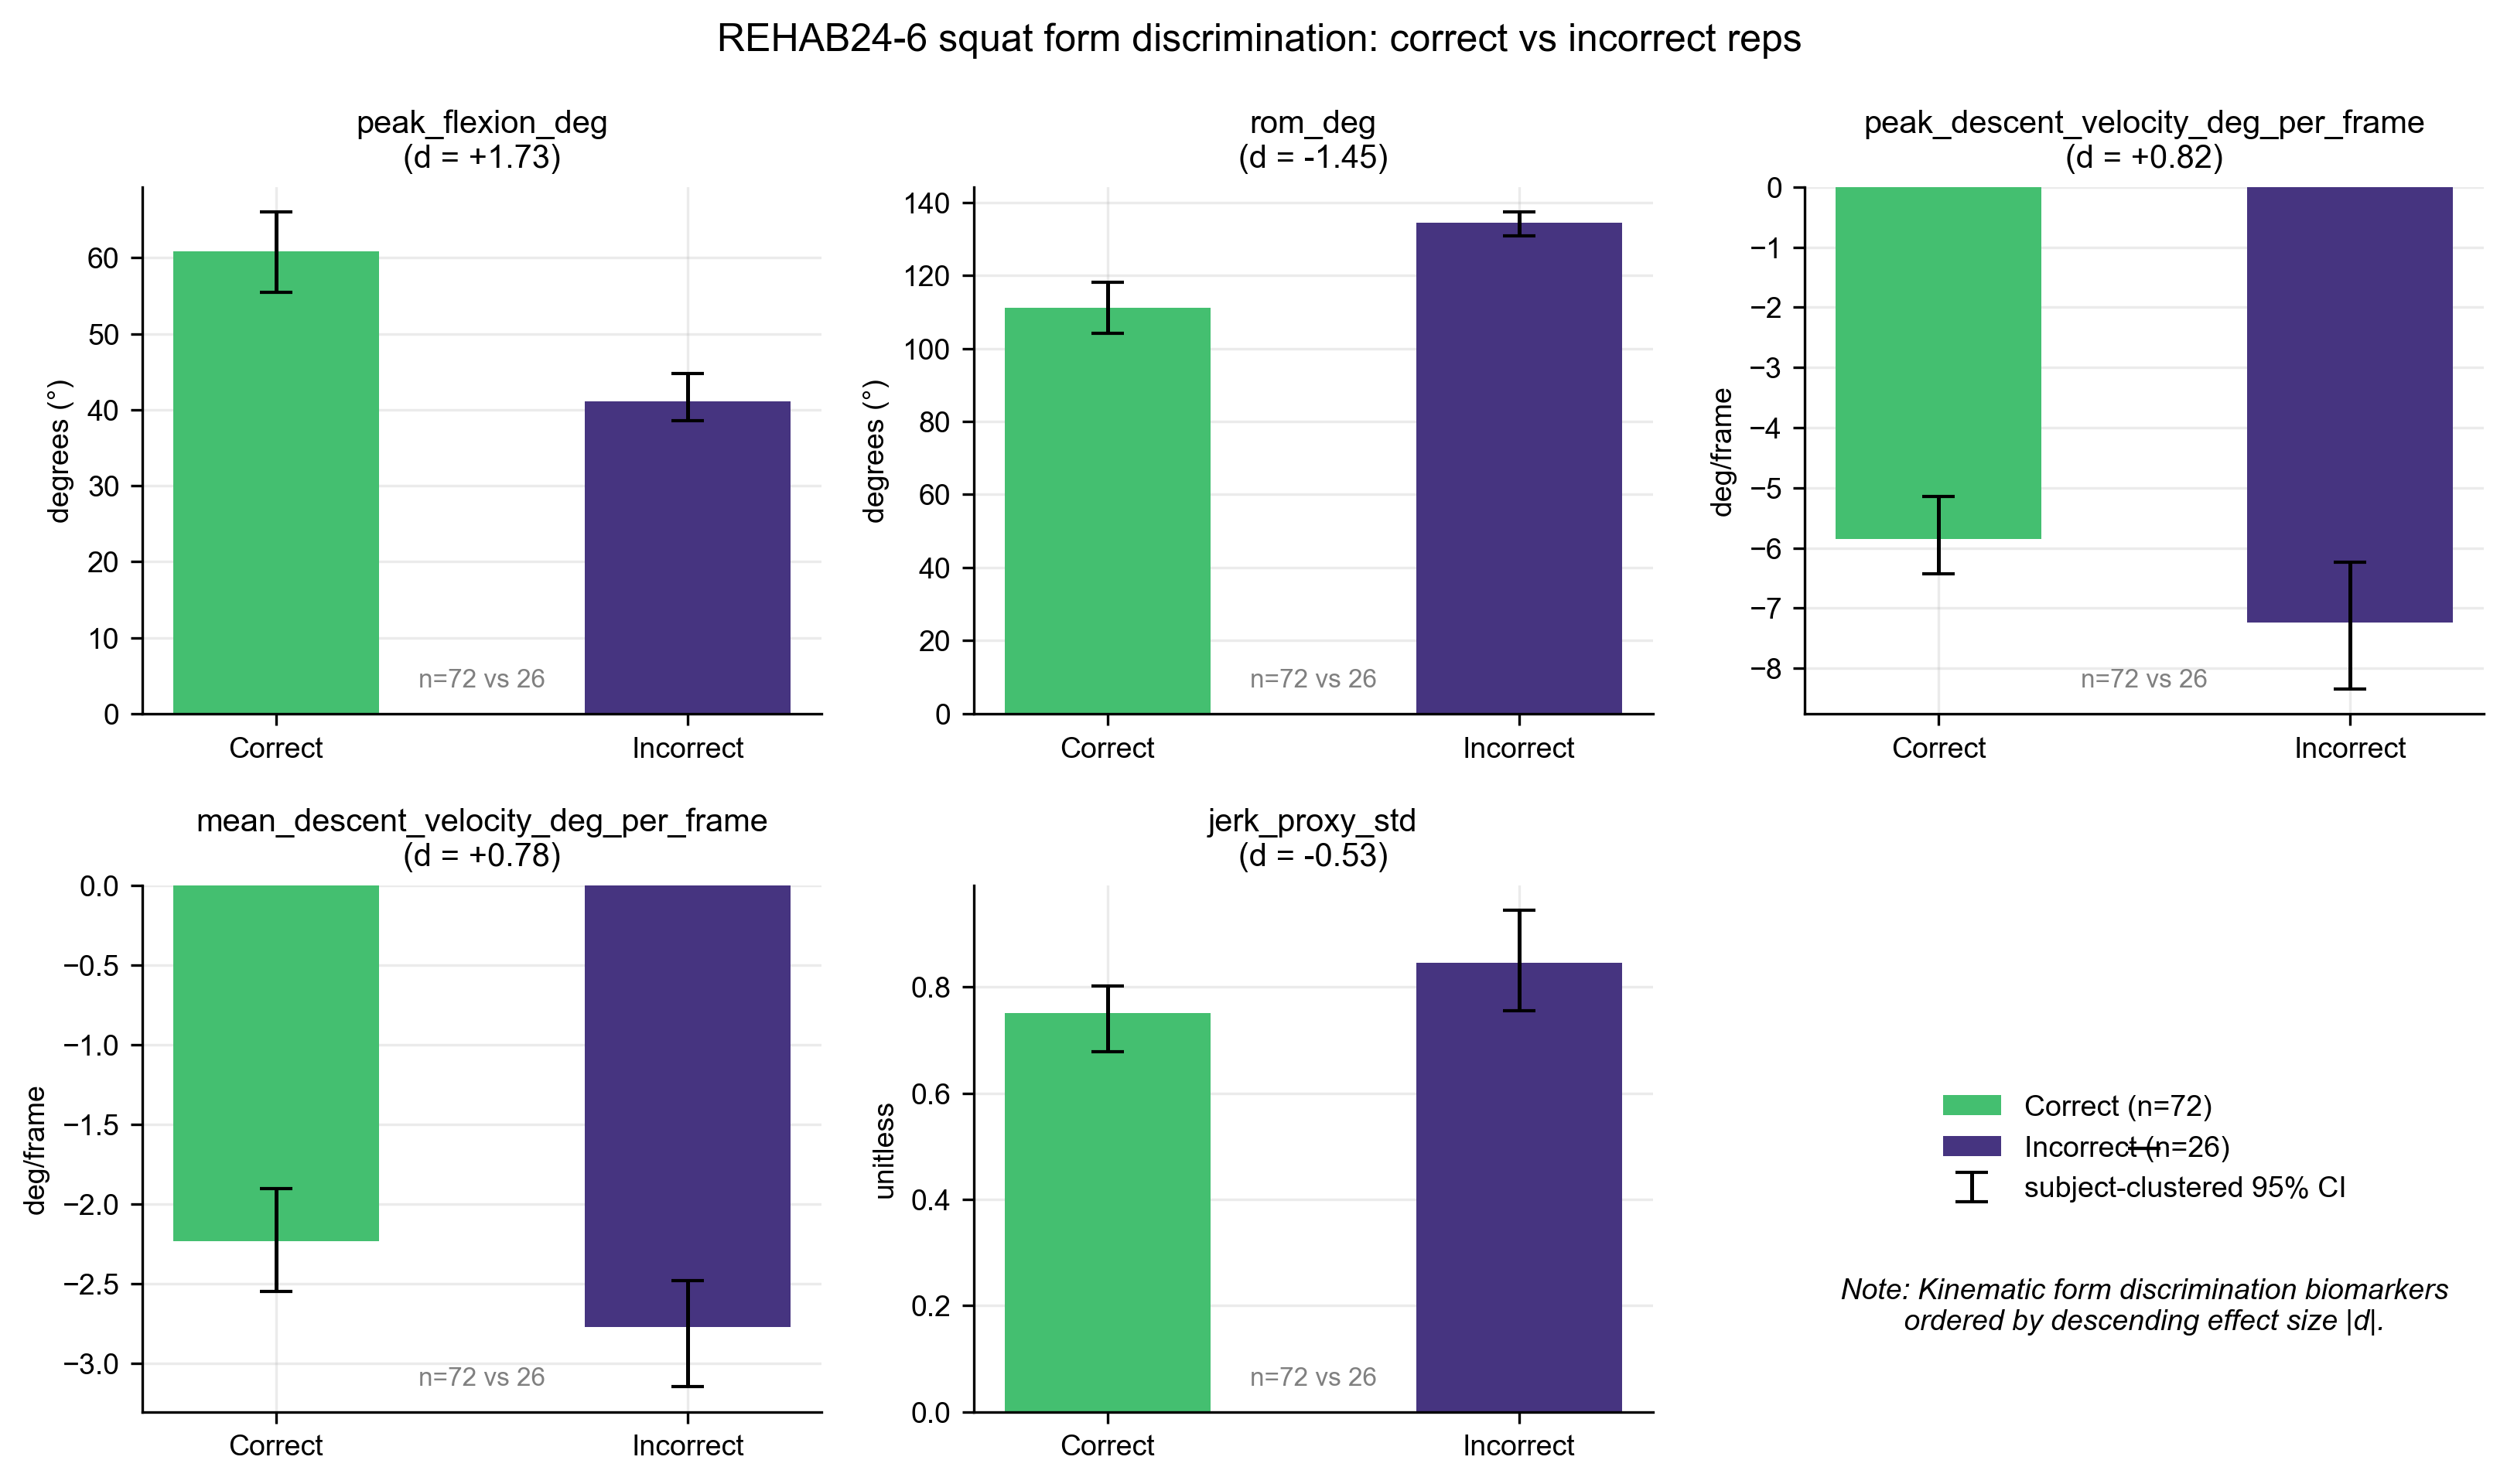
\includegraphics[width=0.92\textwidth]{fig4_1_correct_vs_incorrect.png}
  \caption{Knee Flexion Angle Distributions --- Correct vs.\ Incorrect. Histograms of peak flexion and ROM for correct ($n=72$) and incorrect ($n=26$) squat repetitions, illustrating the deep-flexion shift in incorrect executions.}
  \label{fig:squat-distributions}
\end{figure}

\begin{figure}[htbp]
  \centering
  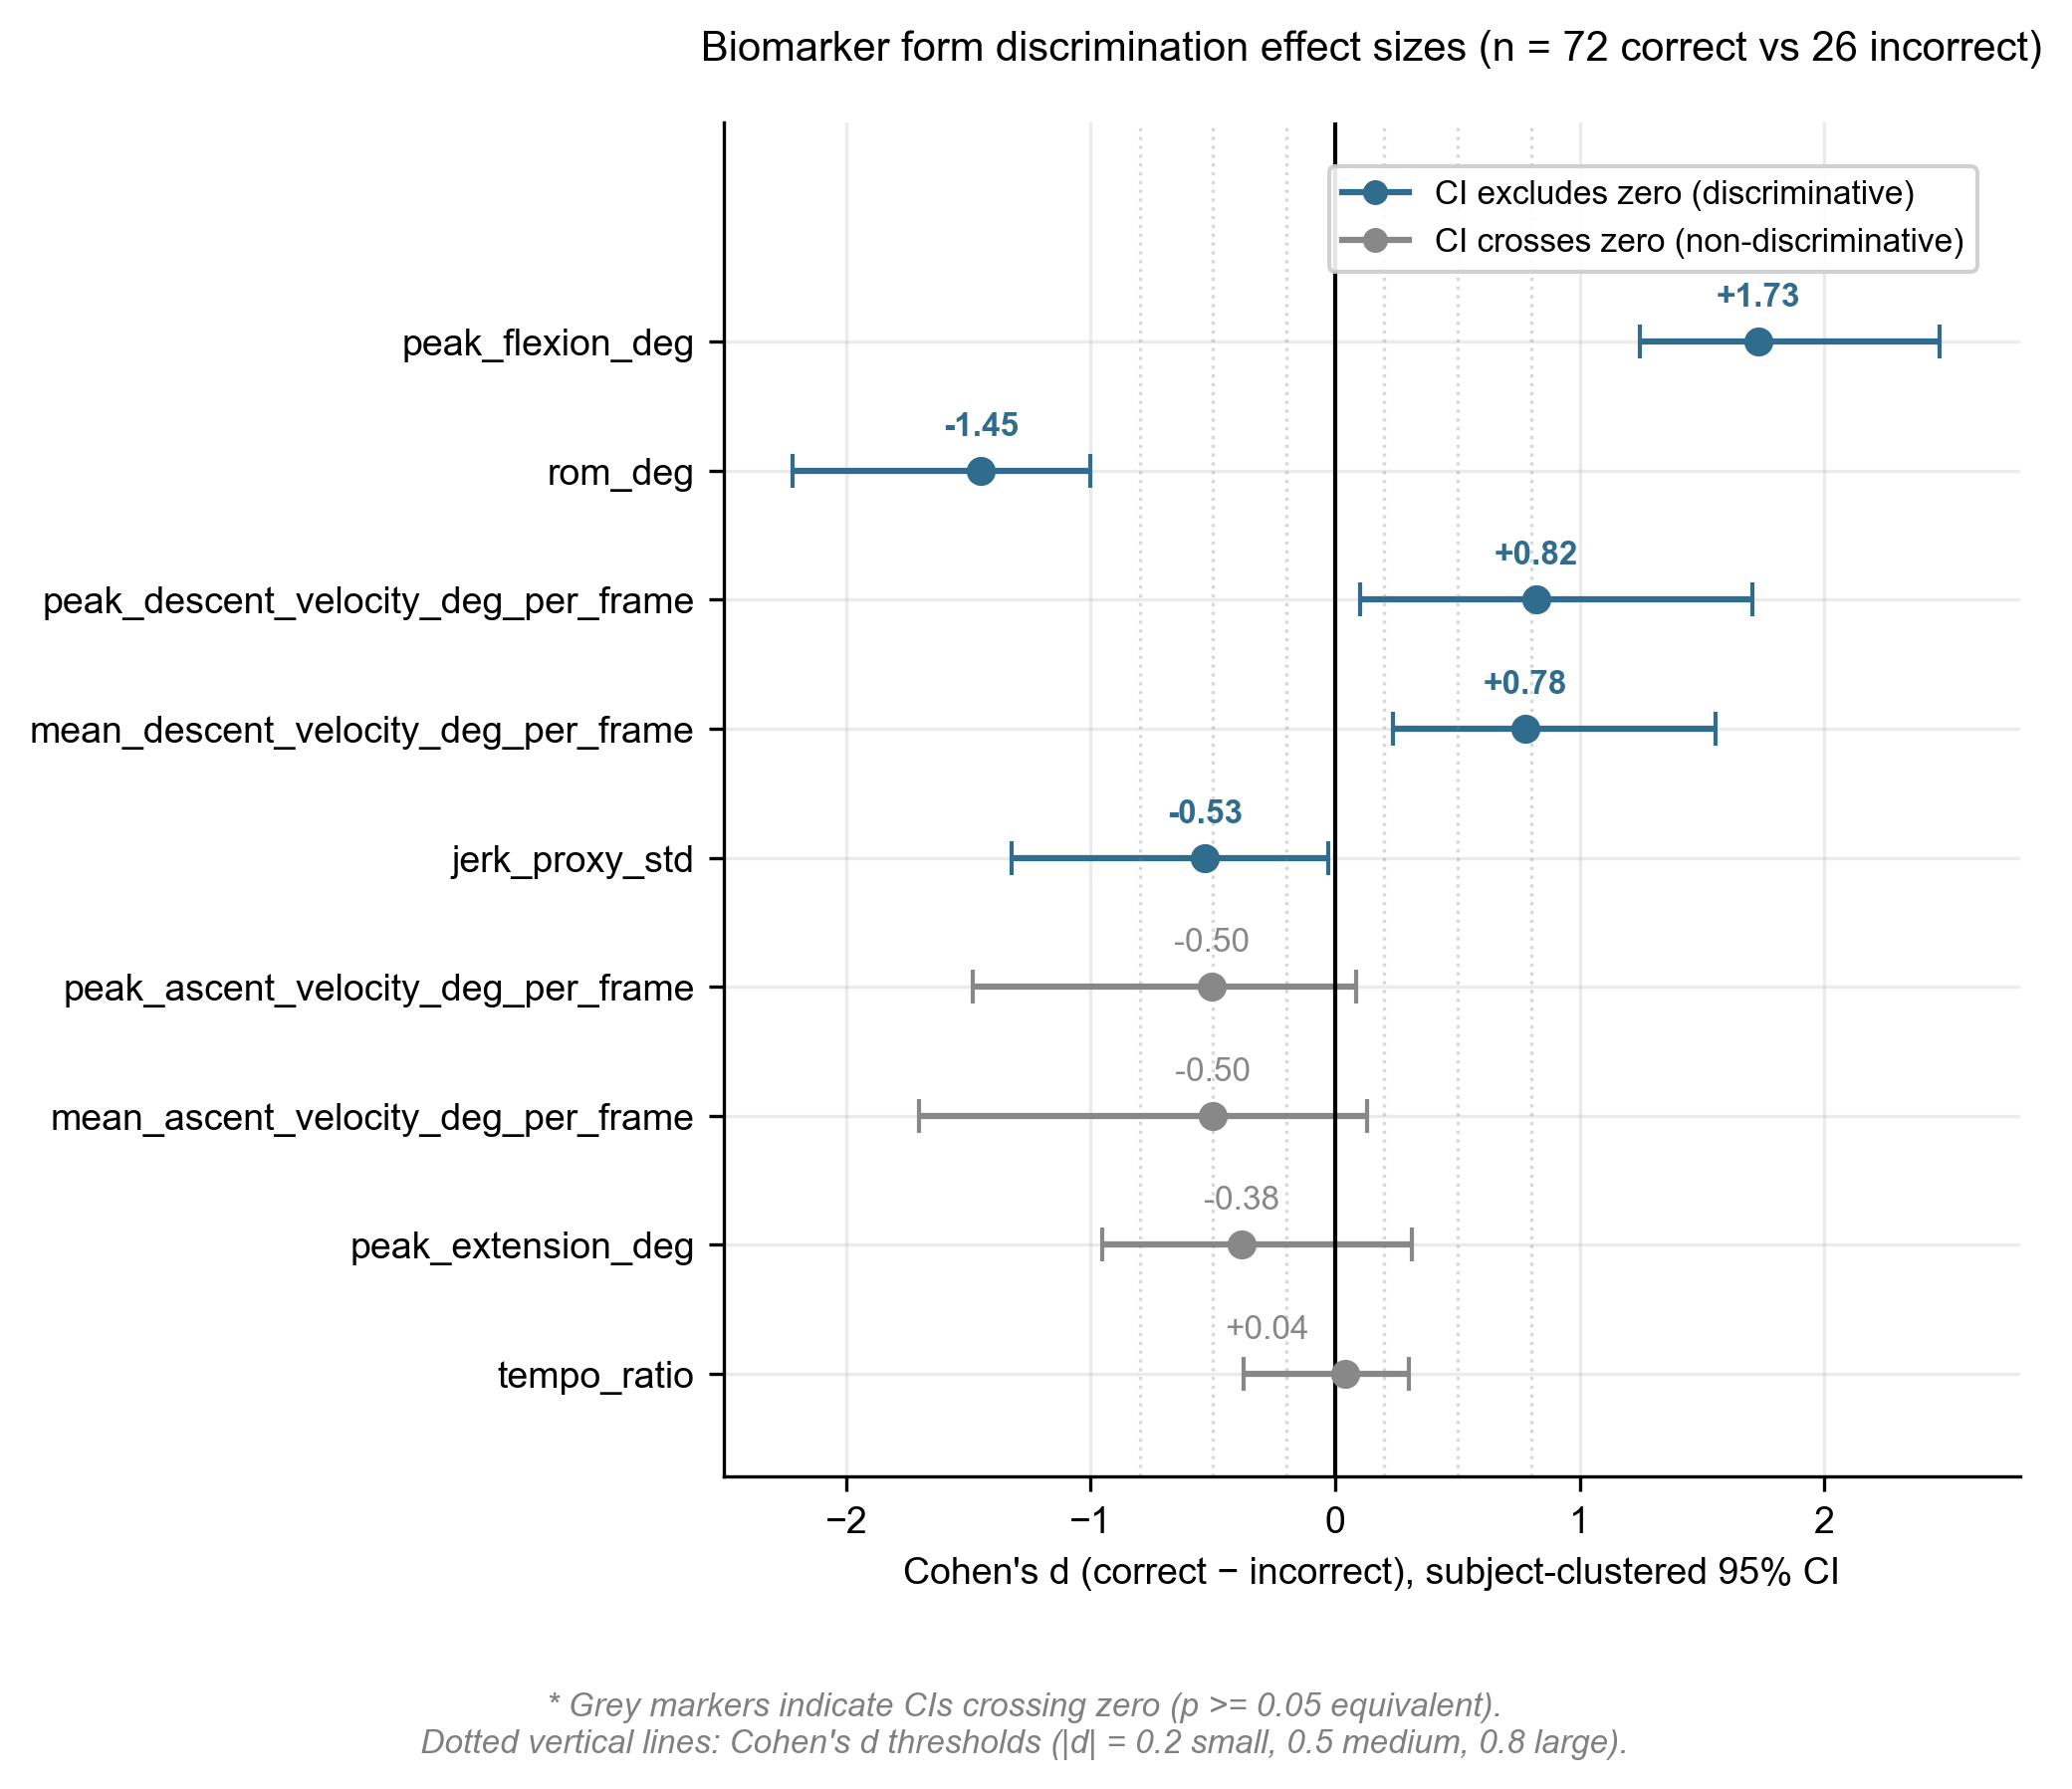
\includegraphics[width=0.92\textwidth]{fig4_2_effect_sizes.png}
  \caption{Forest Plot of Cohen's $d$ Effect Sizes and 95\% Confidence Intervals for all squat biomarkers. Discriminative descent metrics and non-discriminative ascent metrics are clearly separated.}
  \label{fig:squat-effect-sizes}
\end{figure}

\begin{figure}[htbp]
  \centering
  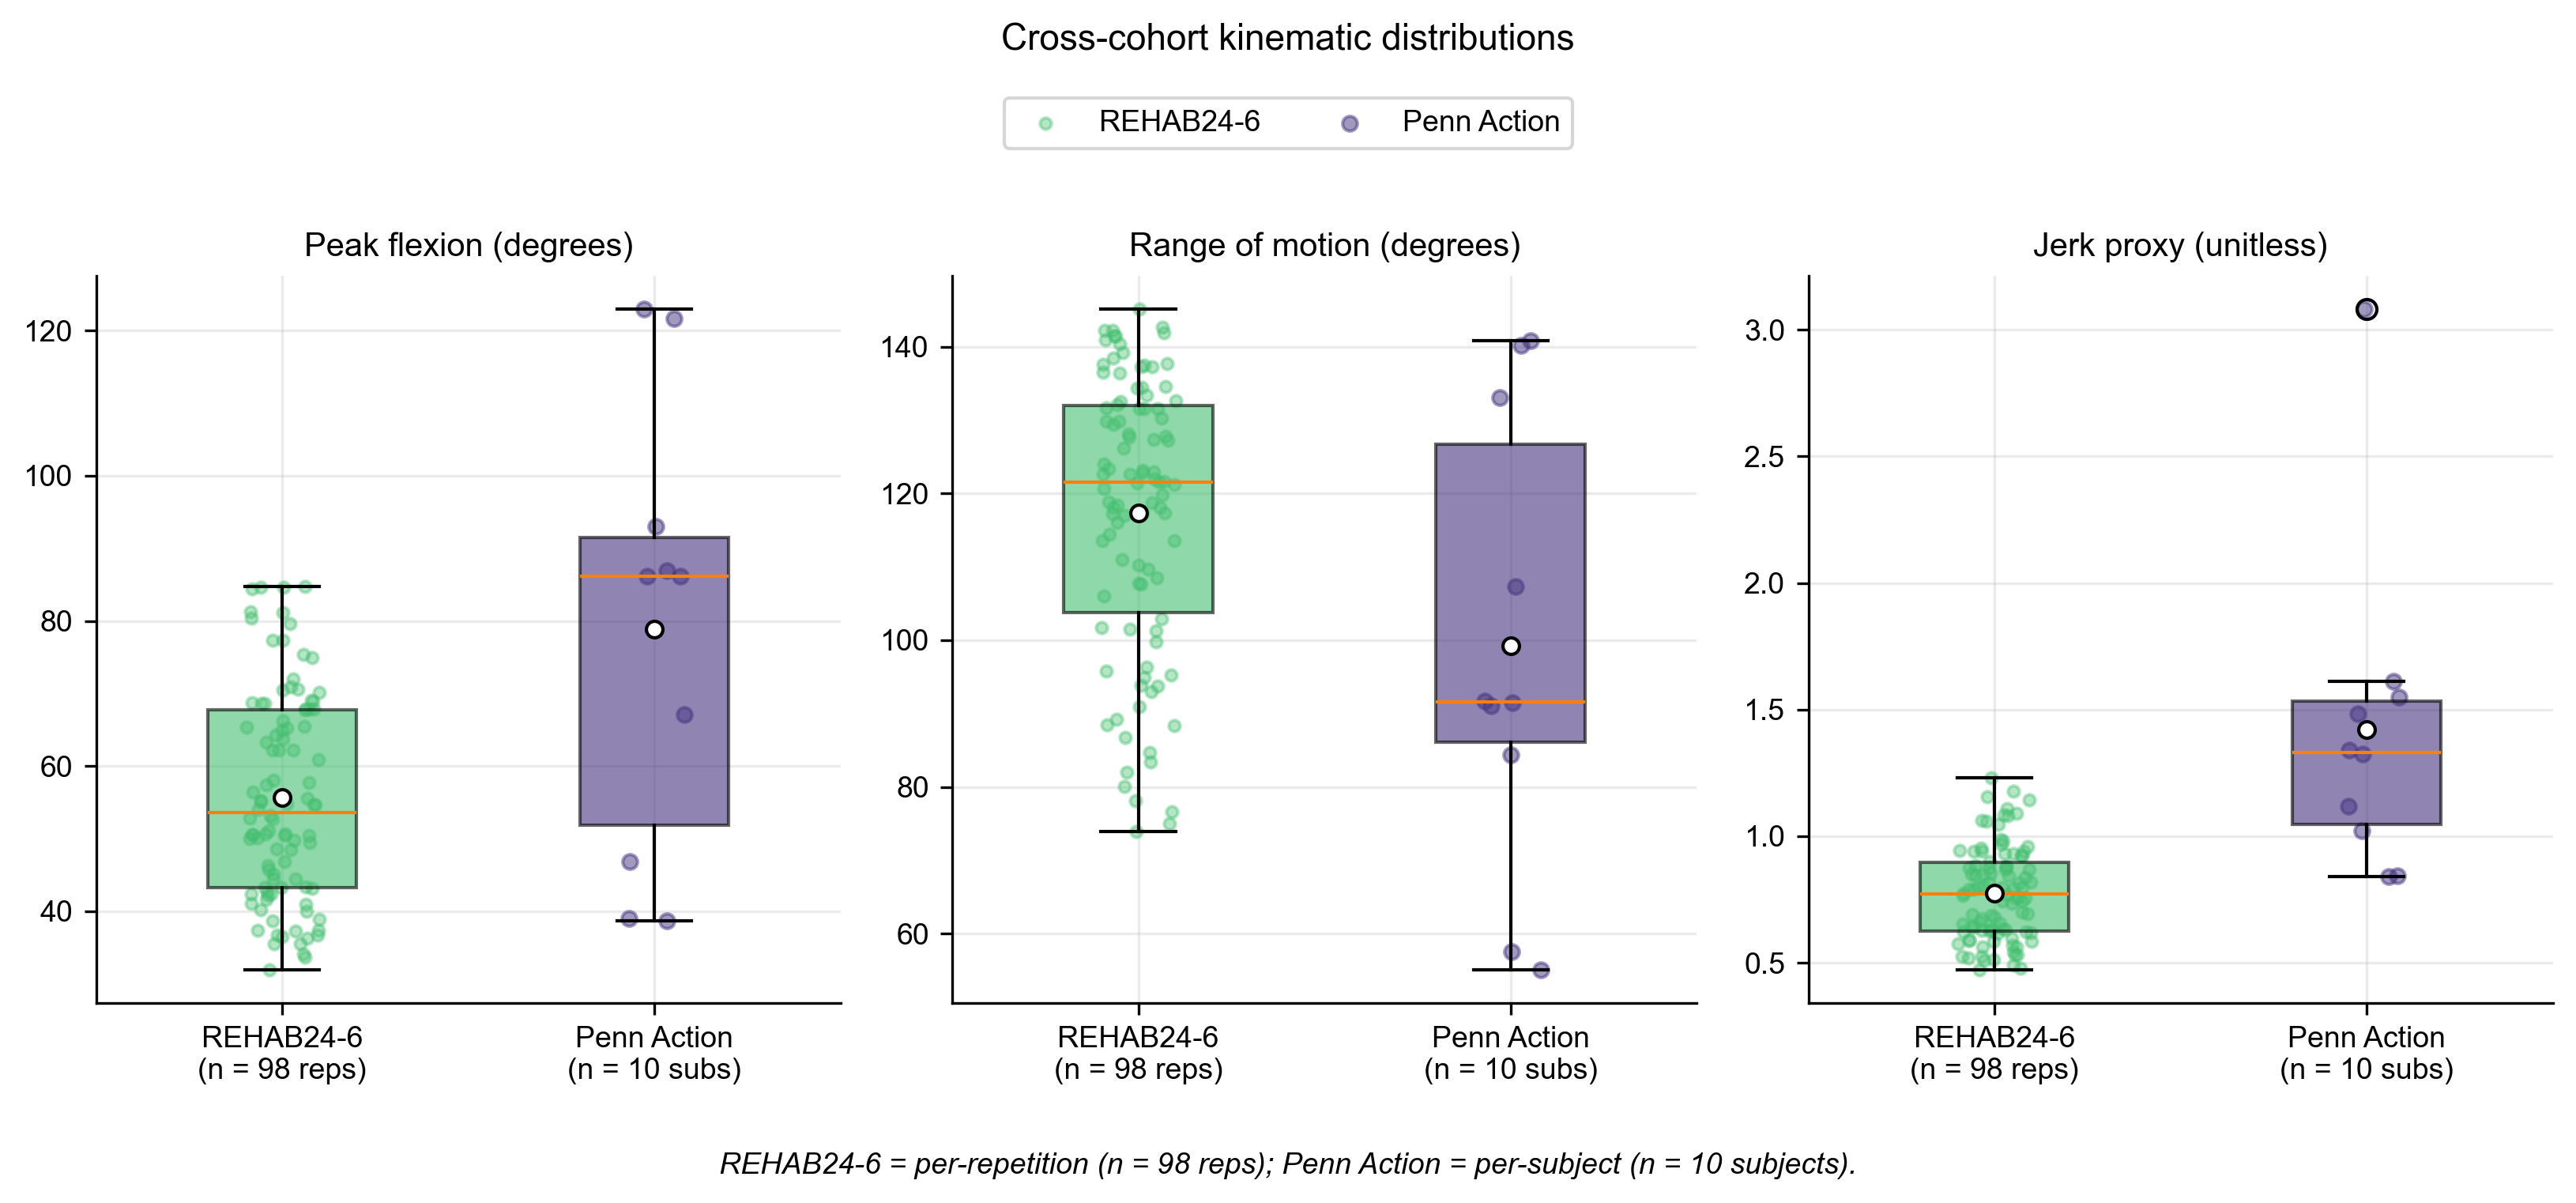
\includegraphics[width=0.92\textwidth]{fig4_3_cross_cohort.png}
  \caption{Cross-Cohort Kinematic Distribution Comparison. Overlay of Penn Action ($n=10$ subjects) \citep{Zhang_Penn_Action_2013} and REHAB24-6 ($n=98$ reps) joint angle distributions, demonstrating biomechanical range generalisation.}
  \label{fig:squat-cross-cohort}
\end{figure}

\begin{figure}[htbp]
  \centering
  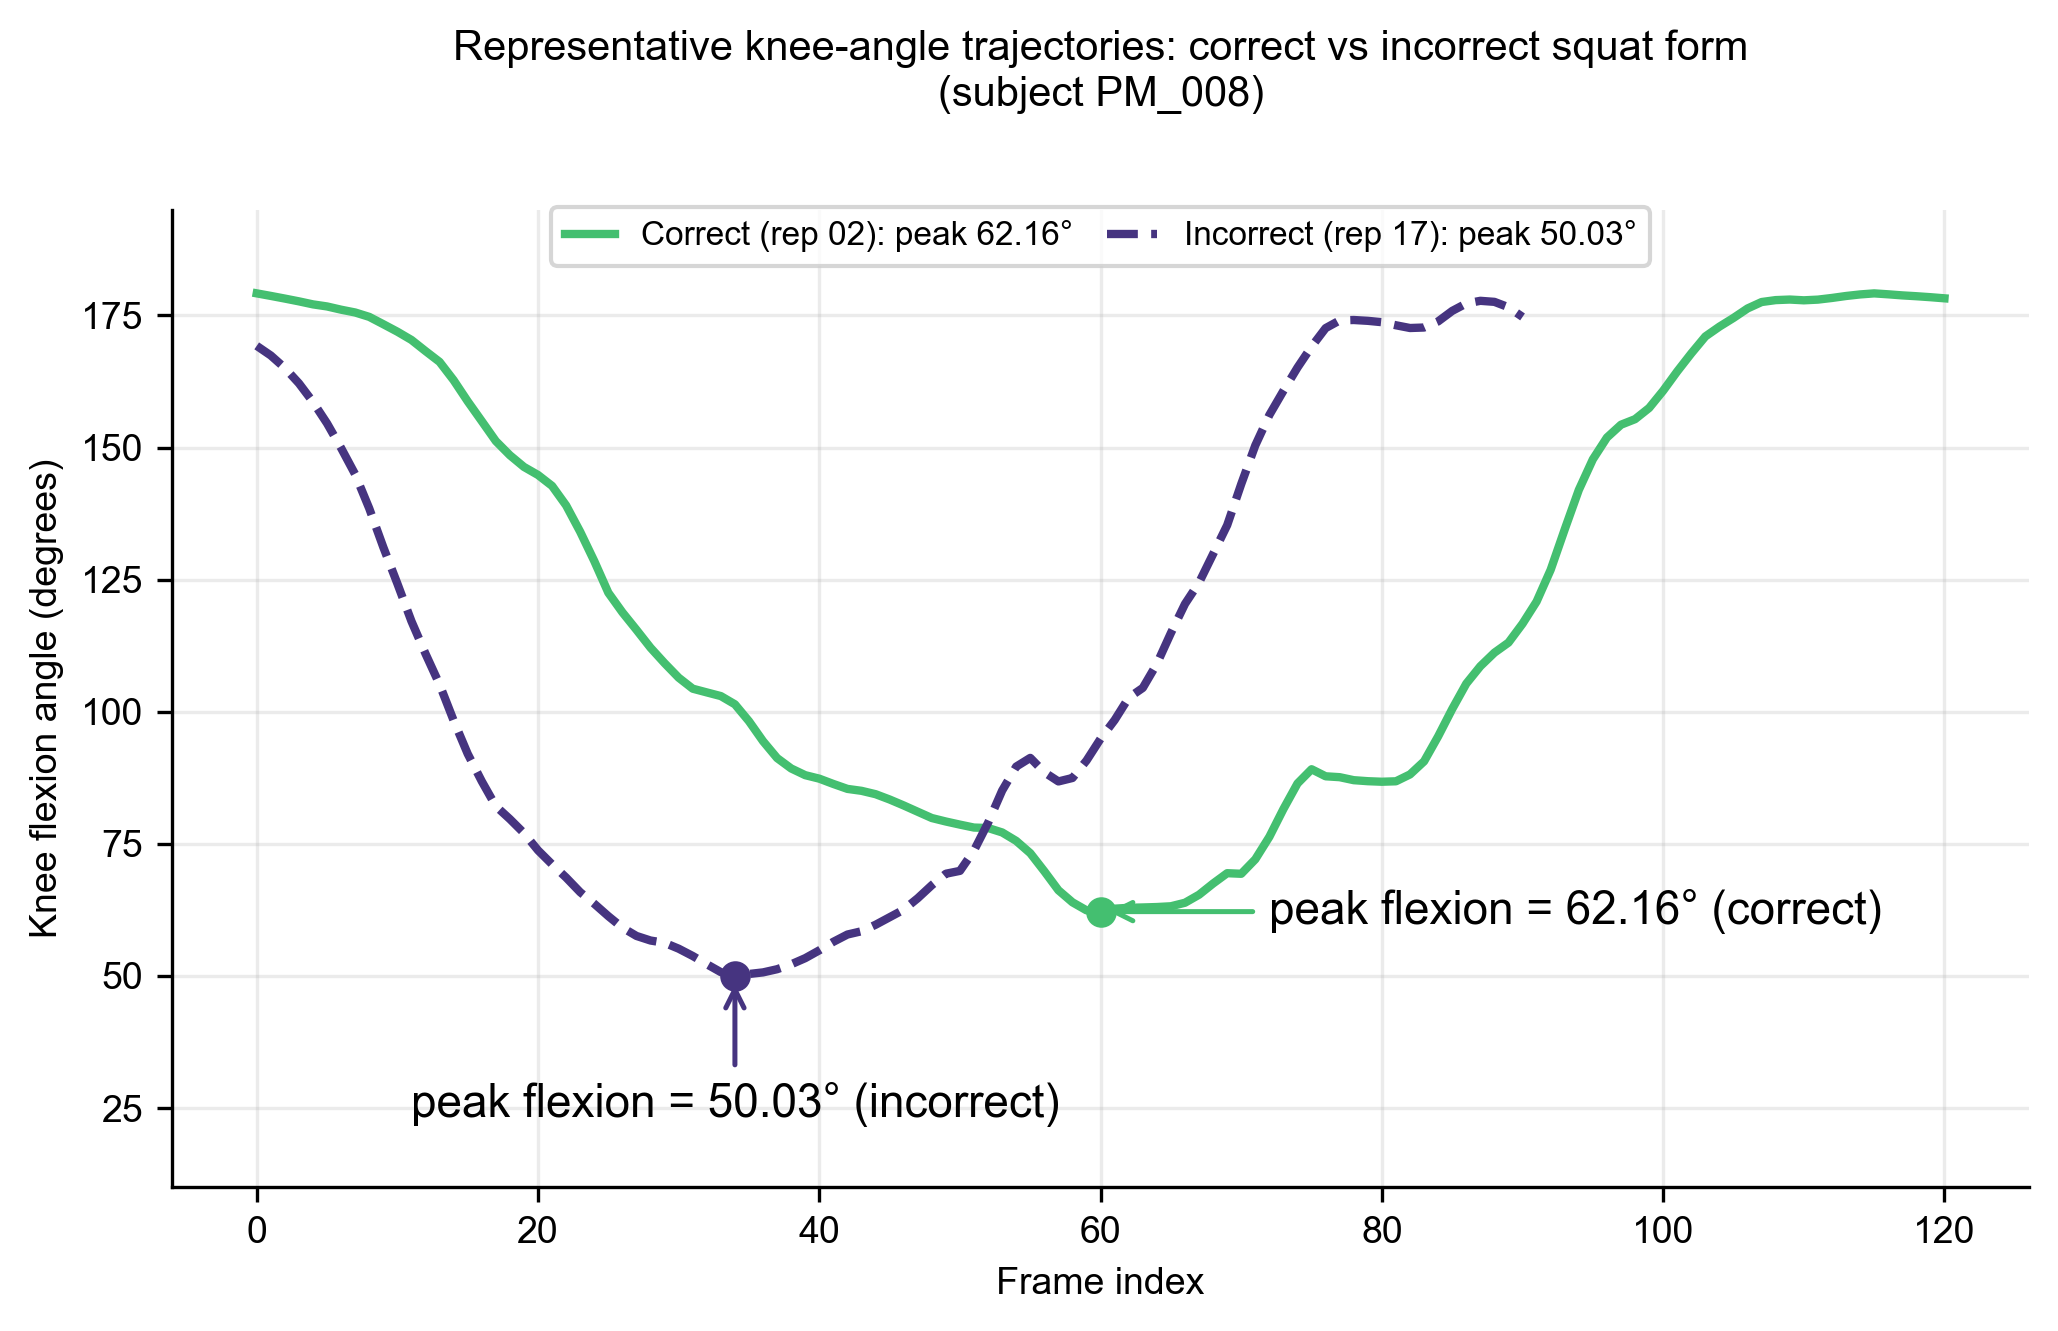
\includegraphics[width=0.92\textwidth]{fig4_4_trajectories.png}
  \caption{Representative Correct vs.\ Incorrect Knee Flexion Trajectories. Time-series overlay of a correct (Subject 1, rep 2, 121 frames) and incorrect (Subject 1, rep 17, 91 frames) squat repetition, illustrating the rapid eccentric descent and excessive depth in the incorrect execution.}
  \label{fig:squat-trajectories}
\end{figure}
\chapter{Unilateral Lunge Kinematic Screening}
\label{ch:lunge}

% SOURCE: results_lunge_v2.md
% STATUS: converted from markdown
% NOTE: [source:] tags stripped per ASSEMBLY_PLAN.md (harvested to appF)


This chapter presents the markerless kinematic screening results for the lunge exercise, evaluating form discrimination under unilateral loading, tracking failure modes arising from asymmetric self-occlusion, and the cross-exercise kinematic divergence between lunge and squat ascent dynamics. Statistical methods follow Chapter 2.



\section{Cohort and Methodological Setup}
\label{sec:5-1-cohort-and-methodological-setup}


Lunges were analyzed using the REHAB24-6 physical therapy dataset, filtering for the lunge exercise (\texttt{exercise\_id == 5}), front-facing orthogonal camera placement (\texttt{cam17\_orientation == 'front'}), and error-free motion capture reference (\texttt{mocap\_erroneous == 0}):

\begin{enumerate}
  \item \textbf{Assembled Cohort}: \textbf{$88$ lunge repetitions} across \textbf{$8$ subjects}.
  \item \textbf{Usable Analytical Cohort}: After quality filtering and phase-identification validation, \textbf{$61$ repetitions} ($25$ correct, $36$ incorrect) across \textbf{$7$ subjects}.
\end{enumerate}

\subsection{Pose-Pipeline Failure Modes and Exclusions}
\label{sec:5-1-1-pose-pipeline-failure-modes-and-exclusions}

Unlike the squat exercise (100\% tracking completion rate in REHAB24-6), the lunge resulted in \textbf{$27$ repetitions ($30.68\%$)} failing the phase-identification validation gate due to tracking loss exceeding 30\% of repetition duration. Failures were concentrated in two subjects:
\begin{itemize}
  \item \textbf{Subject 8 (\texttt{PM\_112})}: $12/12$ repetitions failed ($100.0\%$) — subject dropped entirely.
  \item \textbf{Subject 5 (\texttt{PM\_042})}: $12/13$ repetitions failed ($92.3\%$) — one usable repetition retained.
\end{itemize}

The mechanism is \textbf{contralateral leg self-occlusion}. Because the lunge is an asymmetric exercise, the loaded front leg (\texttt{exercise\_subtype}: \texttt{'front leg left'} or \texttt{'front leg right'}) is frequently occluded by the trailing limb during deep flexion when positioned as the far leg relative to the camera. Unlike the squat, no contralateral fallback is permissible for unilateral screening, so this occlusion causes catastrophic tracking loss.

\subsection{Coordinate Convention}
\label{sec:5-1-2-coordinate-convention}

Consistent with Chapter 4, lunges use the \textbf{included-angle convention} ($\approx 180^\circ$ = standing extension; smaller values = deeper flexion). Subject-clustered bootstrapping (5,000 iterations, subject-level resampling) produces 95\% bootstrap CIs following the procedure described in Chapter 2.



\section{Headline Screening Findings (Form Discrimination)}
\label{sec:5-2-headline-screening-findings-form-discrimination}


Incorrect lunge form was characterized by \textbf{excessive knee flexion depth, a faster descent phase, an elevated jerk profile, and a rapid concentric ascent}. Table 5.1 summarizes the results.


\begin{table}[htbp]
\centering
\scriptsize
\setlength{\tabcolsep}{3pt}
\renewcommand{\arraystretch}{1.2}
\caption{Correct vs. Incorrect Lunge Kinematic Comparison ($n = 61$ reps)}
\label{tab:table-5-1-correct-vs-incorrect-lunge-kinematic-comparison-reps}
\begin{tabular}{@{}p{3.1cm} >{\centering\arraybackslash}p{2.2cm} >{\centering\arraybackslash}p{2.2cm} >{\centering\arraybackslash}p{1.0cm} >{\centering\arraybackslash}p{2.3cm} p{3.4cm}@{}}
\hline
\textbf{Biomarker} & \textbf{Correct Mean} ($n=25$) & \textbf{Incorrect Mean} ($n=36$) & \textbf{Cohen's $d$} & \textbf{95\% CI} & \textbf{Verdict} \\
\hline
Peak Flexion ($^\circ$) & $89.66^\circ \pm 8.33^\circ$ & $68.03^\circ \pm 15.11^\circ$ & $+1.6904$ & $[0.8317, 3.4525]$ & Highly Discriminative \\
ROM ($^\circ$) & $59.02^\circ \pm 20.94^\circ$ & $90.30^\circ \pm 27.00^\circ$ & $-1.2653$ & $[-2.8682, -0.5852]$ & Highly Discriminative \\
Peak Descent Vel. ($^\circ$/fr) & $-2.87^\circ \pm 0.80^\circ$ & $-5.31^\circ \pm 2.68^\circ$ & $+1.1453$ & $[0.7512, 2.0354]$ & Highly Discriminative \\
Mean Descent Vel. ($^\circ$/fr) & $-1.01^\circ \pm 0.28^\circ$ & $-1.75^\circ \pm 0.80^\circ$ & $+1.1563$ & $[0.2863, 2.6316]$ & Highly Discriminative \\
Jerk Proxy SD & $0.46 \pm 0.11$ & $1.07 \pm 0.78$ & $-1.0070$ & $[-1.3663, -0.6526]$ & Highly Discriminative \\
Peak Ascent Vel. ($^\circ$/fr) & $3.85^\circ \pm 1.57^\circ$ & $6.95^\circ \pm 3.93^\circ$ & $-0.9721$ & $[-1.6403, -0.6554]$ & Discriminative \\
Mean Ascent Vel. ($^\circ$/fr) & $1.26^\circ \pm 0.47^\circ$ & $1.87^\circ \pm 0.91^\circ$ & $-0.7962$ & $[-2.0731, -0.0807]$ & Discriminative (Marginal) \\
Peak Extension ($^\circ$) & $148.68^\circ \pm 18.09^\circ$ & $158.33^\circ \pm 20.25^\circ$ & $-0.4972$ & $[-1.7633, 0.1533]$ & Non-Discriminative (CI crosses zero) \\
Tempo Ratio & $0.88 \pm 0.28$ & $1.04 \pm 0.47$ & $-0.3796$ & $[-0.7240, 0.1386]$ & Non-Discriminative (Precise Null) \\
\hline
\end{tabular}
\end{table}

\subsection{Flexion Depth and Joint Excursion}
\label{sec:5-2-1-flexion-depth-and-joint-excursion}

Incorrect lunges reached a mean peak included angle of $\mathbf{68.03^\circ \pm 15.11^\circ}$ versus $\mathbf{89.66^\circ \pm 8.33^\circ}$ for correct repetitions — a large effect ($d = 1.6904$, 95\% CI: $[0.8317, 3.4525]$). The deeper descent directly enlarged joint excursion: incorrect ROM was $\mathbf{90.30^\circ \pm 27.00^\circ}$ versus $\mathbf{59.02^\circ \pm 20.94^\circ}$ for correct repetitions ($d = -1.2653$, 95\% CI: $[-2.8682, -0.5852]$). The negative $d$ is directionally consistent with the included-angle convention and parallels the squat ROM finding ($d = -1.4484$), aligning with the \texttt{EXCESS\_ROM} screening rule.

\subsection{Trajectory Case-Study Verification}
\label{sec:5-2-2-trajectory-case-study-verification}

The cohort-level depth shift is confirmed by Subject 7 (\texttt{PM\_125}) comparing correct repetition 14 (peak flexion $99.87^\circ$, ROM $51.31^\circ$, $110$ frames) versus incorrect repetition 16 (peak flexion $57.04^\circ$, ROM $102.88^\circ$, $111$ frames). This single-subject trajectory comparison confirms the cohort-level shift is not driven by statistical outliers. All 5 subjects contributing both correct and incorrect repetitions (Subjects 2, 4, 6, 7, 9) displayed consistent negative peak flexion shifts ($-24.14^\circ$ to $-29.35^\circ$) and positive ROM shifts ($+24.44^\circ$ to $+52.87^\circ$) during incorrect lunges.

\subsection{Descent Velocity and Jerk}
\label{sec:5-2-3-descent-velocity-and-jerk}

All three descent-phase biomarkers were highly discriminative. Peak descent velocity: correct $-2.87^\circ/\text{frame} \pm 0.80^\circ/\text{frame}$ vs. incorrect $-5.31^\circ/\text{frame} \pm 2.68^\circ/\text{frame}$ ($d = 1.1453$, 95\% CI: $[0.7512, 2.0354]$). Mean descent velocity: correct $-1.01^\circ/\text{frame} \pm 0.28^\circ/\text{frame}$ vs. incorrect $-1.75^\circ/\text{frame} \pm 0.80^\circ/\text{frame}$ ($d = 1.1563$, 95\% CI: $[0.2863, 2.6316]$). Jerk proxy: correct $0.46 \pm 0.11$ vs. incorrect $1.07 \pm 0.78$ ($d = -1.0070$, 95\% CI: $[-1.3663, -0.6526]$). Positive descent $d$ values reflect physically slower correct-group descent; the negative jerk $d$ indicates smoother correct repetitions.



\section{Cross-Exercise Divergence (The Distinctive Ascent Finding)}
\label{sec:5-3-cross-exercise-divergence-the-distinctive-ascent-finding}


A major finding of this multi-exercise evaluation is the behavior of the concentric ascent phase, which reveals a distinct biomechanical divergence between squats and lunges.

\subsection{Ascent Velocity Discrimination in Lunges}
\label{sec:5-3-1-ascent-velocity-discrimination-in-lunges}

Unlike squats — where both ascent velocity metrics had confidence intervals crossing zero and were non-discriminative — \textbf{both ascent velocity biomarkers discriminated lunge execution quality} with confidence intervals that exclude zero:
\begin{itemize}
  \item \textbf{Peak Ascent Velocity}: correct $3.85^\circ/\text{frame} \pm 1.57^\circ/\text{frame}$ vs. incorrect $6.95^\circ/\text{frame} \pm 3.93^\circ/\text{frame}$ ($d = -0.9721$, 95\% CI: $[-1.6403, -0.6554]$).
  \item \textbf{Mean Ascent Velocity}: correct $1.26^\circ/\text{frame} \pm 0.47^\circ/\text{frame}$ vs. incorrect $1.87^\circ/\text{frame} \pm 0.91^\circ/\text{frame}$ ($d = -0.7962$, 95\% CI: $[-2.0731, -0.0807]$).
\end{itemize}

The negative Cohen's $d$ values reflect that correct lunges exhibited slower (smaller) ascent velocities than incorrect lunges. Mean ascent velocity is classified as \textbf{Discriminative (Marginal)} because its CI upper bound approaches zero ($-0.0807$), but the interval excludes zero, confirming reliability.

\subsection{Explicit Contrast with Squat Kinematics and Biomechanical Explanation}
\label{sec:5-3-2-explicit-contrast-with-squat-kinematics-and-biomechanical-explanation}

In the squat cohort, peak ascent velocity ($d = -0.5049$, 95\% CI: $[-1.4838, +0.0848]$) and mean ascent velocity ($d = -0.4996$, 95\% CI: $[-1.7017, +0.1301]$) both crossed zero — non-discriminative. In the lunge cohort, both were discriminative. This divergence has a clear biomechanical basis: the squat is bilateral, with body mass supported symmetrically, allowing a controlled concentric ascent. The lunge is an asymmetric unilateral propulsion task — from an excessively deep bottom position, the subject must generate a forceful concentric push-off from the front leg alone to recover standing balance. This rapid spring-back propulsion is a direct kinematic consequence of the deeper, more biomechanically disadvantaged bottom position, and represents an additional form-deviation indicator absent in bilateral squats.

\subsection{Statistical Nulls and Rigor Guardrails}
\label{sec:5-3-3-statistical-nulls-and-rigor-guardrails}

Two biomarkers were non-discriminative: \texttt{peak\_extension\_deg} ($d = -0.4972$, 95\% CI: $[-1.7633, 0.1533]$) and \texttt{tempo\_ratio} ($d = -0.3796$, 95\% CI: $[-0.7240, 0.1386]$), both crossing zero. The \texttt{tempo\_ratio} represents a precise null: relative descent-to-ascent timing remains constant even as absolute speeds diverge.



\section{Discussion and Clinical Screening Guardrails}
\label{sec:5-4-discussion-and-clinical-screening-guardrails}


\subsection{Clinical Interpretation of Depth and Ascent Faults}
\label{sec:5-4-1-clinical-interpretation-of-depth-and-ascent-faults}

Excessive lunge depth increases patellofemoral compressive force and tibiofemoral shear stress beyond the parallel position. The rapid concentric ascent observed in incorrect repetitions represents a dynamic compensation: when joint stability is compromised at deep flexion, subjects rely on a forceful spring-back to recover standing balance. This rapid loading-and-unloading pattern amplifies joint shear stress and is associated with patellofemoral irritation \citep{Powers_2003}.

\subsection{Screening-not-Prediction Framing}
\label{sec:5-4-2-screening-not-prediction-framing}

As established in Chapter 4, this framework is a \textbf{kinematic screening layer} that identifies deviations from a subject's baseline movement template. It does not diagnose clinical pathology or predict injury probability; it flags kinematic patterns biomechanically associated with elevated risk per published literature.



\section{Limitations}
\label{sec:5-5-limitations}


\begin{enumerate}
  \item \textbf{Occlusion Exclusions}: Subject 8 ($12/12$ reps failed) and Subject 5 ($12/13$ reps failed) were excluded due to contralateral self-occlusion, representing a systematic monocular tracking limitation for asymmetric movements.
  \item \textbf{Small Cohort Size}: Only $n = 61$ repetitions across $7$ subjects; reported effect sizes should not be generalized to broader populations.
  \item \textbf{No Cross-Cohort Validation}: Unlike the squat chapter, which compared the lab-based cohort to an in-the-wild Penn Action cohort \citep{Zhang_Penn_Action_2013}, the lunge evaluation was restricted to the REHAB24-6 dataset. No Penn Action-equivalent check was performed for lunges, representing an asymmetry in validation depth.
  \item \textbf{Sagittal-Plane Restriction}: Monocular tracking is blind to frontal-plane errors — knee valgus and pelvic drop — which are heavily associated with ACL injury risk.
\end{enumerate}



\section{Figures and Provenance}
\label{sec:5-6-figures}
The following publication-ready figures support this chapter.

\begin{figure}[htbp]
  \centering
  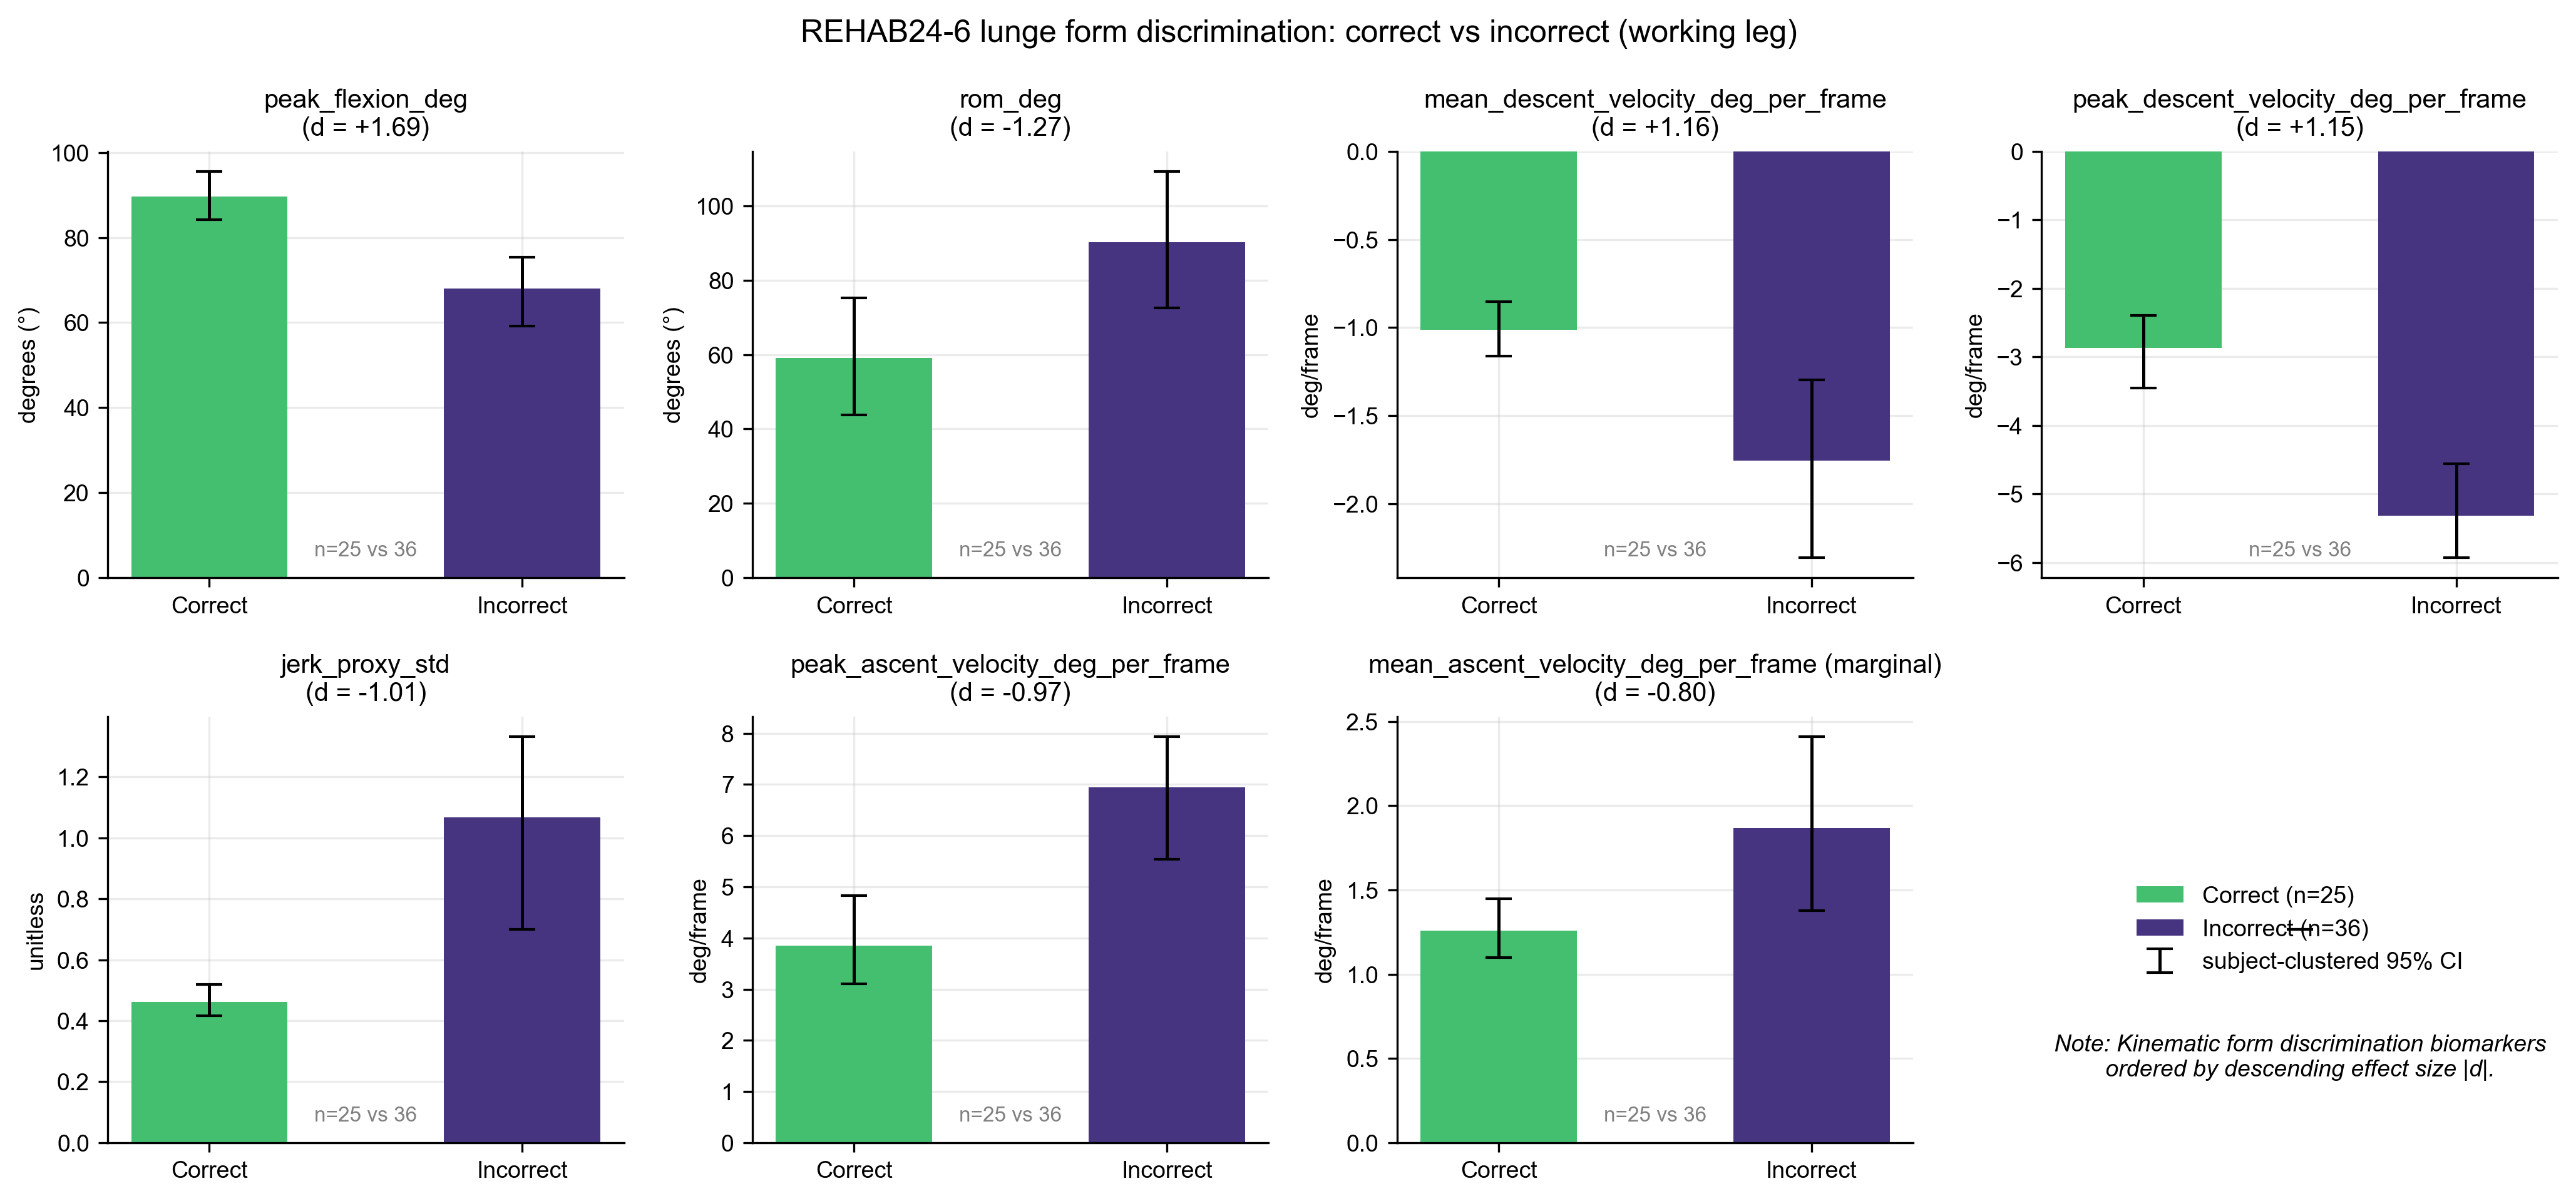
\includegraphics[width=0.92\textwidth]{fig5_1_correct_vs_incorrect.png}
  \caption{Lunge Biomarker Form Discrimination --- Correct vs.\ Incorrect. Multi-panel comparison of peak flexion, ROM, descent/ascent velocity, jerk proxy SD, and related biomarkers for correct ($n = 25$) and incorrect ($n = 36$) lunge repetitions across the REHAB24-6 cohort.}
  \label{fig:lunge-distributions}
\end{figure}

\begin{figure}[htbp]
  \centering
  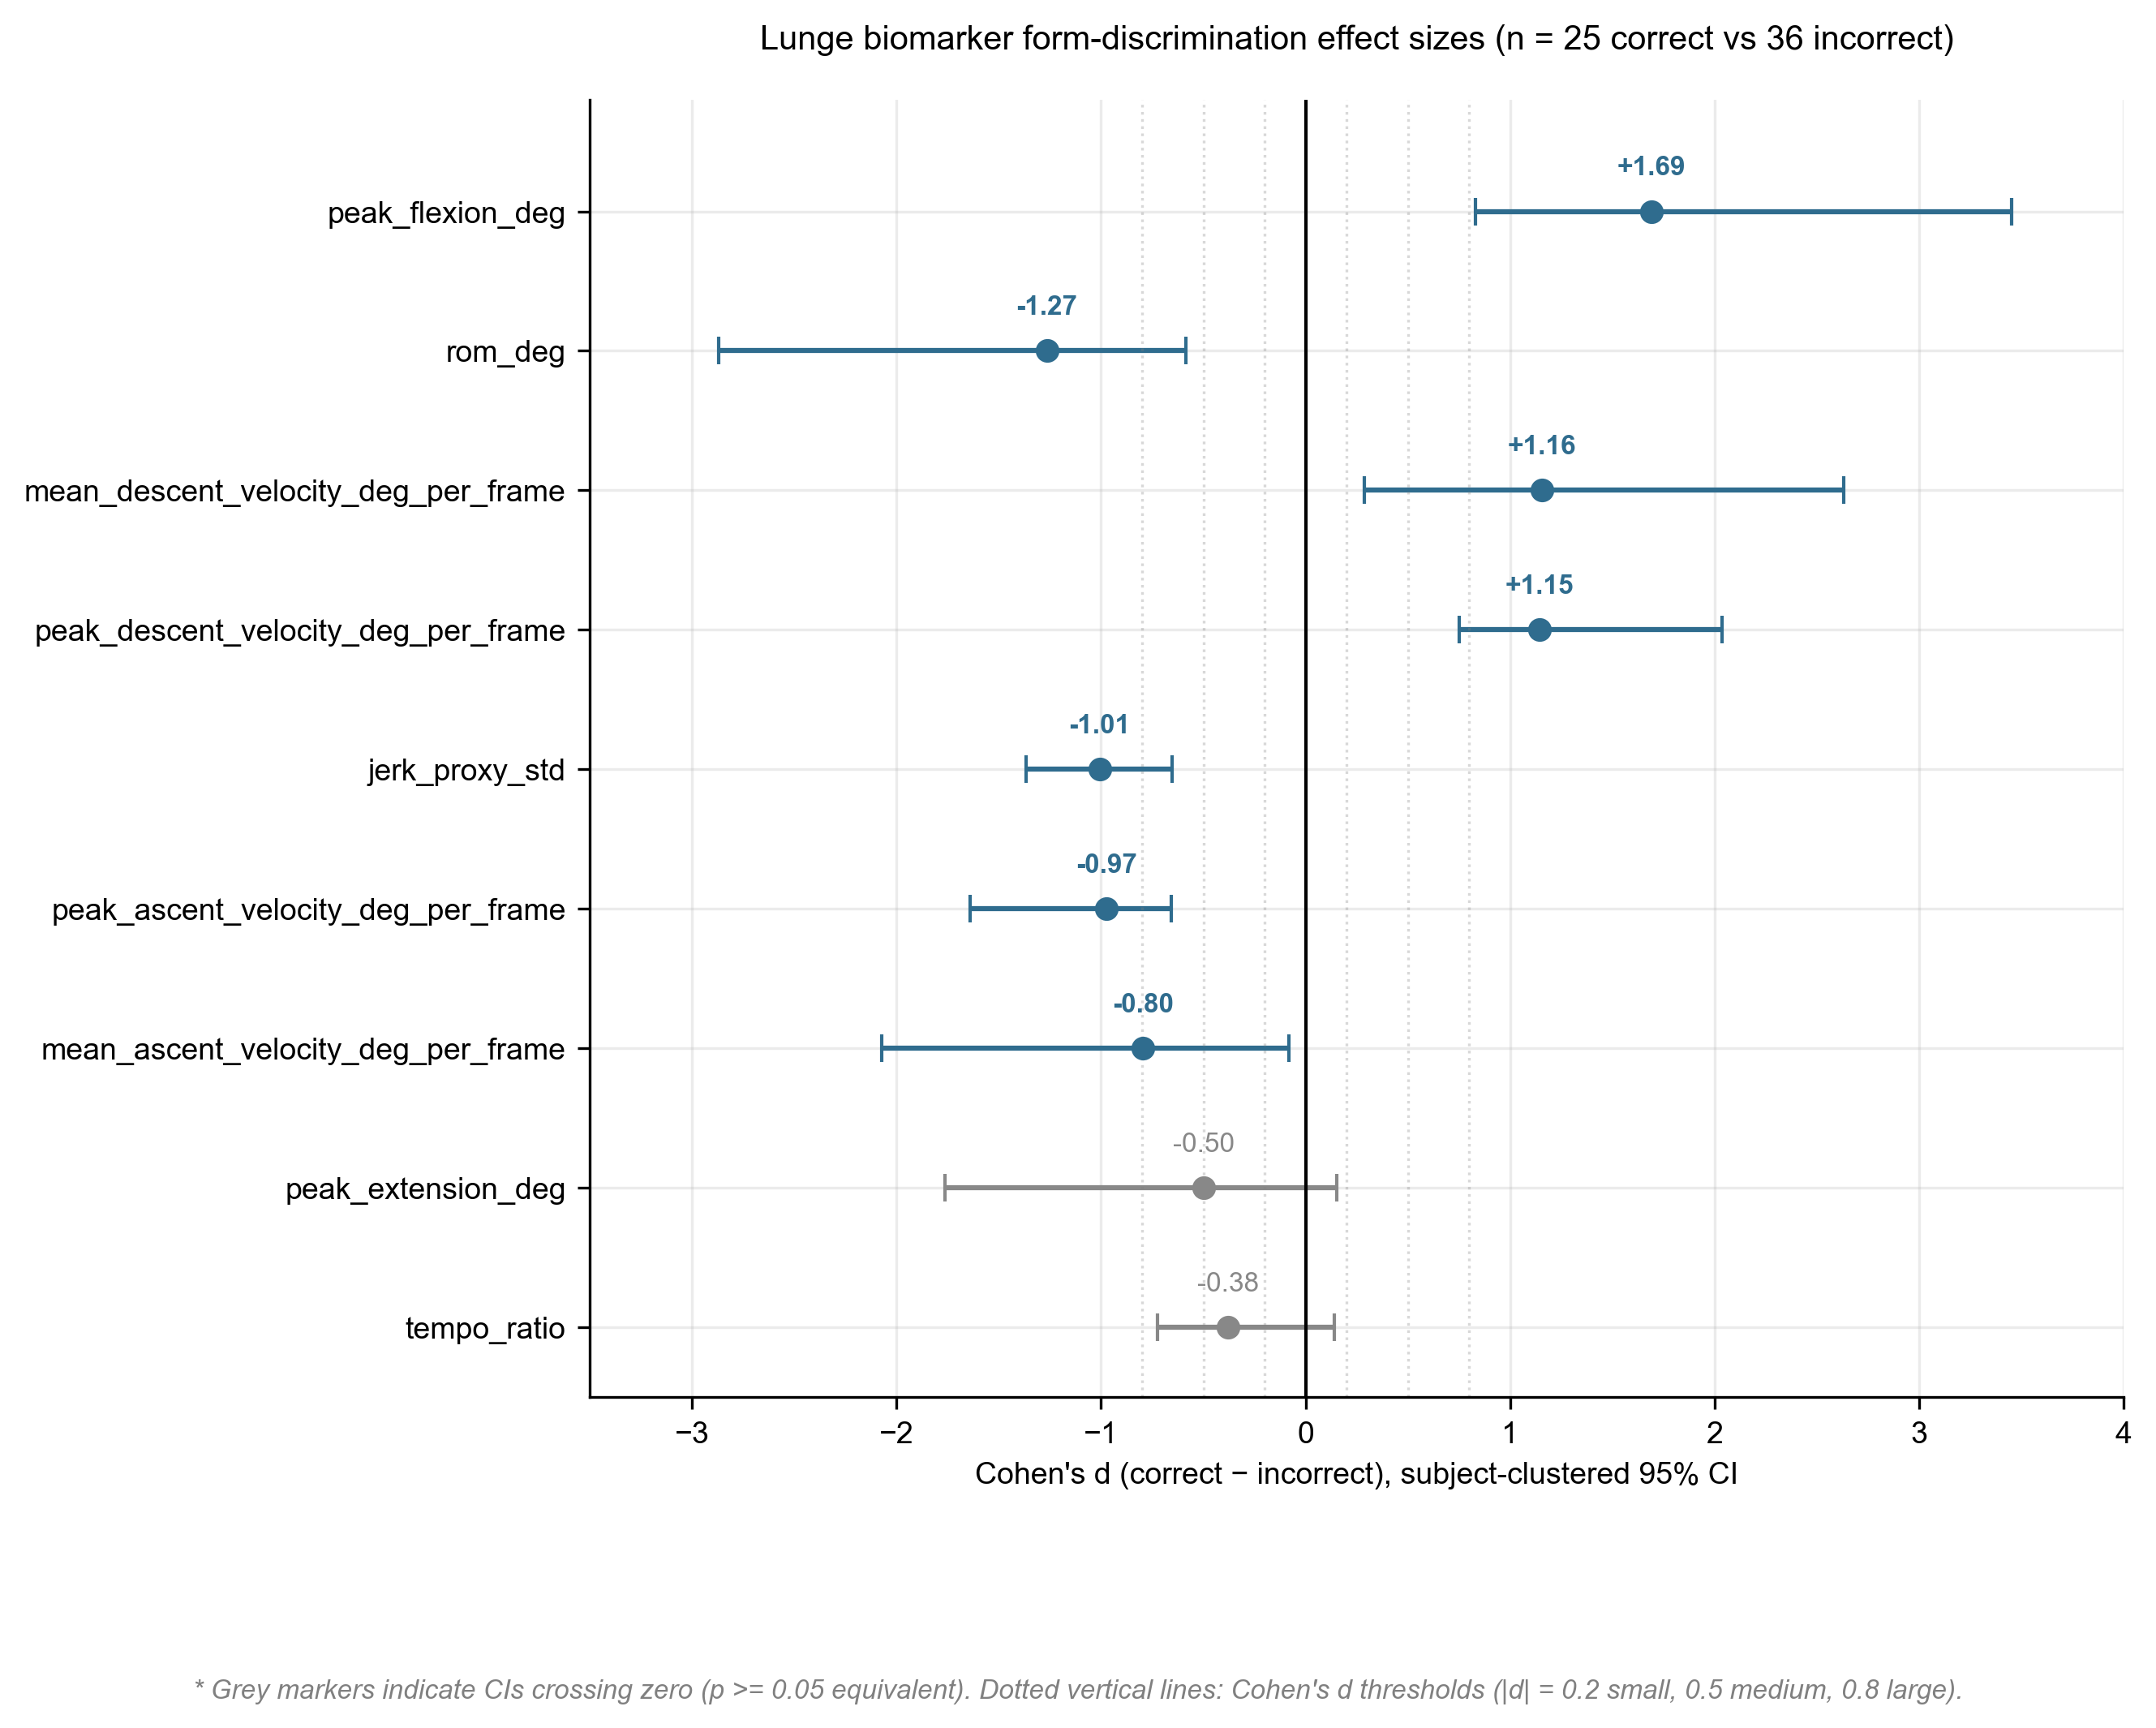
\includegraphics[width=0.92\textwidth]{fig5_2_effect_sizes.png}
  \caption{Forest Plot of Cohen's $d$ Effect Sizes and 95\% Confidence Intervals for all lunge biomarkers. Flexion depth and ascent velocity show strong discriminative power.}
  \label{fig:lunge-effect-sizes}
\end{figure}

\begin{figure}[htbp]
  \centering
  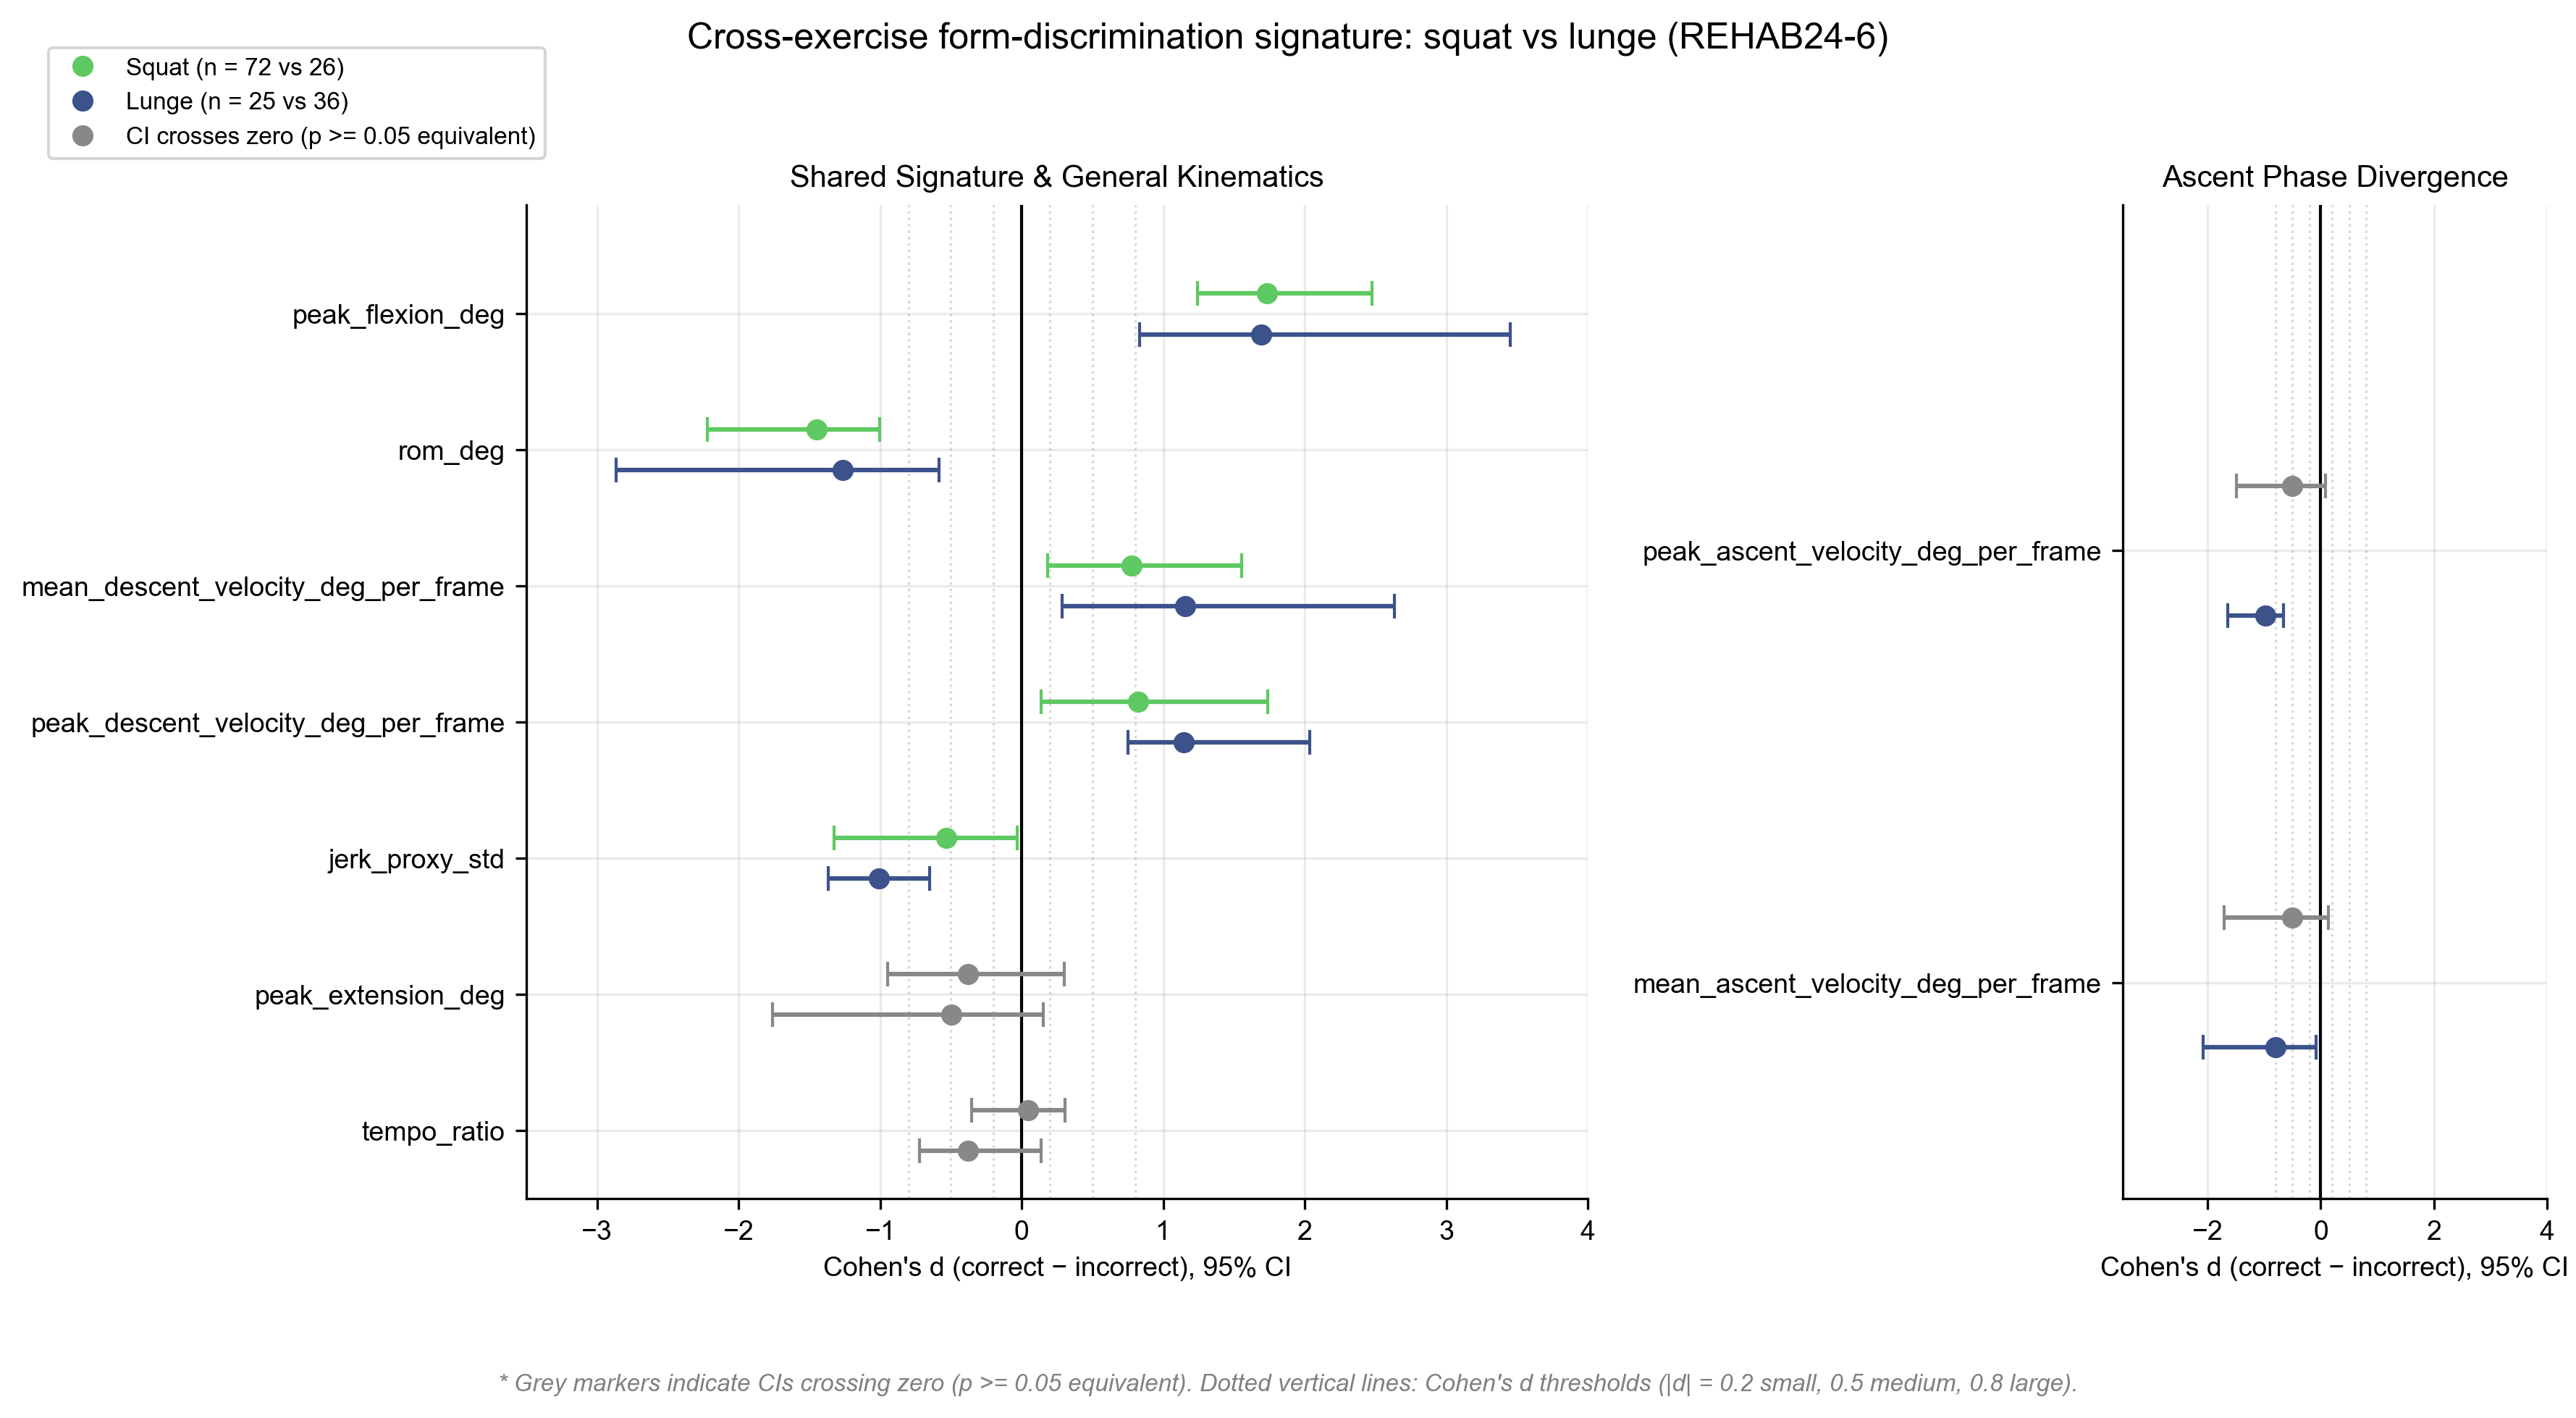
\includegraphics[width=0.92\textwidth]{fig5_3_cross_exercise.png}
  \caption{Cross-Exercise Biomarker Effect-Size Comparison. Squat and lunge Cohen's $d$ effect sizes and 95\% confidence intervals, highlighting task-specific kinematic signatures and exercise-level generalisation.}
  \label{fig:lunge-cross-exercise}
\end{figure}

\begin{figure}[htbp]
  \centering
  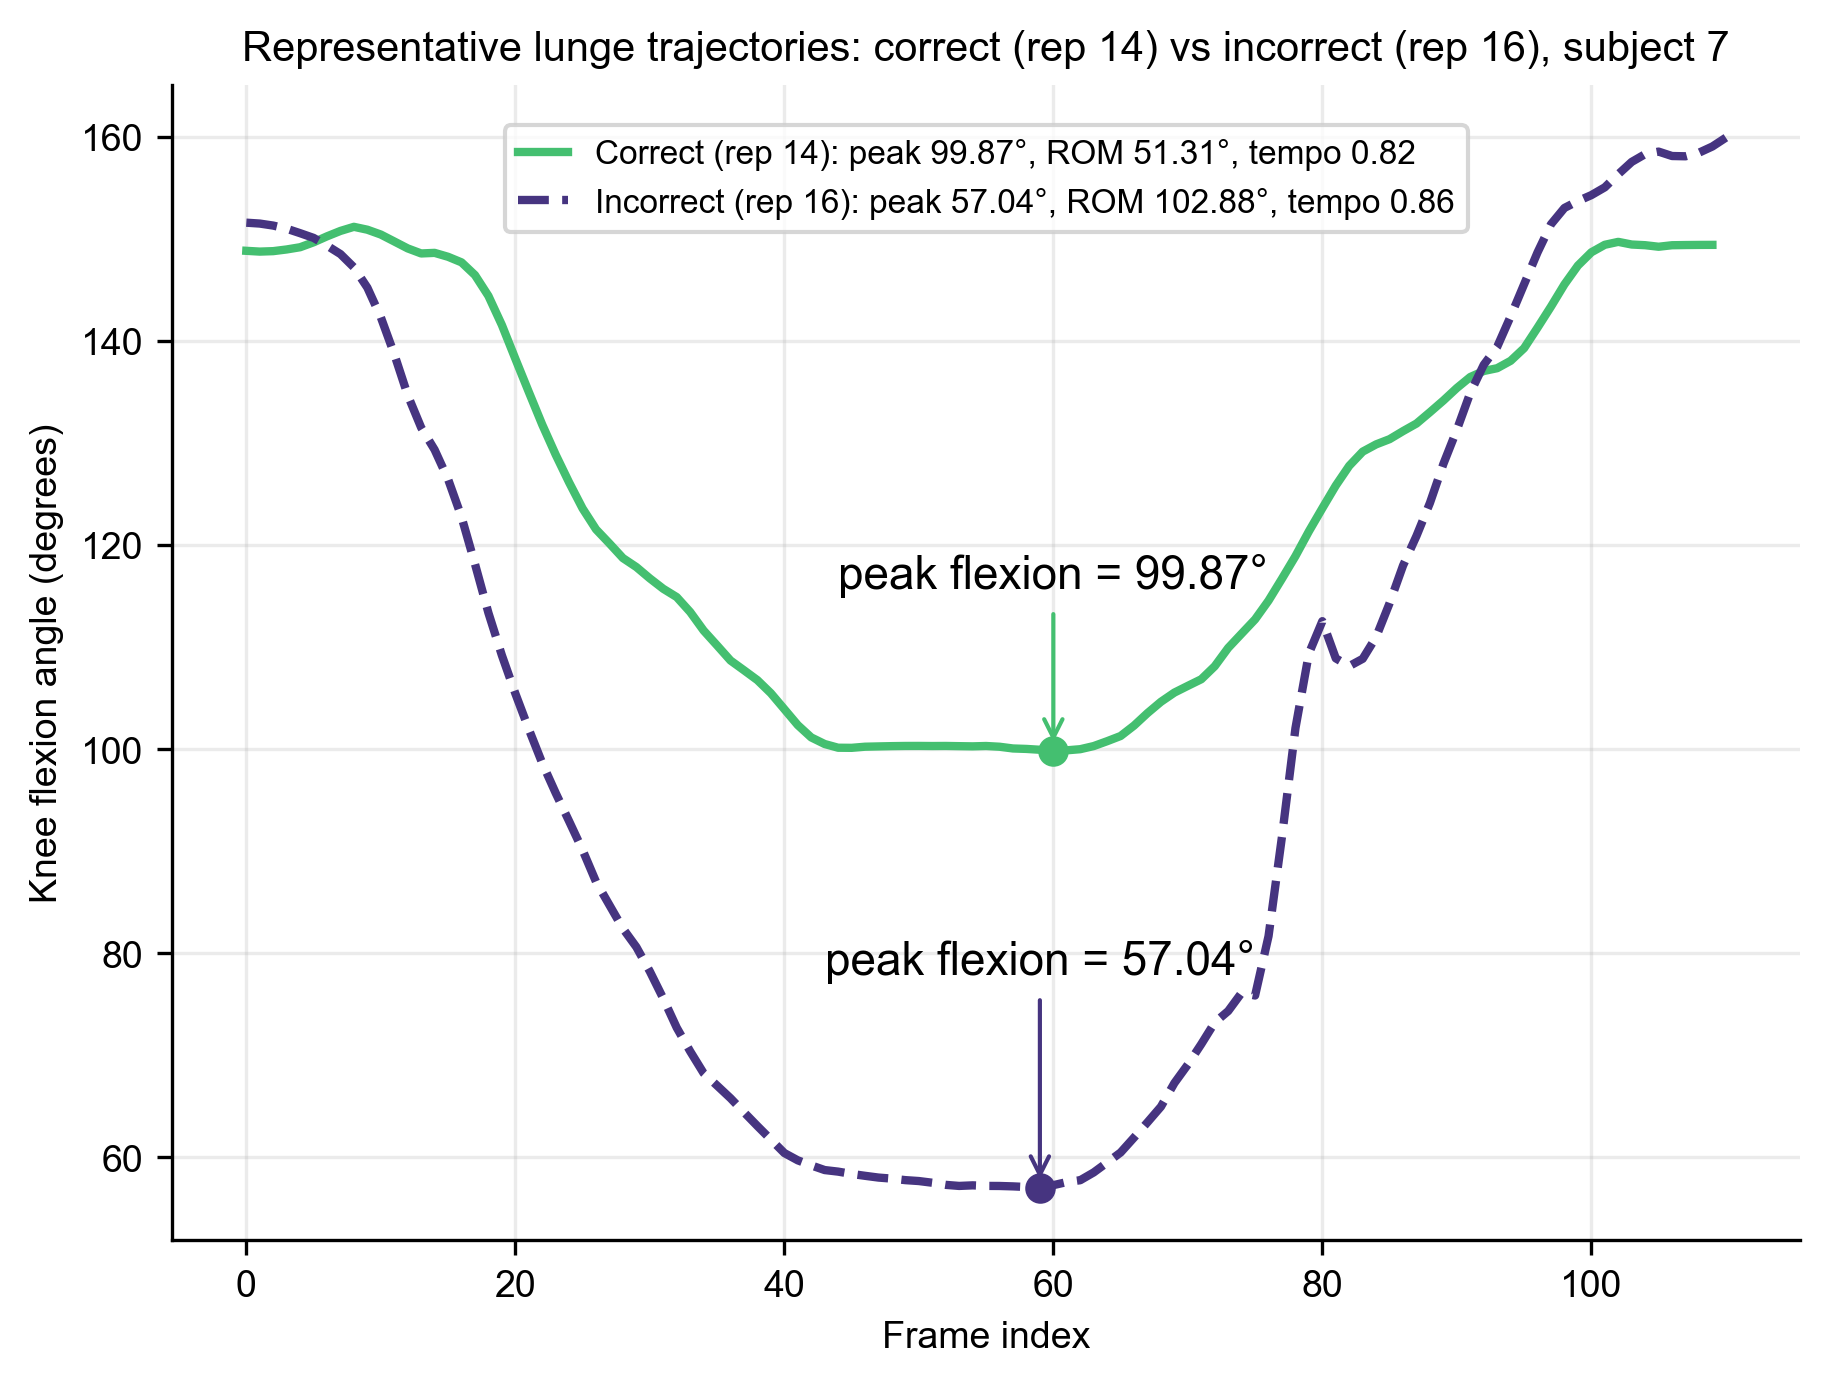
\includegraphics[width=0.92\textwidth]{fig5_4_trajectories.png}
  \caption{Representative Correct vs.\ Incorrect Knee Flexion Trajectories for Lunges. Time-series overlay illustrating descent phase and propulsive ascent velocity divergence between correct and incorrect executions.}
  \label{fig:lunge-trajectories}
\end{figure}

\chapter{Drop-Jump Validation Against Optoelectronics}
\label{ch:dropjump}

% SOURCE: results_dropjump_validation_v2.md
% STATUS: converted from markdown
% NOTE: [source:] tags stripped per ASSEMBLY_PLAN.md (harvested to appF)


This chapter presents ground-truth validation of the monocular camera pipeline (MediaPipe Heavy variant) on the OpenCap Drop-Jump dataset against synchronized 3D optoelectronic motion capture and force-plate ground truth.



\section{Temporal Synchronization and Event Detection}
\label{sec:6-1-temporal-synchronization-and-event-detection}


Joint trajectories from video and 3D motion capture were aligned across 48 trials (24 symmetric, 24 asymmetric landings across 8 subjects) using Ground Reaction Force (GRF)-anchored lag alignment.

\subsection{Synchronization Methodology}
\label{sec:6-1-1-synchronization-methodology}

The temporal anchor matched physical landing contact ($F_y > 20$ N) to kinematic flexion onset in video (local knee extension minimum). Native sample rates:
\begin{itemize}
  \item Synced video frame rate: \textbf{60.0000 FPS}.
  \item Optoelectronic Mocap IK sample rate: \textbf{100.0000 Hz}.
  \item Force plate sample rate: \textbf{2000.0000 Hz}.
\end{itemize}

\subsection{Biomarker Mapping}
\label{sec:6-1-2-biomarker-mapping}

Biomechanical events were identified via force plate and kinematic thresholds:
\begin{enumerate}
  \item \textbf{Initial Contact (IC1)}: First frame where vertical GRF exceeded $20$ N.
  \item \textbf{Peak Absorption (PA1)}: Frame containing maximum knee flexion between IC1 and takeoff (TO1).
  \item \textbf{Takeoff (TO1)}: First frame where vertical GRF dropped below $10$ N after IC1.
  \item \textbf{Final Landing Contact (IC2)}: First frame where vertical GRF exceeded $20$ N post-flight.
\end{enumerate}

These events mapped to primary knee flexion biomarkers:
\begin{itemize}
  \item \textbf{Contact Flexion (Biomarker \protect\#1)}: Knee flexion angle at \textbf{IC1}.
  \item \textbf{Peak Landing Flexion (Biomarker \protect\#2)}: Knee flexion angle at \textbf{PA1}.
  \item \textbf{Landing Range of Motion (ROM) (Biomarker \protect\#3)}: Excursion $\text{ROM} = \text{PA1} - \text{IC1}$.
  \item \textbf{Flexion Loading Rate (Biomarker \protect\#6)}: Average angular velocity during early landing ($IC1 \rightarrow \text{early absorption}$).
\end{itemize}



\section{Headline Finding: Deep-Flexion Constant Bias (Timing-Clean)}
\label{sec:6-2-headline-finding-deep-flexion-constant-bias-timing-clean}


Monocular measurement error does not scale monotonically with flexion depth across landing. Isolating static coordinate errors from dynamic synchronization lag, knee flexion was evaluated at peak absorption frames (PA1), where joint angular velocity is near zero ($\omega \approx 0$).

\subsection{Static-Peak Error Analysis}
\label{sec:6-2-1-static-peak-error-analysis}

Across $n = 96$ peak flexion points (48 trials $\times$ 2 limbs):
\begin{itemize}
  \item \textbf{Mean Deep-Flexion Bias (Video - IK)}: \textbf{$+10.52^\circ$}.
  \item \textbf{95\% Limits of Agreement (LoA)}: \textbf{$[-5.54^\circ, 26.58^\circ]$}.
\end{itemize}

\subsection{Error-vs-Depth Correlation}
\label{sec:6-2-2-error-vs-depth-correlation}

To test if overestimation is depth-dependent within active landing ($70^\circ\text{--}120^\circ$), correlations between 3D Mocap angle and error were evaluated:
\begin{itemize}
  \item Pearson correlation: $r = -0.1568$ ($p = 0.1271$).
  \item Spearman correlation: $\rho = -0.1905$ ($p = 0.0631$).
\end{itemize}

Because neither correlation was significant ($p > 0.05$), measurement error behaves as a \textbf{constant systematic positive bias} within the landing flexion band rather than a depth-dependent slope.

\subsection{Shallow Flexion Contrast}
\label{sec:6-2-3-shallow-flexion-contrast}

At initial contact (Biomarker \protect\#1, shallow flexion), the pipeline exhibits an underestimation bias of \textbf{$-6.69^\circ$}. This confirms systematic $+10.52^\circ$ overestimation is specific to deep flexion, forming a static, correctable offset.



\section{Per-Biomarker Agreement (Bland-Altman Analysis)}
\label{sec:6-3-per-biomarker-agreement-bland-altman-analysis}


Bland-Altman statistics (mean bias, 95\% LoA, Pearson $r$) across all $n = 48$ trials evaluate cohort agreement. Table 6.1 summarizes metrics across validatable biomarkers.


\begin{landscape}
\begin{table}[htbp]
\centering
\small
\caption{Bland-Altman Agreement Summary for Knee Flexion Biomarkers ($n = 48$ trials)}
\label{tab:bland-altman-summary}
\begin{tabular}{l c c c p{4.0cm} c p{4.5cm}}
\hline
\textbf{Biomarker} & \textbf{Video Mean} & \textbf{IK Mean} & \textbf{Bias (Video$-$IK)} & \textbf{95\% Limits of Agreement} & \textbf{Pearson $r$} & \textbf{Trustworthiness Verdict} \\
\hline
\textbf{\protect\#1 Contact Flexion} & $13.51^\circ$ & $20.20^\circ$ & $-6.69^\circ$ & $[-26.77^\circ,\ 13.39^\circ]$ & $0.3209$ & Accurate (low bias, moderate variance) \\
\textbf{\protect\#2 Peak Landing Flexion} & $120.23^\circ$ & $100.51^\circ$ & $+19.72^\circ$ & $[7.73^\circ,\ 31.71^\circ]$ & $0.8238$ & Biased-systematic (constant overestimation, low variance) \\
\textbf{\protect\#3 Landing ROM} & $106.72^\circ$ & $80.31^\circ$ & $+26.41^\circ$ & $[2.34^\circ,\ 50.48^\circ]$ & $0.4020$ & Biased-systematic (constant overestimation, high variance) \\
\textbf{\protect\#6 Flexion Loading Rate} & $286.14^\circ/\text{s}$ & $272.84^\circ/\text{s}$ & $+13.30^\circ/\text{s}$ & $[-115.92^\circ/\text{s},\ 142.51^\circ/\text{s}]$ & $0.6076$ & High-variance (moderate bias, high variance) \\
\textbf{\protect\#5 Asymmetry (IK-only)} & N/A & $2.07^\circ$ & N/A & N/A & N/A & \textbf{IK-only, not video-validated} (far-leg occlusion); mean$=2.07^\circ$ (SD$=2.06^\circ$) \\
\hline
\end{tabular}
\end{table}
\end{landscape}

Across biomarkers, contact flexion (\protect\#1) achieves high accuracy with minor underestimation ($-6.69^\circ$), whereas peak flexion (\protect\#2) and ROM (\protect\#3) carry systematic positive bias requiring calibration. Loading rate (\protect\#6) exhibits high variance from sampling jitter, and asymmetry (\protect\#5) is restricted to 3D IK reference data due to contralateral limb occlusion. See Appendix D for detailed biomarker-level interpretation.
Figure 6.1 presents the Bland-Altman agreement analysis for each biomarker.

\begin{figure}[htbp]
  \centering
  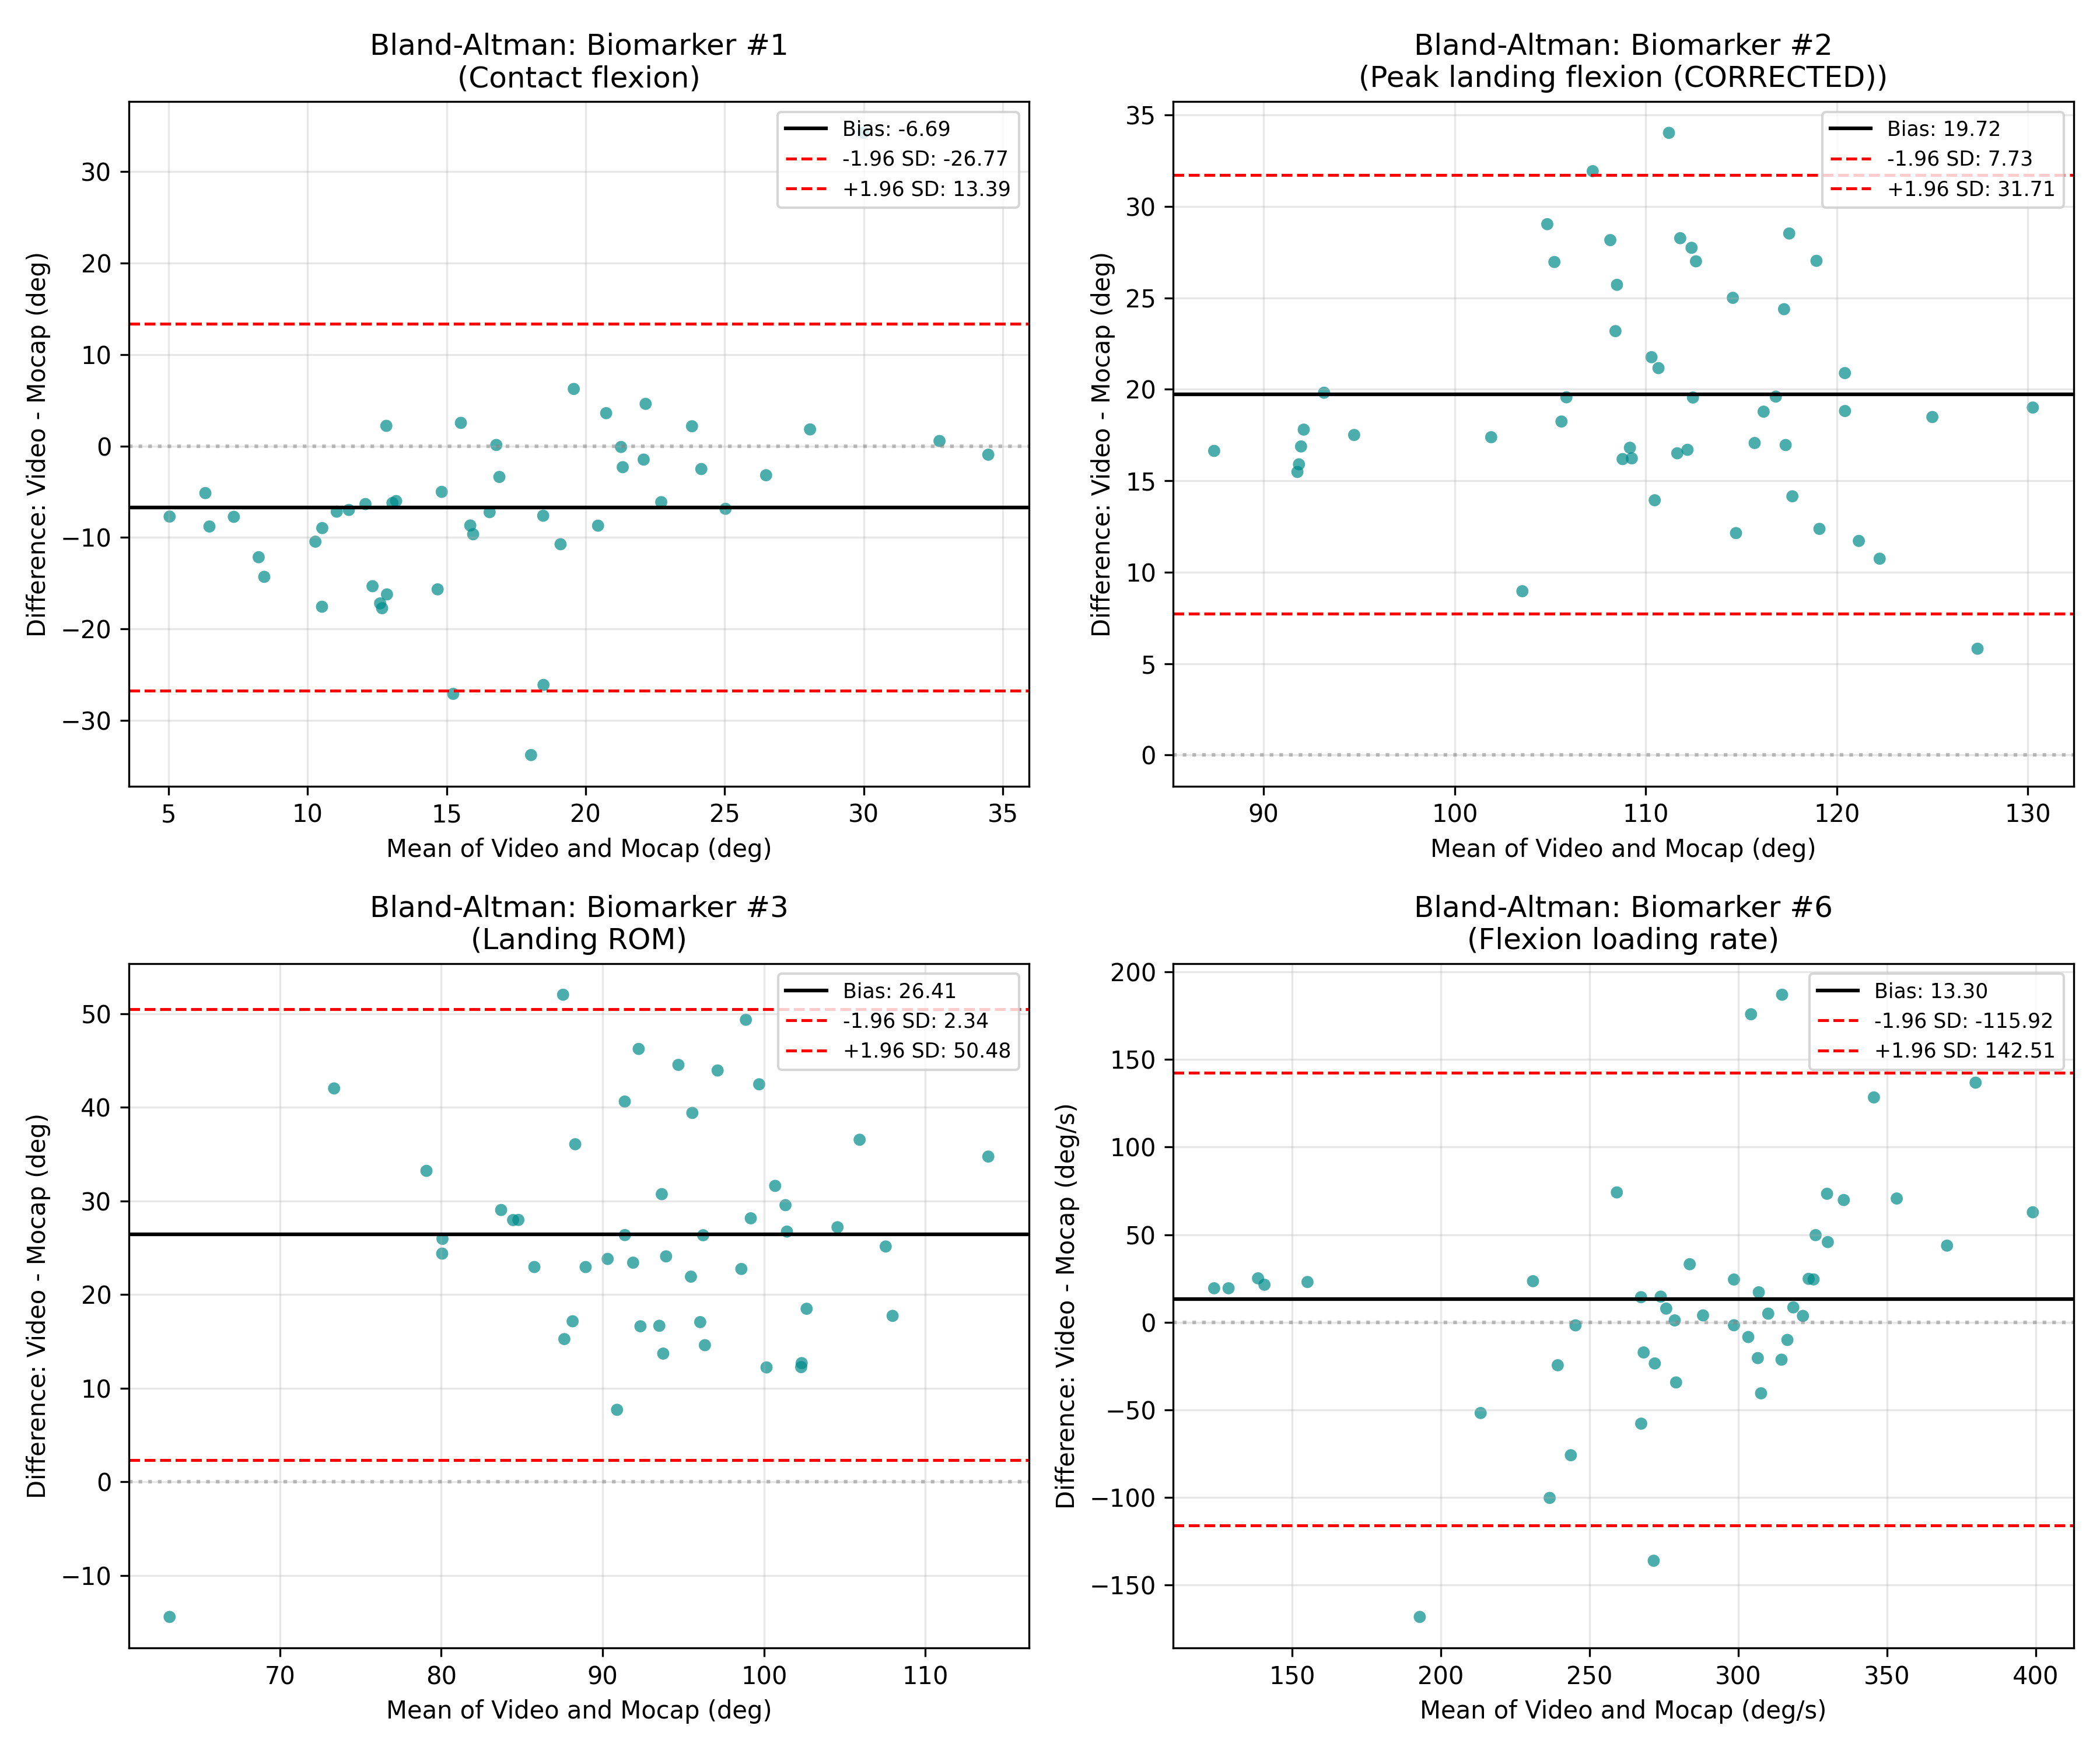
\includegraphics[width=0.95\textwidth]{fig6_1_bland_altman.png}
  \caption{Bland-Altman Agreement Plots for All Four Validatable Knee Flexion Biomarkers ($n=48$ trials). Each panel shows mean bias (solid line), 95\% Limits of Agreement (dashed), and individual trial scatter.}
  \label{fig:bland-altman-biomarkers}
\end{figure}

\begin{figure}[htbp]
  \centering
  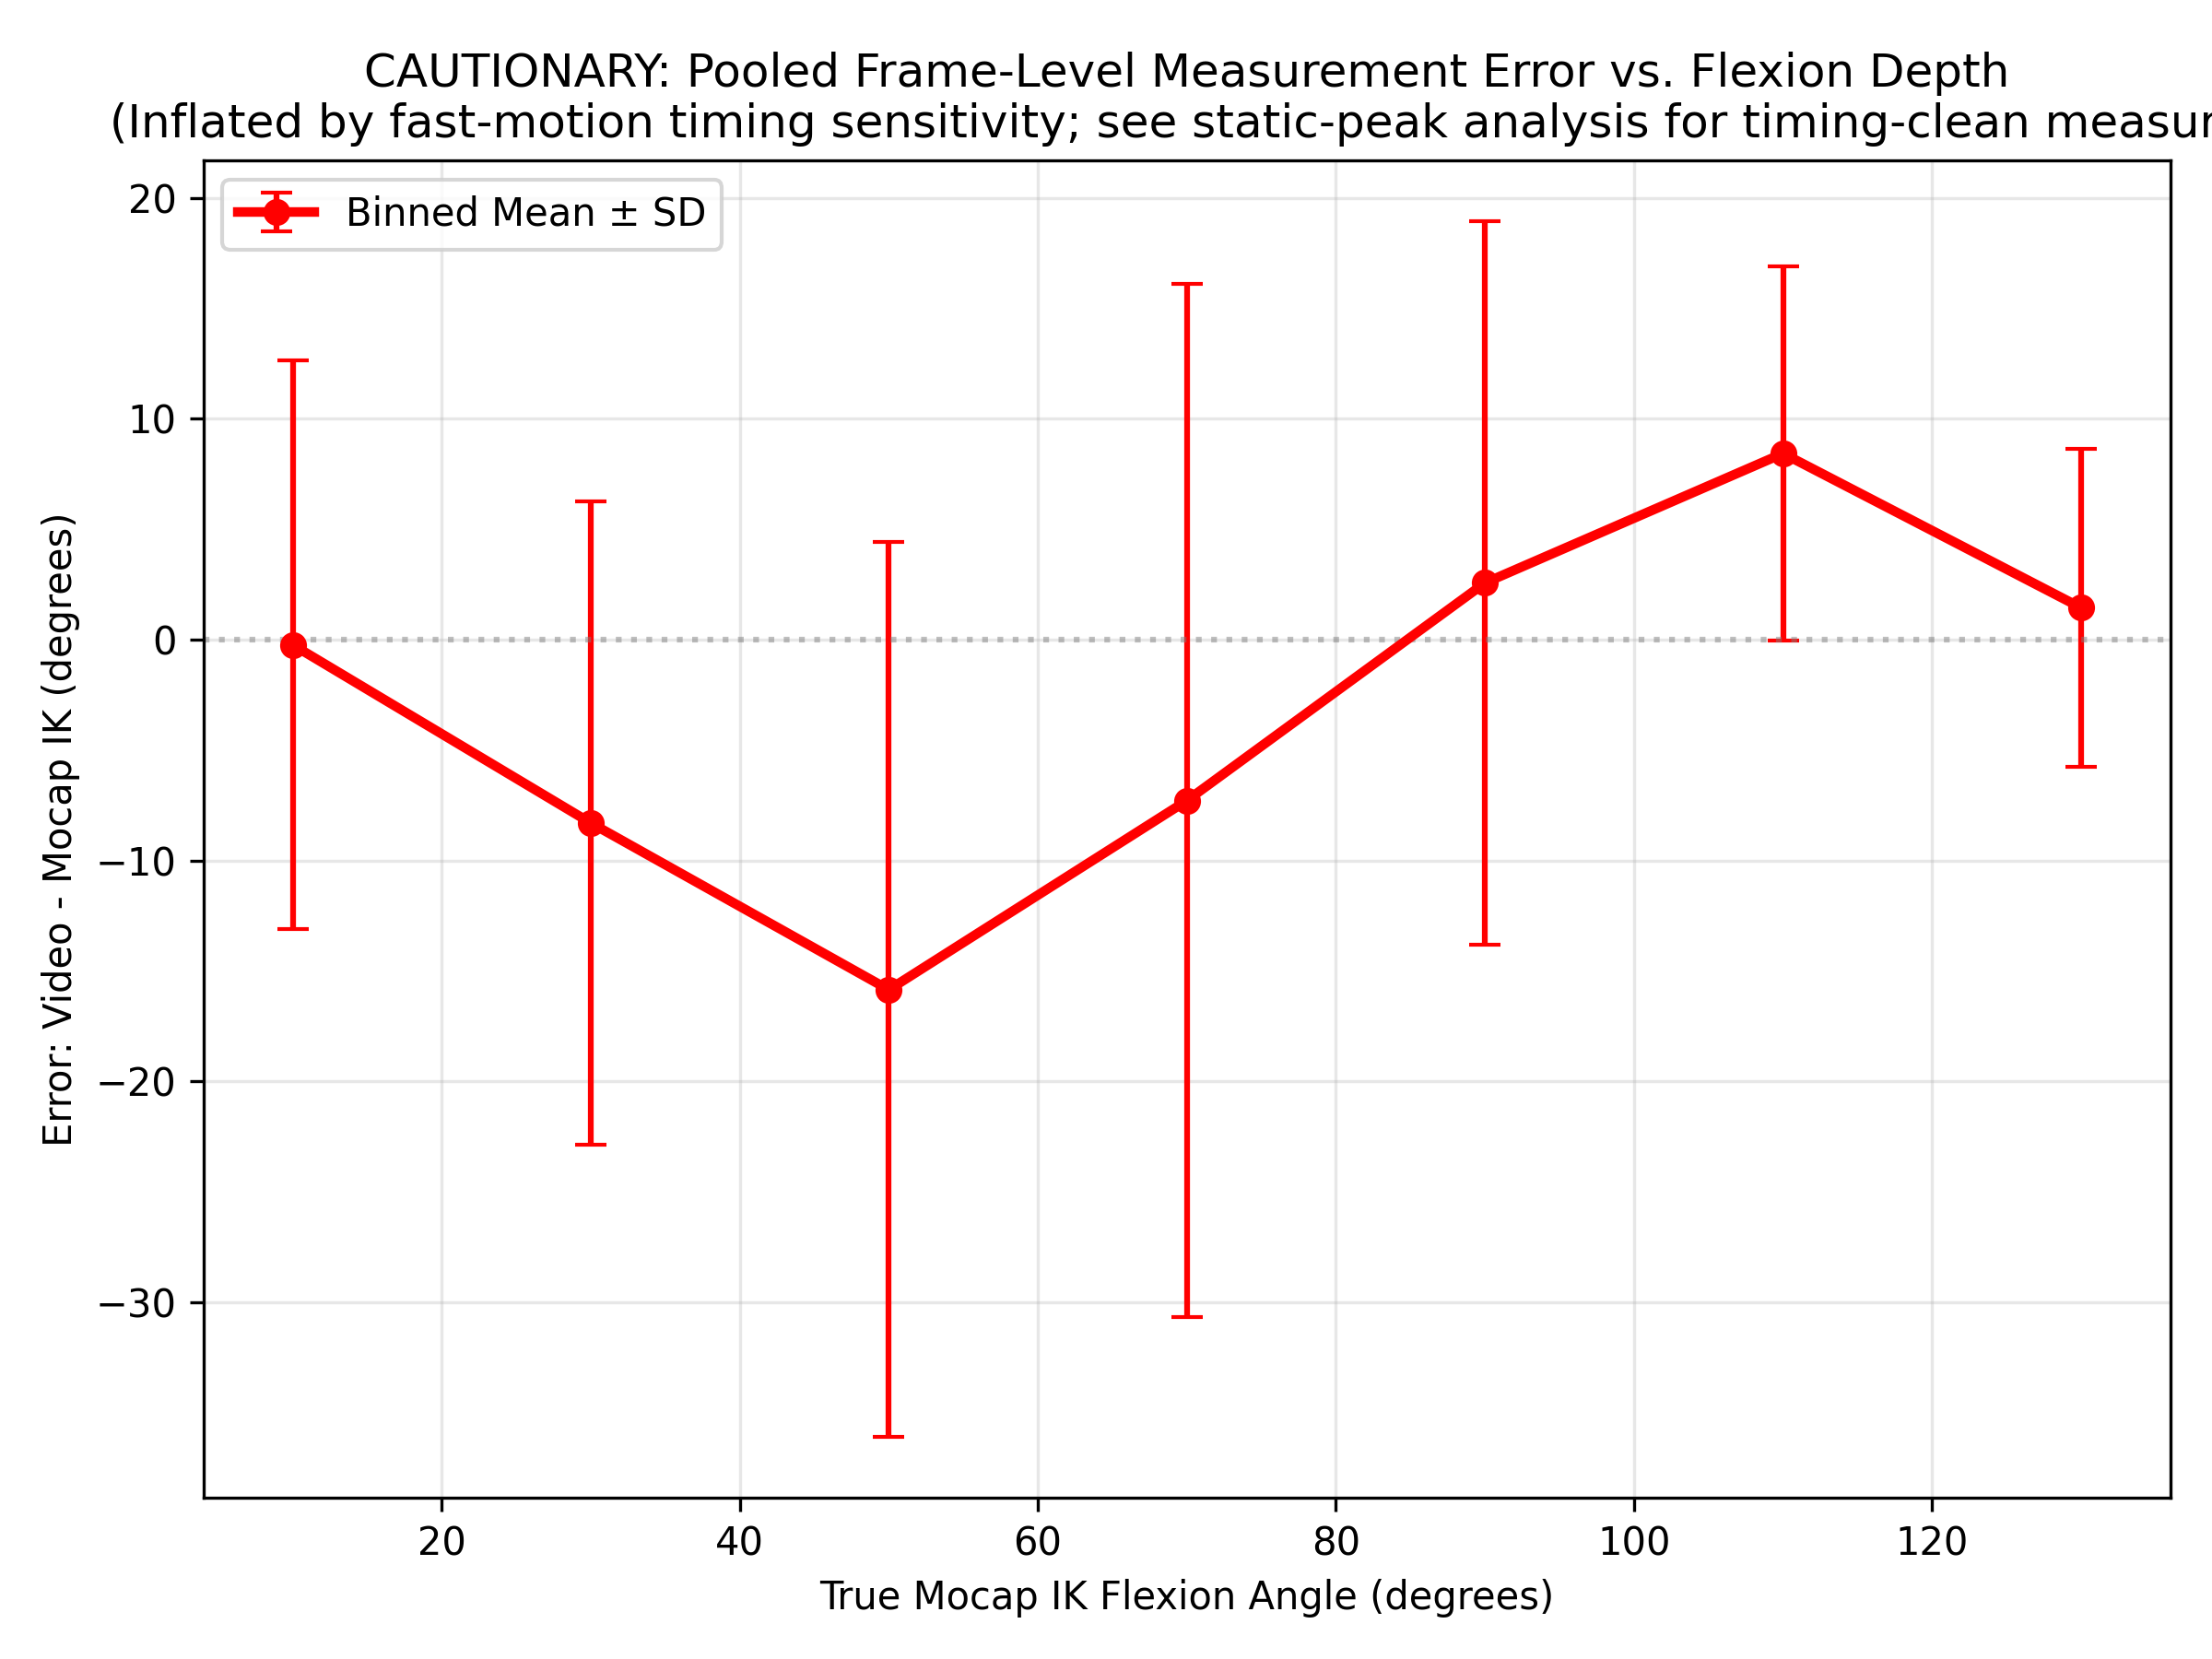
\includegraphics[width=0.82\textwidth]{fig6_2_error_vs_depth.png}
  \caption{Headline Error vs.\ Flexion Depth. Scatter plot of video--IK measurement error as a function of peak flexion depth, demonstrating depth-independent systematic bias (Pearson $r=-0.16$, $p=0.13$).}
  \label{fig:error-vs-depth}
\end{figure}

\begin{figure}[htbp]
  \centering
  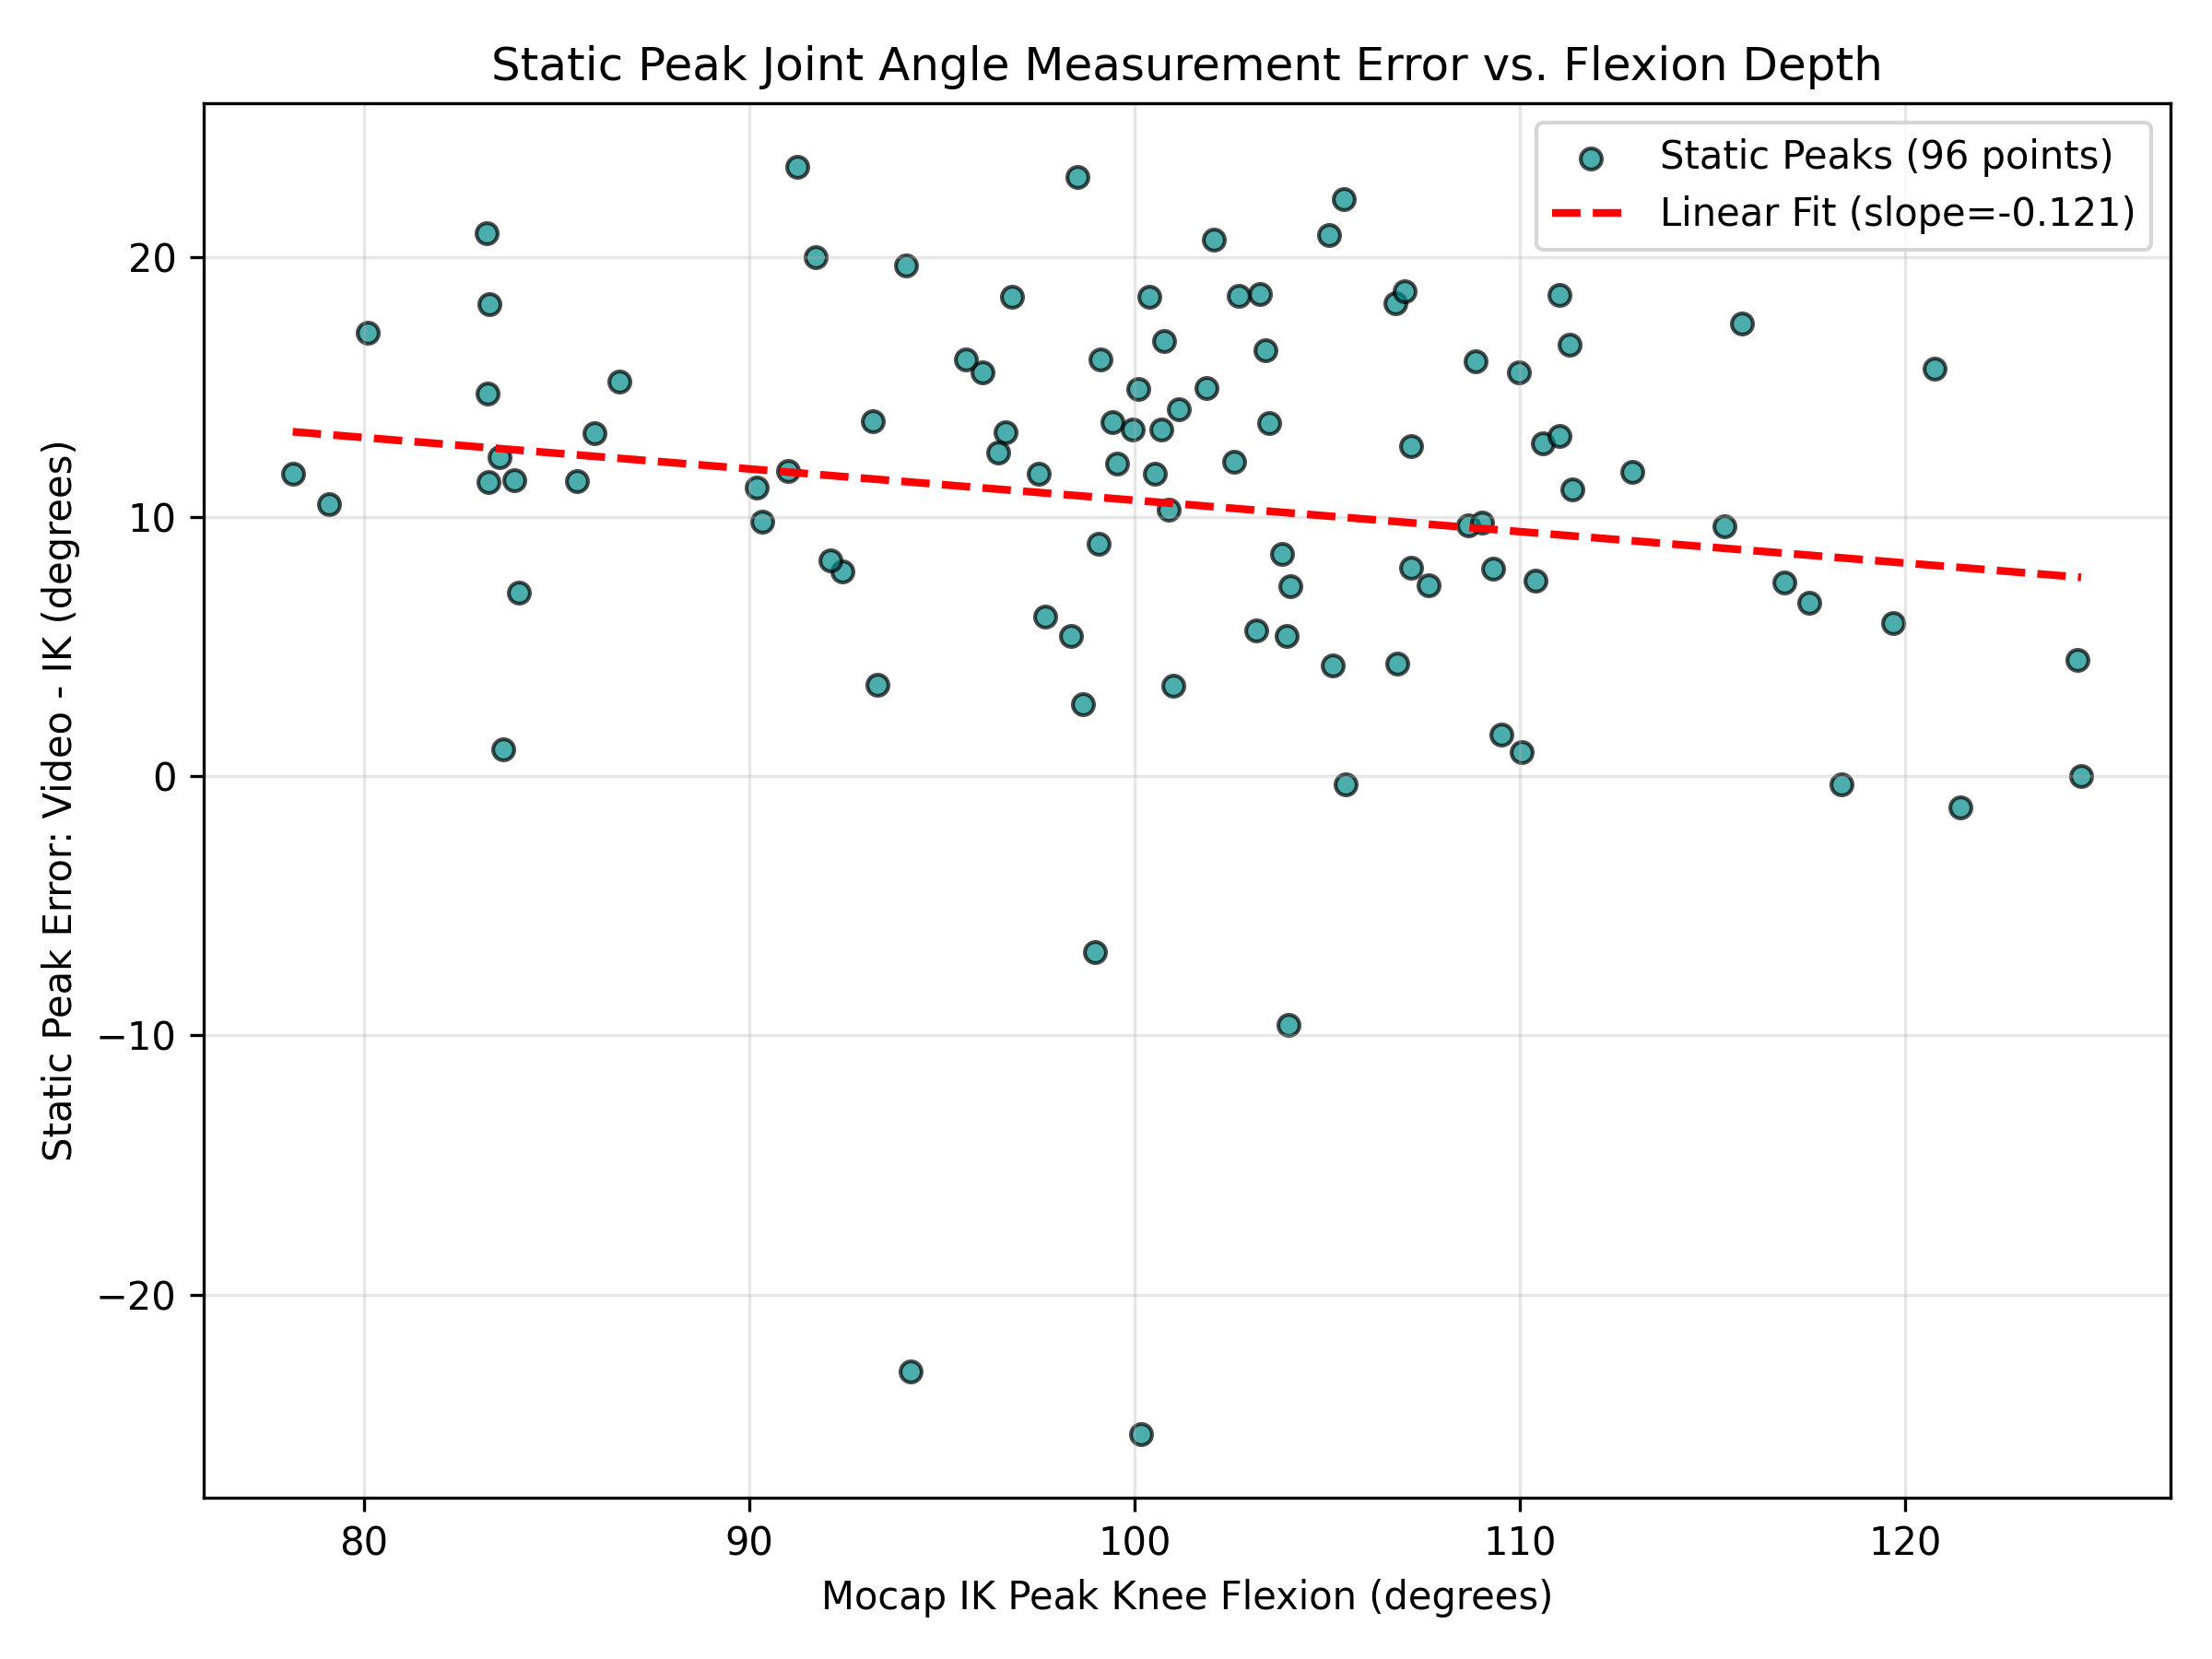
\includegraphics[width=0.72\textwidth]{fig6_3_peak_scatter.png}
  \caption{Static Peak Flexion Error Scatter. Per-trial systematic overestimation of peak flexion by monocular video relative to 3D IK, confirming the $+10.52^\circ$ timing-clean bias.}
  \label{fig:peak-scatter}
\end{figure}


\subsection{Peak-to-Peak vs. Timing-Clean Bias Reconciliation}
\label{sec:6-3-1-peak-to-peak-vs-timing-clean-bias-reconciliation}

A critical comparison emerges between the \textbf{$+10.52^\circ$ timing-clean peak bias} (Section 6.2) and the \textbf{$+19.72^\circ$ peak-to-peak bias} in Table 6.1:
\begin{itemize}
  \item \textit{Timing-Clean peak bias ($+10.52^\circ$)}: Frame-matched error at exact peak time ($t_{\text{peak}}$) of reference 3D motion capture.
  \item \textit{Peak-to-Peak bias ($+19.72^\circ$)}: Absolute maximum video trajectory value versus absolute maximum Mocap value, regardless of timing alignment.
\end{itemize}

Because 2D pose estimators experience frame-rate limits and dynamic tracking overshoot during high-velocity impact landings, unaligned peak-to-peak comparison captures temporal overshoot, inflating apparent bias by $+9.20^\circ$. For slower sagittal movements (squats, lunges) lacking impact velocities, this validation isolates the deep-flexion projection component ($\sigma^2_{\text{proj}}$), which the uncertainty-weighted framework (Chapter 8) transfers.



\section{Robustness to Movement Conditions}
\label{sec:6-4-robustness-to-movement-conditions}


To evaluate whether tracking accuracy varies with movement loading, static peak flexion errors were compared between symmetric and asymmetric landings.

\subsection{Symmetric vs. Asymmetric Landing Bias}
\label{sec:6-4-1-symmetric-vs-asymmetric-landing-bias}

\begin{itemize}
  \item \textbf{Symmetric Landings ($n = 48$ points)}: Mean peak overestimation bias \textbf{$+10.36^\circ$} (SD: $6.89^\circ$).
  \item \textbf{Asymmetric Landings ($n = 48$ points)}: Mean peak overestimation bias \textbf{$+10.68^\circ$} (SD: $9.39^\circ$).
\end{itemize}

\subsection{Methodological Implications}
\label{sec:6-4-2-methodological-implications}

The condition difference is negligible ($\Delta 0.32^\circ$). This near-identical error distribution demonstrates measurement bias is independent of kinetic landing asymmetry. Operating as a stable measurement property rather than a kinetic confound, this bias can be treated as a constant, correctable offset in downstream screening.



\section{Establishing the Bias Is Projection Error, Not Timing Artefact}
\label{sec:6-5-establishing-the-bias-is-projection-error-not-timing-artefact}


To confirm peak overestimation represents spatial projection distortion rather than temporal synchronization artefact or software modeling mismatch, three diagnostic tests were conducted.

\subsection{Dynamic Lag Test}
\label{sec:6-5-1-dynamic-lag-test}

We tested whether temporal trajectory misalignment caused deep-flexion error:
\begin{itemize}
  \item \textit{Frame-matched (GRF-aligned) MAE}: \textbf{$14.80^\circ$} (RMSE: $15.53^\circ$).
  \item \textit{Peak-matched MAE}: \textbf{$20.15^\circ$} (RMSE: $20.98^\circ$).
\end{itemize}

Forcing peak alignment worsened MAE by $5.35^\circ$ and RMSE by $5.45^\circ$. This rules out timing lag: peak-alignment forces video overshoot to match Mocap peak, increasing error and confirming spatial projection origin.

\subsection{Software Modeling Defect Test}
\label{sec:6-5-2-software-modeling-defect-test}

To rule out coordinate mismatches between clinical OpenSim models and superficial marker geometry, we compared:
\begin{enumerate}
  \item OpenSim joint coordinates from inverse kinematics output.
  \item Superficial 3-point marker trigonometric model (hip, knee, ankle) converted to clinical flexion.
\end{enumerate}

Mean offset between modeling definitions was \textbf{$1.64^\circ$} (RMSE: $21.79^\circ$ vs. $22.93^\circ$ against video), ruling out software definition mismatches as the source of $10.52^\circ$ overestimation.

\subsection{Sync Method Stability Analysis}
\label{sec:6-5-3-sync-method-stability-analysis}

Force-plate \textbf{GRF-anchored alignment} was compared against mathematical \textbf{RMSE-minimisation alignment}:
\begin{itemize}
  \item \textit{subject2 DJ1}: GRF lag = \textbf{3.00 ms (0 frames)} vs. RMSE lag = \textbf{-33.33 ms (-2 frames)}.
  \item \textit{subject2 DJAsym1}: GRF lag = \textbf{-241.17 ms (-14 frames)} vs. RMSE lag = \textbf{200.00 ms (12 frames)}.
  \item \textit{subject8 DJ1}: GRF lag = \textbf{-157.17 ms (-9 frames)} vs. RMSE lag = \textbf{33.33 ms (2 frames)}.
\end{itemize}

Because Mocap IK windows are trimmed ($\sim 1.0$ s), RMSE-minimization is unstable, choosing out-of-phase alignments (e.g., $+12$ frames, shifting video peak $0.4$ s before mocap peak). Conversely, GRF anchoring directly anchors physical impact, remaining stable across trials. Thus, GRF anchoring was adopted as standard, and pooled frame-level error-vs-depth correlation ($r = 0.3491$, $n = 3046$ frames) was demoted to a cautionary supplementary figure.
Figure 6.2 illustrates the naive pooled frame-level error plotted against knee flexion depth prior to timing diagnostic decomposition.

Diagnostics confirm deep-flexion overestimation stems from \textbf{sagittal-plane projection foreshortening}: as the knee flexes deeply outside the orthogonal camera plane, 2D projection systematically inflates apparent knee flexion angle.
Figure 6.3 demonstrates that when temporal artifacts are removed, static peak-flexion error is a constant scalar offset across flexion depths.



\section{Limitations}
\label{sec:6-6-limitations}


Limitations of dataset recording and camera configuration are documented:

\subsection{Dataset Recording Truncation (Stabilisation Time)}
\label{sec:6-6-1-dataset-recording-truncation-stabilisation-time}

Dynamic stabilisation (Biomarker \protect\#4, Time-to-Stabilisation) could not be computed. Video recordings truncate \textbf{$0.05\text{ s}$ to $0.2\text{ s}$} after final landing contact (IC2). Evaluating stabilisation requires a $0.5$ s quiet-stance window (30 frames at 60 FPS) with flexion standard deviation $< 1.5^\circ$; short recording lengths render this check unfeasible. This represents raw dataset truncation rather than pipeline failure.

\subsection{Contralateral Occlusion (Asymmetry)}
\label{sec:6-6-2-contralateral-occlusion-asymmetry}

Inter-limb asymmetry (Biomarker \protect\#5) cannot be resolved via monocular sagittal video. During deep landing absorption, the closer leg ($\sim 100\%$ tracking visibility) occludes the farther leg ($\sim 0\%$ visibility). As monocular tracking cannot resolve occluded joint landmarks, asymmetry is demoted to 3D Mocap reference data (Mocap mean: $2.07^\circ$, SD: $2.06^\circ$) and excluded from video decision rules.

\subsection{Time-Series Pooling Warnings}
\label{sec:6-6-3-time-series-pooling-warnings}

Pooled frame-level error-vs-depth displays high timing contamination and non-monotonic behavior ($r = 0.3491$). It serves as a supplementary warning against naive time-series pooling in single-camera validation.

\subsection{Kinematic Angle Conventions}
\label{sec:6-6-4-kinematic-angle-conventions}

This chapter evaluates knee flexion using \textbf{clinical flexion} ($0^\circ$ = extension, larger angle = deeper bend), contrasting with the \textbf{included angle} convention ($\approx 180^\circ$ = extension, smaller angle = deeper bend) in squat and lunge chapters. Raw angles are not directly comparable; the uncertainty-weighting framework (Chapter 8) resolves this by transferring validated error variances ($\sigma^2_{\text{proj}}$) rather than raw joint values.



\section{Figures and Provenance}
\label{sec:6-7-figures-and-provenance}


Publication-ready validation figures support this chapter:
\begin{itemize}
  \item \textbf{Figure 6.1: Bland-Altman agreement plots for peak knee flexion, contact flexion, ROM, and loading rate biomarkers}, comparing video-derived measurements against OpenCap motion-capture ground truth. The mean bias and 95\% Limits of Agreement are indicated by solid and dashed horizontal lines respectively.
  \item \textbf{Figure 6.2: Frame-level pipeline error plotted against knee flexion depth}, showing the naive pooled distribution that appears depth-dependent prior to timing diagnostic decomposition.
  \item \textbf{Figure 6.3: Static peak-flexion error plotted against ground-truth peak knee flexion depth.} The near-zero slope of the linear regression confirms that pipeline error is a constant scalar offset (approximately +10.5°) rather than a depth-dependent degradation.
\end{itemize}
\addtocounter{chapter}{1}
% Chapter 7 reserved -- deliberate gap per §1.5
\chapter{Uncertainty-Weighted Screening Framework}
\label{ch:uncertainty}

% SOURCE: results_uncertainty_framework_v2.md
% STATUS: converted from markdown
% NOTE: [source:] tags stripped per ASSEMBLY_PLAN.md (harvested to appF)


This chapter presents the design and demonstration of an uncertainty-weighted kinematic screening framework. Markerless pose-estimation pipelines capture multi-joint kinematics across several exercises, but measurement accuracy across joint angle biomarkers is unequal. To address this, we present an architectural framework that weights each screening biomarker inversely proportional to its ground-truth-validated measurement uncertainty. First, we outline the purpose and design motivation. Second, we convert the drop-jump limits of agreement (LoA) validated in Chapter 6 into statistical variances. Third, we present the projection/motion error decomposition that isolates geometry-general perspective errors from drop-jump-specific timing sensitivity. Fourth, we apply inverse-variance weighting to establish cross-exercise transfer weights. Finally, we demonstrate the framework's behavior through worked examples in squats and lunges. The full mathematical derivation is provided in Appendix A.



\section{Purpose and Design Motivation}
\label{sec:8-1-purpose-and-design-motivation}


Monocular, single-camera biomechanical screening offers significant scalability over marker-based laboratory systems. However, single-camera tracking is subject to several error components—including perspective foreshortening, self-occlusion, sub-frame synchronization mismatch, and motion blur. In Chapter 6, we conducted a ground-truth validation pass comparing monocular video-derived drop-jump biomarkers against 3D optical motion capture, establishing the 95\% Limits of Agreement (LoA) for each metric.

The primary motivation of this chapter is converting those validated measurement error bounds into a per-biomarker weighting scheme that qualifies how much to trust each joint angle metric during multi-exercise screening. Rather than treating all extracted joint angles with equal confidence, the screening framework propagates these validated uncertainties to the squat and lunge evaluations discussed in Chapters 4 and 5.

\subsection{Hard Architectural Constraints and Scope}
\label{sec:8-1-1-hard-architectural-constraints-and-scope}

To prevent misinterpretation, we establish strict scope boundaries for this framework:
\begin{enumerate}
  \item \textbf{No Risk Scoring}: The framework does not calculate a risk index or predict clinical outcomes. It is strictly an architectural characterisation of measurement uncertainty.
  \item \textbf{No Repetition Classification}: It does not classify individual repetitions or label movement as "good" or "bad".
  \item \textbf{Architectural Demonstration Only}: It is a design demonstration showing how validated measurement uncertainties propagate across exercises, not a deployed clinical software system.
\end{enumerate}



\section{Uncertainty Source and Variance Conversion}
\label{sec:8-2-uncertainty-source-and-variance-conversion}


The source of truth for measurement uncertainty is the drop-jump cohort validation agreement table (\texttt{phase6\_agreement\_final.csv}), validating $n = 48$ drop-jump trials across $8$ subjects.

\subsection{Converted Biomarker Variances}
\label{sec:8-2-1-converted-biomarker-variances}

Assuming normally distributed errors ($3.92 \text{ SD} = \text{LoA}_{\text{upper}} - \text{LoA}_{\text{lower}}$), validated drop-jump LoA bounds convert into the following statistical variances ($\sigma^2_{\text{total}}$):

\begin{enumerate}
  \item \textbf{\protect\#1 contact\_flexion}: 95\% LoA $[-26.7742^\circ, 13.3913^\circ]$ (Width: $40.1655^\circ$, Bias: $-6.6914^\circ$) $\implies \text{SD} = 10.2463^\circ$, $\sigma^2_{\text{total}} = \mathbf{104.9867}$.
  \item \textbf{\protect\#2 peak\_landing\_flexion}: 95\% LoA $[7.7285^\circ, 31.7057^\circ]$ (Width: $23.9772^\circ$, Bias: $+19.7171^\circ$) $\implies \text{SD} = 6.1166^\circ$, $\sigma^2_{\text{total}} = \mathbf{37.4132}$.
  \item \textbf{\protect\#3 landing\_rom}: 95\% LoA $[2.3373^\circ, 50.4798^\circ]$ (Width: $48.1425^\circ$, Bias: $+26.4086^\circ$) $\implies \text{SD} = 12.2813^\circ$, $\sigma^2_{\text{total}} = \mathbf{150.8291}$.
  \item \textbf{\protect\#6 loading\_rate}: 95\% LoA $[-115.9179^\circ/\text{s}, 142.5125^\circ/\text{s}]$ (Width: $258.4304^\circ/\text{s}$, Bias: $+13.2973^\circ/\text{s}$) $\implies \text{SD} = 65.9261^\circ/\text{s}$, $\sigma^2_{\text{total}} = \mathbf{4346.2534}$.
\end{enumerate}

\subsection{Exclusion of Asymmetry}
\label{sec:8-2-2-exclusion-of-asymmetry}

Biomarker \protect\#5 (landing asymmetry) is a 3D-only reference metric. Monocular sagittal video suffers complete contralateral occlusion of the far leg during deep landing absorption, precluding ground-truth validation against motion capture. It is therefore excluded from the video uncertainty framework.



\section{Projection/Motion Error Decomposition}
\label{sec:8-3-projection-motion-error-decomposition}


To transfer validated drop-jump uncertainty bounds to other sagittal movements, we decompose total measurement variance ($\sigma^2_{\text{total}}$) into two underlying components:
\begin{equation}
  \sigma^2_{\text{total}} = \sigma^2_{\text{proj}} + \sigma^2_{\text{mot}}
  \label{eq:disp1}
\end{equation}

\subsection{Rationale for Variance Splitting}
\label{sec:8-3-1-rationale-for-variance-splitting}

The physical rationale for splitting variance rests on measurement geometry:
\begin{enumerate}
  \item \textbf{Projection Error ($\sigma^2_{\text{proj}}$)}: Systematic geometric distortion caused by 2D camera sensor projection of out-of-plane joint rotation. Dictated by perspective foreshortening, this component is general to monocular sagittal pose estimation and transfers to any sagittal movement where the knee flexes in plane (such as squats and lunges).
  \item \textbf{Motion Error ($\sigma^2_{\text{mot}}$)}: Dynamic timing-sensitivity error caused by sub-frame synchronization lag and motion blur. This component is specific to the rapid-landing impact window of drop-jumps and does not transfer to slow, controlled movements like squats and lunges.
\end{enumerate}

\subsection{Decomposed Biomarker Components}
\label{sec:8-3-2-decomposed-biomarker-components}

Decomposing each biomarker based on landing biomechanics yields:
\begin{itemize}
  \item \textbf{Peak Landing Flexion (\protect\#2)}: Measured at peak absorption where knee angular velocity is near zero ($\omega \approx 0$). Static peak error is purely spatial: $\sigma^2_{\text{proj}} = \mathbf{37.4132}$ ($100.0\%$), $\sigma^2_{\text{mot}} = \mathbf{0.0000}$ ($0.0\%$).
  \item \textbf{Contact Flexion (\protect\#1)}: Measured at landing contact near full extension. Assuming a $90/10$ split yields $\sigma^2_{\text{proj}} = \mathbf{94.4880}$ ($90.0\%$), $\sigma^2_{\text{mot}} = \mathbf{10.4987}$ ($10.0\%$).
  \item \textbf{Flexion Loading Rate (\protect\#6)}: Rapid impact velocity metric dominated by sub-frame contact timing. Assuming a $10/90$ split yields $\sigma^2_{\text{proj}} = \mathbf{434.6253}$ ($10.0\%$), $\sigma^2_{\text{mot}} = \mathbf{3911.6281}$ ($90.0\%$).
  \item \textbf{Landing ROM (\protect\#3)}: Propagated from peak (\protect\#2) and contact (\protect\#1) endpoints ($\sigma^2_{\text{proj, ROM}} = 37.4132 + 94.4880 = 131.9012$). Scaled to observed total ($150.8291$), this gives a $92.62\% / 7.38\%$ split: $\sigma^2_{\text{proj}} = \mathbf{139.7047}$, $\sigma^2_{\text{mot}} = \mathbf{11.1244}$.
\end{itemize}

Sensitivity analysis confirmed weight ordering stable across assumed projection/motion splits, with weights varying less than 8.6\%; full sweep details are in Appendix A.



\section{Cross-Exercise Weight Transfer and Inverse-Variance Weighting}
\label{sec:8-4-cross-exercise-weight-transfer-and-inverse-variance-weighting}


To aggregate measurements of unequal precision, we apply standard \textbf{inverse-variance weighting} \citep{Borenstein_2013}, where each raw weight is $w_i = 1 / \sigma_i^2$ and normalized weight is $\bar{w}_i = w_i / \sum w_j$.

\subsection{Transfer Rule and Biomarker Mapping}
\label{sec:8-4-1-transfer-rule-and-biomarker-mapping}

Slow, controlled movements—such as squats and lunges—occur at low joint angular velocities where dynamic timing jitter ($\sigma^2_{\text{mot}}$) is biomechanically negligible. When transferring uncertainty weights to squats and lunges, we discard non-transferable motion variance and use \textbf{only the transferable projection component} ($\sigma^2_{\text{proj}}$):
\begin{equation}
  w_{\text{proj}, i} = \frac{1}{\sigma^2_{\text{proj}, i}}
  \label{eq:disp2}
\end{equation}

This transfer maps drop-jump biomarkers to squat/lunge equivalents based on shared sagittal biomechanics:
\begin{itemize}
  \item \texttt{contact\_flexion} $\leftrightarrow$ \texttt{start\_flexion}: Both capture shallow flexion near full extension ($180^\circ$) where perspective error is minimal.
  \item \texttt{loading\_rate} $\leftrightarrow$ \texttt{descent\_velocity}: Both capture angular flexion velocity ($\circ/\text{s}$).
\end{itemize}

\subsection{Transferable Squat and Lunge Weights}
\label{sec:8-4-2-transferable-squat-and-lunge-weights}

Computing inverse-variance weights from projection variances ($\sigma^2_{\text{proj}}$) yields normalized cross-exercise transfer weights:
\begin{enumerate}
  \item \textbf{Peak Flexion}: \textbf{$57.15\%$} (Dominates screening characterisation due to low projection variance)
  \item \textbf{Start Flexion}: \textbf{$22.63\%$}
  \item \textbf{Range of Motion (ROM)}: \textbf{$15.30\%$}
  \item \textbf{Joint Descent Velocity}: \textbf{$4.92\%$} (Down-weighted due to higher projection uncertainty)
\end{enumerate}



\section{Worked Example Demonstration}
\label{sec:8-5-worked-example-demonstration}


The framework was demonstrated using representative correct and incorrect reps from the REHAB24-6 dataset:
\begin{itemize}
  \item \textbf{Squat Reps}: Subject \texttt{PM\_008} (Subject 1) rep 2 (correct) and rep 17 (incorrect).
  \item \textbf{Lunge Reps}: Subject \texttt{PM\_021} (Subject 2) rep 2 (correct) and rep 7 (incorrect).
\end{itemize}

\subsection{Validated Noise Floors}
\label{sec:8-5-1-validated-noise-floors}

For each biomarker, $95\%$ measurement confidence half-widths (noise floors) around raw video values are calculated using transferable projection standard deviations ():
\begin{equation}
  \text{SD}_{\text{proj}} = \sqrt{\sigma^2_{\text{proj}}}
  \label{eq:auto3}
\end{equation}
\begin{itemize}
  \item \textbf{\texttt{start\_flexion} floor}:
\begin{equation}
  1.96 \times \sqrt{94.4880} = \mathbf{\pm 19.05^\circ}
  \label{eq:auto4}
\end{equation}
  \item \textbf{\texttt{peak\_flexion} floor}:
\begin{equation}
  1.96 \times \sqrt{37.4132} = \mathbf{\pm 11.99^\circ}
  \label{eq:auto5}
\end{equation}
  \item \textbf{\texttt{rom} floor}:
\begin{equation}
  1.96 \times \sqrt{139.7047} = \mathbf{\pm 23.17^\circ}
  \label{eq:auto6}
\end{equation}
  \item \textbf{\texttt{velocity} floor}:
\begin{equation}
  1.96 \times \sqrt{434.6253} = \mathbf{\pm 40.86^\circ/\text{s}}
  \label{eq:auto7}
\end{equation}
\end{itemize}

These bounds represent the markerless system's validated physical measurement precision, remaining constant across repetitions by construction.

\subsection{Worked Example Data}
\label{sec:8-5-2-worked-example-data}

Table 8.1 presents raw video measurements alongside validated uncertainty bounds and normalized weights:


\begin{table}[htbp]
\centering
\scriptsize
\setlength{\tabcolsep}{3pt}
\renewcommand{\arraystretch}{1.2}
\caption{Worked Example Repetitions for Squat and Lunge Modalities}
\label{tab:table-8-1-worked-example-repetitions-for-squat-and-lunge-modalities}
\begin{tabular}{@{}p{1.3cm} >{\centering\arraybackslash}p{1.4cm} >{\centering\arraybackslash}p{0.8cm} >{\centering\arraybackslash}p{1.4cm} >{\centering\arraybackslash}p{2.2cm} >{\centering\arraybackslash}p{2.2cm} >{\centering\arraybackslash}p{2.2cm} >{\centering\arraybackslash}p{2.3cm}@{}}
\hline
\textbf{Exercise} & \textbf{Video ID} & \textbf{Rep} & \textbf{Form} & \textbf{Start Flexion} ($^\circ$) & \textbf{Peak Flexion} ($^\circ$) & \textbf{ROM} ($^\circ$) & \textbf{Velocity} ($^\circ$/s) \\
\hline
Squat & \texttt{PM\_008} & 2 & Correct & $0.82^\circ \pm 19.05^\circ$ & $62.16^\circ \pm 11.99^\circ$ & $117.02^\circ \pm 23.17^\circ$ & $58.51^\circ/\text{s} \pm 40.86^\circ/\text{s}$ \\
Squat & \texttt{PM\_008} & 17 & Incorrect & $2.23^\circ \pm 19.05^\circ$ & $50.03^\circ \pm 11.99^\circ$ & $127.73^\circ \pm 23.17^\circ$ & $105.18^\circ/\text{s} \pm 40.86^\circ/\text{s}$ \\
Lunge & \texttt{PM\_021} & 2 & Correct & $21.42^\circ \pm 19.05^\circ$ & $83.53^\circ \pm 11.99^\circ$ & $75.05^\circ \pm 23.17^\circ$ & $27.12^\circ/\text{s} \pm 40.86^\circ/\text{s}$ \\
Lunge & \texttt{PM\_021} & 7 & Incorrect & $18.51^\circ \pm 19.05^\circ$ & $54.65^\circ \pm 11.99^\circ$ & $106.84^\circ \pm 23.17^\circ$ & $69.57^\circ/\text{s} \pm 40.86^\circ/\text{s}$ \\
\hline
\end{tabular}
\end{table}

This demonstration highlights how the framework down-weights joint velocity ($4.92\%$) relative to peak flexion depth ($57.15\%$). Peak depth deviations are characterized with high confidence (narrower CI of $\pm 11.99^\circ$), whereas velocity deviations carry wider relative uncertainty ($\pm 40.86^\circ/\text{s}$).
Figure 8.1 illustrates the worked example of the uncertainty-weighted biomarker framework across the four biomarkers.

\begin{figure}[htbp]
  \centering
  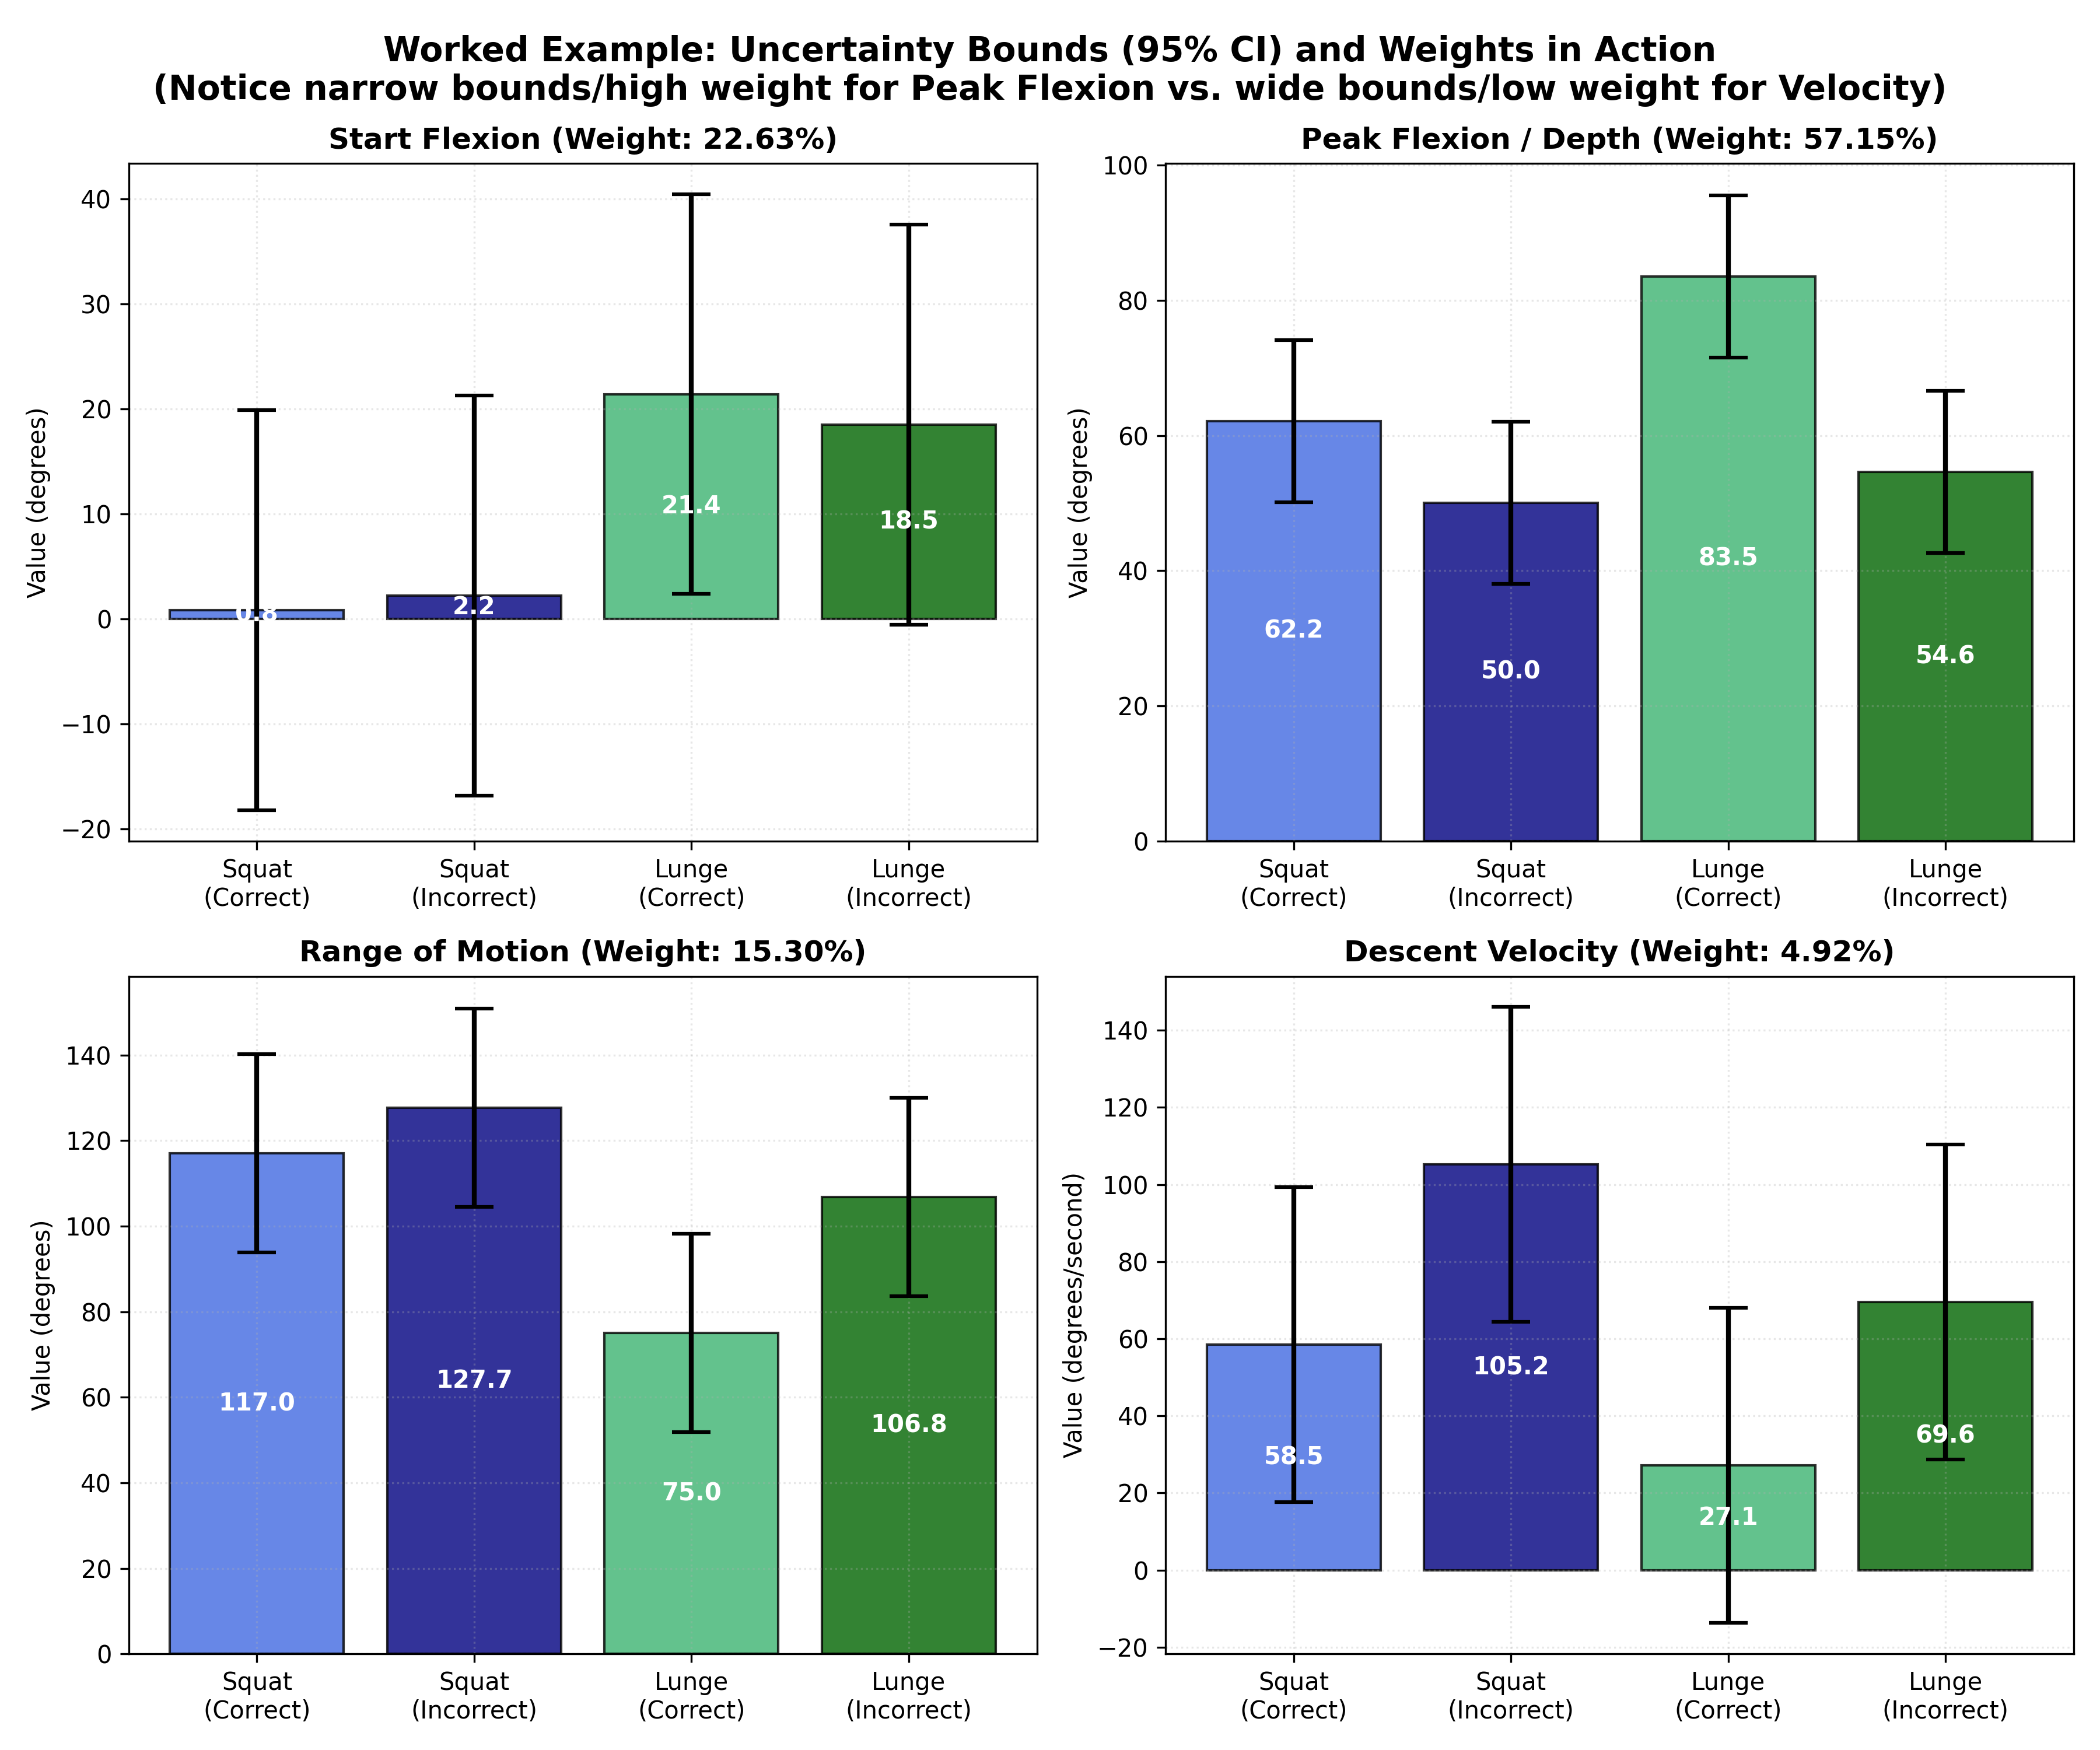
\includegraphics[width=0.88\textwidth]{fig8_1_weights.png}
  \caption{Worked Example: Uncertainty-Weighted Biomarker Framework. Each biomarker's validated 95\% confidence bounds and derived inverse-variance weight are shown. Peak flexion has the tightest bounds ($\pm 11.99^\circ$) and receives the largest weight (57.15\%); descent velocity has the widest bounds ($\pm 40.86^\circ/\text{s}$) and receives the smallest weight (4.92\%).}
  \label{fig:uncertainty-weights}
\end{figure}




\section{Empirical Confirmation Across Dissertation Components}
\label{sec:8-6-empirical-confirmation-across-dissertation-components}


The theoretical prediction of peak flexion dominance ($57.15\%$ weight) is independently confirmed by two subsequent empirical chapters:
\begin{enumerate}
  \item \textbf{Personalised Longitudinal Baselines (Chapter 9)}: Repetition-level screening gating demonstrated that screening triggers are overwhelmingly driven by peak flexion deviations beyond the tight $\pm 11.99^\circ$ noise floor, while velocity remains quiet due to its broad $\pm 40.86^\circ/\text{s}$ floor.
  \item \textbf{Temporal Sequence Models (Chapter 13)}: Leave-One-Subject-Out (LOSO) cross-validation established that peak flexion alone achieves optimal classification performance ($81.36\%$ squat / $81.50\%$ lunge balanced accuracy), outperforming complex trajectory shape models.
\end{enumerate}



\section{What This Framework Does NOT Claim}
\label{sec:8-7-what-this-framework-does-not-claim}


To maintain scientific integrity, we define explicit boundaries for the framework:
\begin{itemize}
  \item \textbf{No Diagnostic Claims}: Does not predict ACL injury, patellofemoral pain, or pathology.
  \item \textbf{No Injury Risk Scoring}: Does not synthesize weighted biomarkers into a risk score or hazard ratio.
  \item \textbf{No Repetition Classification}: Does not label repetitions as "passed" or "failed".
  \item \textbf{No Validation of Squat/Lunge Motion Error}: Motion error validation for slow exercises remains future work.
  \item \textbf{Methodological Demonstration Only}: Worked examples illustrate uncertainty propagation rather than a clinical diagnostic tool.
\end{itemize}



\section{Figures and Provenance}
\label{sec:8-8-figures-and-provenance}


Publication-ready framework figures support this chapter:
\begin{itemize}
  \item \textbf{Figure 8.1: Worked example of the uncertainty-weighted biomarker framework}, showing each biomarker's validated 95\% confidence bounds and derived inverse-variance weight. Peak flexion has the tightest bounds (±11.99°) and receives the largest weight (57.15\%); descent velocity has the widest bounds (±40.86°/s) and receives the smallest weight (4.92\%).
\end{itemize}
\chapter{Personalised Session-to-Session Baselines}
\label{ch:baseline}

% SOURCE: results_baseline_v2.md
% STATUS: converted from markdown
% NOTE: [source:] tags stripped per ASSEMBLY_PLAN.md (harvested to appF)


This chapter presents the design and empirical demonstration of an individualised kinematic progression-tracking framework. Group-level cohort analyses (Chapters 4 and 5) evaluate differences across populations, but clinical rehabilitation and performance tracking require monitoring an individual relative to their own baseline template. We describe an architecture that constructs a personalised baseline from a subject's initial correct repetitions and gates subsequent trials against the monocular pipeline's validated measurement-noise floor derived in Chapter 8.



\section{Purpose and Design Motivation}
\label{sec:9-1-purpose-and-design-motivation}


Group-level cohort analyses demonstrate population-wide execution differences. However, clinical therapy and athletic coaching are fundamentally individualised. Every athlete possesses unique anatomical constraints, prior injury histories, and movement habits that shift their baseline joint kinematics. Consequently, group-averaged templates are poor references for longitudinal tracking, as an individual's normal movement variation may fall outside cohort means without indicating movement pathology.

This framework shifts the unit of analysis from the cohort to the individual. By building a baseline from early correct trials, the framework monitors subsequent performance relative to the individual's "normal" template. Crucially, a shift is flagged as a real kinematic change only if it exceeds the monocular camera's validated measurement-noise floor (derived in Chapter 8), preventing false alarms from normal execution variability or camera perspective offsets.

\subsection{Pseudo-Timepoint Axis and Scope}
\label{sec:9-1-1-pseudo-timepoint-axis-and-scope}

Because public physical therapy datasets (including REHAB24-6) are collected during a single laboratory session, we employ \textbf{within-session repetition order} as a \textbf{pseudo-time axis}: the first repetitions represent the baseline reference period, while subsequent repetitions represent observation points over pseudo-time. This pseudo-time axis demonstrates the gating architecture; the methodology generalizes directly to multi-session longitudinal tracking across days or weeks (future work).



\section{Baseline Construction and Gating Rules}
\label{sec:9-2-baseline-construction-and-gating-rules}


The framework operates in two sequential stages: baseline building and test sequence gating.

\subsection{Personalized Baseline Building}
\label{sec:9-2-1-personalized-baseline-building}

The baseline is constructed from a subject's first \textbf{2 correct repetitions} (Reps 1 and 2). Selecting early correct repetitions establishes a clean reference template prior to the onset of movement fatigue or instructed form deviations:
\begin{itemize}
  \item \textbf{Baseline Mean Reference ($\mu_{\text{base}, i}$)}: Mean of biomarker $i$ computed across baseline repetitions:
\begin{equation}
  \mu_{\text{base}, i} = \frac{1}{2} (x_{1, i} + x_{2, i})
  \label{eq:disp1}
\end{equation}
  \item \textbf{Baseline Standard Deviation ($SD_{\text{base}, i}$) [Descriptive Only]}: Reported solely as descriptive context for early-session consistency (). It is \textbf{not} used in gating because $n = 2$ is statistically unstable and would induce false flags.
\begin{equation}
  SD_{\text{base}, i} = \sqrt{\frac{1}{1} \sum_{j=1}^2 (x_{j, i} - \mu_{\text{base}, i})^2}
  \label{eq:auto2}
\end{equation}
\end{itemize}

\subsection{Deviation Gating Logic}
\label{sec:9-2-2-deviation-gating-logic}

Subsequent repetitions (Reps 3 to 10) form the \textbf{test sequence}. The absolute deviation ($\Delta_i = |x_{\text{test}, i} - \mu_{\text{base}, i}|$) is gated against the \textbf{95\% Noise Floor ($NF_i = 1.96 \times SD_{\text{proj}, i}$)} transferred from drop-jump ground-truth validation (Chapter 8):
\begin{itemize}
  \item \textbf{\texttt{DEVIATION DETECTED}} ($\Delta_i > NF_i$): Shift exceeds single-camera measurement precision, indicating a genuine kinematic change relative to baseline.
  \item \textbf{\texttt{WITHIN-NOISE}} ($\Delta_i \le NF_i$): Shift is smaller than or equal to measurement precision, remaining indistinguishable from monocular tracking noise.
\end{itemize}

\subsection{Applied Gating Thresholds}
\label{sec:9-2-3-applied-gating-thresholds}

The 95\% noise floors used for evaluation are:
\begin{enumerate}
  \item \textbf{Start Flexion (\texttt{start\_flexion})}: $NF = \mathbf{\pm 19.0522^\circ}$ ($SD_{\text{proj}} = 9.7205^\circ$)
  \item \textbf{Peak Flexion (\texttt{peak\_flexion})}: $NF = \mathbf{\pm 11.9885^\circ}$ ($SD_{\text{proj}} = 6.1166^\circ$)
  \item \textbf{Range of Motion (\texttt{rom})}: $NF = \mathbf{\pm 23.1666^\circ}$ ($SD_{\text{proj}} = 11.8197^\circ$)
  \item \textbf{Joint Descent Velocity (\texttt{descent\_velocity})}: $NF = \mathbf{\pm 40.8615^\circ/\text{s}}$ ($SD_{\text{proj}} = 20.8477^\circ/\text{s}$)
\end{enumerate}



\section{Results -- Both-Sides Demonstration}
\label{sec:9-3-results-both-sides-demonstration}


Demonstrating both the "quiet side" (correct reps do not false-alarm) and the "firing side" (incorrect reps do fire) proves the noise floor acts as a selective filter rather than a permissive threshold. Evaluating correct repetitions establishes measurement specificity by verifying that normal variability remains within uncertainty bounds, while evaluating incorrect repetitions establishes tracking sensitivity by confirming that true kinematic shifts exceed the gating floor. Two clean subjects from REHAB24-6 with 10 continuous repetitions (Reps 1–5 correct, Reps 6–10 incorrect) were evaluated: Squat Subject 8 (\texttt{PM\_113}, $0.0\%$ spike rate) and Lunge Subject 6 (\texttt{PM\_104}, $0.0\%$ tracking failure).

\subsection{Squat Demonstration (Subject \texttt{PM\_113})}
\label{sec:9-3-1-squat-demonstration-subject-texttt-pm-113}

Subject \texttt{PM\_113} performed 5 correct squats followed by 5 restricted-depth squats:
\begin{itemize}
  \item \textbf{Baseline (Reps 1–2)}: Mean peak knee flexion was \textbf{$72.98^\circ \pm 6.21^\circ$}; mean ROM was \textbf{$105.50^\circ \pm 5.96^\circ$}.
  \item \textbf{Quiet Sequence (Reps 3–5)}: Maximum peak flexion deviation was \textbf{$9.26^\circ$} (Rep 5, value: $63.72^\circ$), and maximum ROM deviation was \textbf{$8.90^\circ$} (Rep 5, value: $114.40^\circ$). Staying below noise floors ($\pm 11.99^\circ$ and $\pm 23.17^\circ$), all three reps were classified as \texttt{WITHIN-NOISE}.
  \item \textbf{Firing Sequence (Reps 6–10)}: Restricted-depth reps reduced peak flexion angles, yielding baseline deviations from \textbf{$23.23^\circ$ to $35.66^\circ$} (Rep 10 peak flexion: $37.32^\circ$, delta: $35.66^\circ$). Exceeding the $\pm 11.99^\circ$ floor, all five reps were flagged as \texttt{DEVIATION DETECTED}. ROM deviations similarly fired ($24.34^\circ\text{--}36.70^\circ > \pm 23.17^\circ$).
\end{itemize}

\subsection{Lunge Demonstration (Subject \texttt{PM\_104})}
\label{sec:9-3-2-lunge-demonstration-subject-texttt-pm-104}

Subject \texttt{PM\_104} performed 5 correct lunges followed by 5 restricted-depth lunges:
\begin{itemize}
  \item \textbf{Baseline (Reps 1–2)}: Mean peak flexion was \textbf{$84.66^\circ \pm 4.57^\circ$}; mean ROM was \textbf{$76.78^\circ \pm 3.19^\circ$}.
  \item \textbf{Quiet Sequence (Reps 3–5)}: Peak flexion stayed close to baseline (max deviation \textbf{$6.77^\circ$} on Rep 5, value: $91.43^\circ$), remaining \texttt{WITHIN-NOISE}.
  \item \textbf{Firing Sequence (Reps 6–10)}: Shallower lunges dropped peak flexion to $52.69^\circ\text{--}63.75^\circ$, producing baseline deviations of \textbf{$20.91^\circ$ to $31.98^\circ$}. Exceeding the $\pm 11.99^\circ$ floor, all five reps were flagged as \texttt{DEVIATION DETECTED}. ROM deviations similarly fired ($30.81^\circ\text{--}45.01^\circ > \pm 23.17^\circ$).
\end{itemize}



\section{Empirical Validation of Chapter 8 Uncertainty Weights}
\label{sec:9-4-empirical-validation-of-chapter-8-uncertainty-weights}


The empirical results confirm the uncertainty-weighting scheme developed in Chapter 8, which assigned peak flexion a high confidence weight (\textbf{$57.15\%$}) and joint descent velocity a low confidence weight (\textbf{$4.92\%$}).

This weighting manifests in their noise floors: peak flexion has a tight noise floor ($\pm 11.99^\circ$), whereas descent velocity has a wide noise floor ($\pm 40.86^\circ/\text{s}$). During testing, this created distinct gating behaviors:
\begin{itemize}
  \item \textbf{Peak Flexion}: Primary driver of deviation detection, flagging all restricted-depth reps while remaining quiet on correct reps.
  \item \textbf{Joint Velocity}: Remained quiet across test sequences; for Lunge Subject \texttt{PM\_104}, all 10 reps stayed within the $\pm 40.86^\circ/\text{s}$ floor.
  \item \textbf{Velocity Spike Exception}: Velocity only fired on \textbf{Rep 6} of Squat Subject \texttt{PM\_113}, where descent velocity reached \textbf{$110.62^\circ/\text{s}$} (baseline: $49.94^\circ/\text{s}$, delta: \textbf{$60.68^\circ/\text{s} > \pm 40.86^\circ/\text{s}$}).
\end{itemize}

This confirms that low-confidence biomarkers contribute minimally to flagging due to large measurement uncertainty rather than active noise suppression, validating the Chapter 8 weighting architecture.



\section{Personalised-Not-Group Distinction \& Guardrails}
\label{sec:9-5-personalised-not-group-distinction-guardrails}


In Chapters 4 and 5, repetitions were pooled across subjects to evaluate cohort-level group differences. Here, each subject's data is compared strictly against their own baseline mean ($\mu_{\text{base}}$) established at the start of their session. A \texttt{DEVIATION DETECTED} flag denotes a kinematic shift exceeding single-camera measurement precision, not a cohort-level quality verdict or clinical diagnosis. This distinction separates qualitative pass/fail evaluation from quantitative baseline delta tracking, ensuring the system functions as a neutral measurement layer.



\section{Limitations and Non-Claims}
\label{sec:9-6-limitations-and-non-claims}


\begin{enumerate}
  \item \textbf{Pseudo-Time Axis}: Utilizing within-session repetition order validates gating logic, but multi-session longitudinal tracking across days or weeks remains unvalidated future work.
  \item \textbf{Sensitivity Threshold Constraint}: Deviations below the monocular camera's noise floor (e.g., shifts $< \pm 11.99^\circ$ for peak flexion) are indistinguishable from tracking noise.
  \item \textbf{Non-Claims}: The framework does not claim multi-session longitudinal clinical tracking, injury prediction, risk scoring, or rep pass/fail grading. It serves as a software architectural demonstration of baseline-building and uncertainty-gating logic.
\end{enumerate}



\section{Figures and Provenance}
\label{sec:9-7-figures}
The following publication-ready figure supports this chapter.

\begin{figure}[htbp]
  \centering
  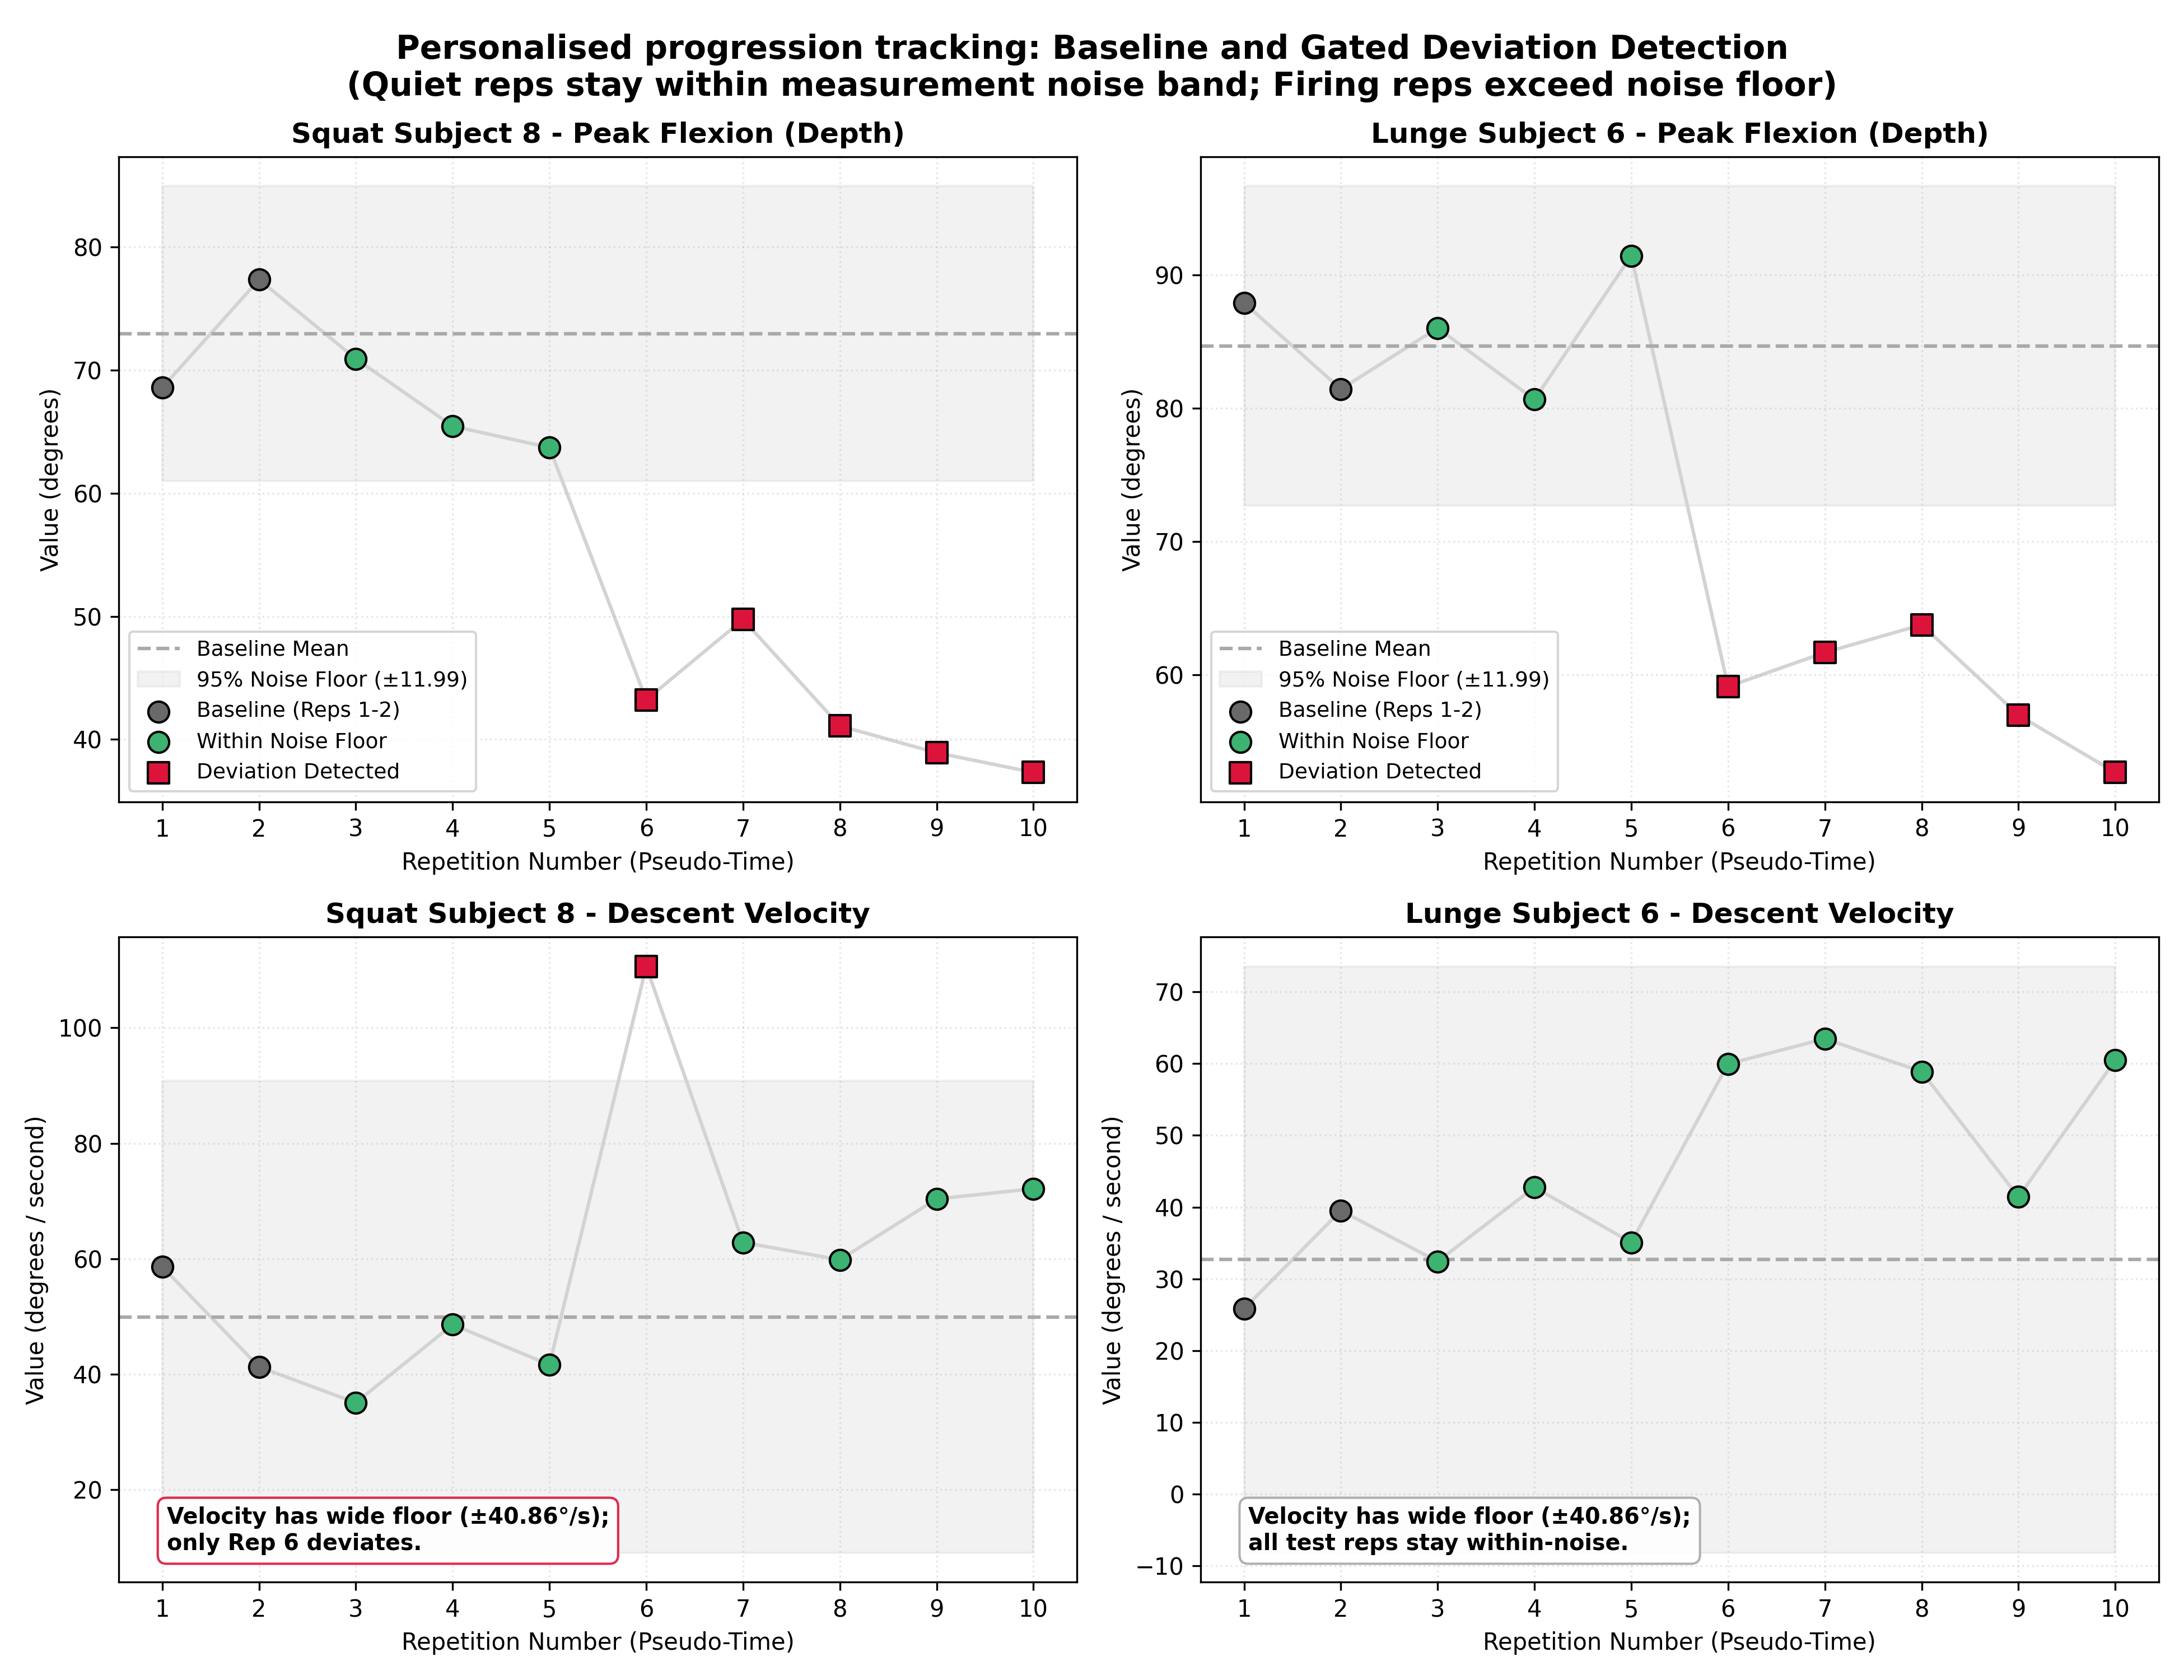
\includegraphics[width=0.95\textwidth]{fig9_1_baseline.png}
  \caption{Personalised Kinematic Progression Tracking with Uncertainty Gating. Each subject's running baseline mean and uncertainty-gated update windows are shown for peak flexion across sequential sessions.}
  \label{fig:baseline-tracking}
\end{figure}

\chapter{Rule-Based Screening Layer}
\label{ch:screening}

% SOURCE: results_screening_layer_v2.md
% STATUS: converted from markdown
% NOTE: [source:] tags stripped per ASSEMBLY_PLAN.md (harvested to appF)


This chapter presents the design, implementation, and verification of the rule-based screening layer (Step 10 of the biomechanical processing pipeline). While lower pipeline layers track raw joint coordinate data and calculate kinematics, clinical application requires interpreting these measurements into structured screening decisions. This chapter details a screening layer that converts joint angle deviations into named screening flags representing known, literature-grounded kinematic compensation patterns.



\section{Purpose and Core Deliverable Framing}
\label{sec:10-1-purpose-and-core-deliverable-framing}


The rule-based screening layer represents Step 10 of the primary pipeline architecture and serves as a core \textbf{Track A deliverable}. This distinguishes it from Track B architectural demonstrations (such as the digital twin sequence models), establishing it as the primary functional component of the screening system.

The primary purpose of this layer is to act as the transparent decision-making foundation of the clinical screening tool. It ingests kinematics (joint angles, ranges of motion, and velocities) and outputs a binary screening status (\texttt{SCREENING\_POSITIVE} or \texttt{NOT\_FLAGGED}) along with the specific list of rules triggered. Because screening checks are structured as deterministic, explicit logical statements, this layer remains completely transparent. This transparency is essential because it forms the exact decision layer that the subsequent Counterfactual Explainable AI (XAI) component (Step 11) is designed to explain, providing clinical users with clear mathematical justifications for every screening outcome.



\section{Critical Distinction: Screening vs. Tracking}
\label{sec:10-2-critical-distinction-screening-vs-tracking}


It is essential to distinguish this screening layer (Step 10) from the personalised tracking baselines (Chapters 9 and 11):
\begin{itemize}
  \item \textbf{Generic Tracking (Chapters 9 and 11)}: Evaluates a generic mathematical question: \textit{"Has this repetition shifted from the subject's reference by an amount exceeding measurement uncertainty?"}. This check is direction-agnostic and biomechanically blind; it simply flags any statistically significant signal change as a generic deviation.
  \item \textbf{Named-Rule Screening (Chapter 10)}: Ingests raw deviations detected by the tracking engine and maps them to \textbf{Named Screening Rules} (\texttt{EXCESS\_DEPTH}, \texttt{EXCESS\_ROM}, and \texttt{EXCESS\_VELOCITY}) with direction-specific thresholds. It evaluates: \textit{"Does this deviation match a known kinematic pattern associated with elevated injury risk or technique compensation?"}.
\end{itemize}

Tracking asks if something changed; screening asks if that change represents a specific, predefined movement deviation.



\section{Screening Modality Choice (Option B)}
\label{sec:10-3-screening-modality-choice-option-b}


Two primary modalities can evaluate joint kinematics in markerless pose estimation:
\begin{enumerate}
  \item \textbf{Option A (Fixed Population Thresholds)}: Gating joint values against absolute, cohort-wide normal values (e.g., flagging any squat where knee flexion exceeds $60^\circ$).
  \item \textbf{Option B (Personalised-Deviation Screening)}: Gating deviations against the subject's own baseline mean plus the validated measurement noise floor.
\end{enumerate}

We selected \textbf{Option B (Personalised-Deviation Screening)} and rejected Option A. Monocular pose estimation is subject to systematic projection bias (overestimation or underestimation) caused by the angle between the subject's sagittal plane and the camera's optical axis. Because this perspective angle is constant within a single subject's testing session, the resulting projection bias is also constant. By calculating deviations relative to the subject's session baseline, this systematic projection bias is mathematically cancelled:
\begin{equation}
  \Delta_i = |x_{\text{test}} - \mu_{\text{base}}| = |(x_{\text{true}} + \text{bias}) - (\mu_{\text{true}} + \text{bias})| = |x_{\text{true}} - \mu_{\text{true}}|
  \label{eq:disp1}
\end{equation}

This makes Option B highly robust to camera perspective offsets. In contrast, Option A would false-alarm or fail to detect deviations because perspective offsets vary unpredictably between subjects and camera setups, rendering universal absolute thresholds unviable for monocular video screening.



\section{Rules Definition and Cohort-Level Grounding}
\label{sec:10-4-rules-definition-and-cohort-level-grounding}


Sagittal knee joint angles represent included angles between thigh and shank segments ($\approx 180^\circ$ = full extension; smaller angles = deeper flexion). Comparing correct and incorrect distributions in the \texttt{REHAB24-6} squat ($n=98$) and lunge ($n=61$) cohorts grounds the direction of each rule:

\subsection{The Three Named Screening Rules}
\label{sec:10-4-1-the-three-named-screening-rules}

\begin{enumerate}
  \item \textbf{Peak Knee Flexion (\texttt{EXCESS\_DEPTH})}:
\end{enumerate}
\textit{   }Squat Cohort*: Correct mean = $60.85^\circ \pm 12.72^\circ$; Incorrect mean = $41.14^\circ \pm 6.20^\circ$ ($d = +1.7306$).
\textit{   }Lunge Cohort*: Correct mean = $89.66^\circ \pm 8.33^\circ$; Incorrect mean = $68.03^\circ \pm 15.11^\circ$ ($d = 1.6904$).
\textit{   }Biomechanical Grounding*: Incorrect repetitions exhibit smaller joint angles, representing a shift toward excessive flexion depth (mean shifts: $-19.71^\circ$ for squats, $-21.63^\circ$ for lunges). The \textbf{EXCESS\_DEPTH} rule fires when knee flexion angle drops below baseline minus noise floor:
\begin{equation}
  x_{\text{peak}} < \mu_{\text{base}, \text{peak}} - NF_{\text{peak}}
  \label{eq:disp2}
\end{equation}
\begin{enumerate}
  \item \textbf{Range of Motion (\texttt{EXCESS\_ROM})}:
\end{enumerate}
\textit{   }Squat Cohort*: Correct mean = $111.19^\circ \pm 18.06^\circ$; Incorrect mean = $134.31^\circ \pm 7.23^\circ$ ($d = -1.4484$).
\textit{   }Lunge Cohort*: Correct mean = $59.02^\circ \pm 20.94^\circ$; Incorrect mean = $90.30^\circ \pm 27.00^\circ$ ($d = -1.2653$).
\textit{   }Biomechanical Grounding*: Excessive depth causes incorrect repetitions to cover greater joint excursion (mean shifts: $+23.13^\circ$ for squats, $+31.28^\circ$ for lunges). The \textbf{EXCESS\_ROM} rule fires when joint excursion exceeds baseline plus noise floor:
\begin{equation}
  x_{\text{rom}} > \mu_{\text{base}, \text{rom}} + NF_{\text{rom}}
  \label{eq:disp3}
\end{equation}
\begin{enumerate}
  \item \textbf{Descent Velocity (\texttt{EXCESS\_VELOCITY})}:
\end{enumerate}
\textit{   }Squat Cohort*: Correct mean = $66.94^\circ/\text{s} \pm 22.24^\circ/\text{s}$; Incorrect mean = $83.14^\circ/\text{s} \pm 16.22^\circ/\text{s}$ (shift: $+16.20^\circ/\text{s}$).
\textit{   }Lunge Cohort*: Correct mean = $30.39^\circ/\text{s} \pm 8.26^\circ/\text{s}$; Incorrect mean = $52.64^\circ/\text{s} \pm 24.04^\circ/\text{s}$ (shift: $+22.25^\circ/\text{s}$).
\textit{   }Biomechanical Grounding*: Incorrect repetitions exhibit faster eccentric descent. The \textbf{EXCESS\_VELOCITY} rule fires when descent speed exceeds baseline plus noise floor:
\begin{equation}
  x_{\text{velocity}} > \mu_{\text{base}, \text{velocity}} + NF_{\text{velocity}}
  \label{eq:disp4}
\end{equation}

It is critical to emphasize that these thresholds are screening heuristics derived from empirical distributions, not validated clinical diagnostic cut-offs.

\subsection{Applied Noise Floors}
\label{sec:10-4-2-applied-noise-floors}

Gating noise floors ($NF_i$) transferred from Chapter 8 ground-truth validation are:
\begin{itemize}
  \item $NF_{\text{peak}} = \mathbf{11.99^\circ}$
  \item $NF_{\text{rom}} = \mathbf{23.17^\circ}$
  \item $NF_{\text{velocity}} = \mathbf{40.86^\circ/\text{s}}$
\end{itemize}



\section{Applied Results}
\label{sec:10-5-applied-results}


The screening rules were executed on Squat Subject 8 (\texttt{PM\_113}) and Lunge Subject 6 (\texttt{PM\_104}) from \texttt{REHAB24-6}.

\subsection{Squat Screening Results (Subject \texttt{PM\_113})}
\label{sec:10-5-1-squat-screening-results-subject-texttt-pm-113}

\begin{itemize}
  \item \textbf{Baseline Means (Reps 1–2)}: Peak flexion = \textbf{$72.98^\circ$}, ROM = \textbf{$105.50^\circ$}, descent velocity = \textbf{$49.94^\circ/\text{s}$}.
  \item \textbf{Gating Thresholds}: \texttt{EXCESS\_DEPTH} $< \mathbf{60.99^\circ}$ ($72.98^\circ - 11.99^\circ$); \texttt{EXCESS\_ROM} $> \mathbf{128.67^\circ}$ ($105.50^\circ + 23.17^\circ$); \texttt{EXCESS\_VELOCITY} $> \mathbf{90.80^\circ/\text{s}}$ ($49.94^\circ/\text{s} + 40.86^\circ/\text{s}$).
  \item \textbf{Quiet-Test Reps (Reps 3–5)}: Correct repetitions stayed within noise limits, returning \textbf{\texttt{NOT\_FLAGGED}}.
  \item \textbf{Firing-Test Reps (Reps 6–10)}: All five incorrect repetitions returned \textbf{\texttt{SCREENING\_POSITIVE}}:
\end{itemize}
\textit{   }Repetition 6*: Peak flexion $43.22^\circ$ (margin: \textbf{$17.77^\circ$}), ROM $136.50^\circ$ (margin: \textbf{$7.83^\circ$}), velocity $110.62^\circ/\text{s}$ (margin: \textbf{$19.82^\circ/\text{s}$}). Fired: \texttt{["EXCESS\_DEPTH", "EXCESS\_VELOCITY", "EXCESS\_ROM"]}.
\textit{   }Repetitions 7–10*: Flexion margins ranged from \textbf{$11.24^\circ$ to $23.67^\circ$}; ROM margins ranged from \textbf{$1.18^\circ$ to $13.54^\circ$}. Fired: \texttt{["EXCESS\_DEPTH", "EXCESS\_ROM"]}.

\subsection{Lunge Screening Results (Subject \texttt{PM\_104})}
\label{sec:10-5-2-lunge-screening-results-subject-texttt-pm-104}

\begin{itemize}
  \item \textbf{Baseline Means (Reps 1–2)}: Peak flexion = \textbf{$84.66^\circ$}, ROM = \textbf{$76.78^\circ$}, velocity = \textbf{$32.68^\circ/\text{s}$}.
  \item \textbf{Gating Thresholds}: \texttt{EXCESS\_DEPTH} $< \mathbf{72.68^\circ}$; \texttt{EXCESS\_ROM} $> \mathbf{99.95^\circ}$; \texttt{EXCESS\_VELOCITY} $> \mathbf{73.54^\circ/\text{s}}$.
  \item \textbf{Quiet-Test Reps (Reps 3–5)}: Returned \textbf{\texttt{NOT\_FLAGGED}}.
  \item \textbf{Firing-Test Reps (Reps 6–10)}: All incorrect reps returned \textbf{\texttt{SCREENING\_POSITIVE}}, triggering \texttt{["EXCESS\_DEPTH", "EXCESS\_ROM"]}. Peak flexion margins ranged from \textbf{$8.92^\circ$ to $19.99^\circ$}; ROM margins ranged from \textbf{$7.65^\circ$ to $21.85^\circ$}. Velocity stayed within noise floor ($73.54^\circ/\text{s}$), so it did not fire.
\end{itemize}

\subsection{Ground Truth Alignment Note}
\label{sec:10-5-3-ground-truth-alignment-note}

Alignment with dataset ground-truth labels (100\% agreement across test reps) represents a coincidental validation check using the dataset's labelling scheme. It does \textbf{not} indicate that the screening layer classifies "correctness" or issues form quality verdicts. The screening layer's operational role is strictly to detect and report kinematic deviations exceeding camera noise, not to judge performance quality.



\section{Boundaries and What This Layer Does NOT Claim}
\label{sec:10-6-boundaries-and-what-this-layer-does-not-claim}


To maintain scientific integrity and align with screening scope across this dissertation:
\begin{itemize}
  \item \textbf{No Diagnostic Verdicts}: Screening flags (e.g., \texttt{SCREENING\_POSITIVE}) are kinematic classifications representing baseline shifts, not clinical or medical diagnoses.
  \item \textbf{No Clinical Cut-Offs}: Thresholds (such as $\pm 11.99^\circ$) are camera-uncertainty heuristics derived from empirical distributions, not validated clinical diagnostic thresholds.
  \item \textbf{Not a Trained ML Model}: The layer uses no machine learning weights or neural networks. It is a deterministic, rule-based logic gate, fully explainable by construction.
  \item \textbf{No Injury Forecasting}: The layer detects active movement deviations; it does not forecast future injury likelihood or compute clinical risk scores.
\end{itemize}
\chapter{Biomechanical Digital Twin}
\label{ch:twin}

% SOURCE: results_digital_twin_v2.md
% STATUS: converted from markdown
% NOTE: [source:] tags stripped per ASSEMBLY_PLAN.md (harvested to appF)


This chapter presents the design and demonstration of a continuously-updating personalised "Digital Twin" framework. Static baseline references (Chapter 9) establish a fixed movement template from early repetitions. However, in clinical rehabilitation and athletic monitoring, movement patterns evolve dynamically due to warm-up effects, fatigue, or recovery. To capture these shifts, a digital twin must update its reference state continuously. We describe an architecture that applies a conditional update rule: the twin absorbs repetitions that fall within the camera's validated noise floor, while rejecting deviant trials to prevent baseline contamination.



\section{Purpose and Design Motivation}
\label{sec:11-1-purpose-and-design-motivation}


Unlike the static personalised baseline (Chapter 9), which evaluates joint angle deviations relative to a fixed early-session template, a clinical digital twin must accommodate natural movement drift. An athlete's kinematics shift over time due to warm-up effects, muscular fatigue, learning adaptations, or clinical recovery.

The primary objective of this chapter is to demonstrate an architectural extension of the personalised baseline: a continuous-update "Digital Twin". The twin maintains a rolling statistical reference profile of the user's active kinematics. When a new repetition is performed, the twin gates it against the active reference using the Chapter 8 validated projection noise floor. To ensure stability, the twin applies a \textbf{conditional update rule}: it incorporates the repetition into the reference mean if the trial is within the noise floor, but rejects the update if a deviation is detected, preventing the baseline from being corrupted by isolated technique breakdowns.

\subsection{Architectural Constraints and Scope}
\label{sec:11-1-1-architectural-constraints-and-scope}

To align with the screening scope across this dissertation:
\begin{enumerate}
  \item \textbf{Non-Predictive}: The twin does not forecast future movement trajectories, performance, or injury risk; it characterises the active reference state.
  \item \textbf{No Learned Parameters}: The update mechanism is an arithmetic running mean without machine learning weights, training rates, or state decay.
  \item \textbf{Pseudo-Session Axis}: Consistent with Chapter 9, within-session repetition order forms sequential \textbf{pseudo-sessions}. True longitudinal multi-session tracking across days is deferred to future work.
\end{enumerate}



\section{Continuous-Update Mechanism}
\label{sec:11-2-continuous-update-mechanism}


The digital twin state for biomarker $i$ at time step $t$ consists of a running reference mean ($\mu_{t, i}$), sample size ($N_{t, i}$), descriptive standard deviation ($SD_{t, i}$), and fixed validated noise floor ($NF_i = 1.96 \times SD_{\text{proj}, i}$) transferred from Chapter 8.

\subsection{Mathematical Conditional Update Rules}
\label{sec:11-2-1-mathematical-conditional-update-rules}

When a new repetition $x_{t+1, i}$ is ingested, its absolute deviation ($\Delta_i = |x_{t+1, i} - \mu_{t, i}|$) from the active reference mean is evaluated:
\begin{itemize}
  \item \textbf{\texttt{WITHIN-NOISE} Update ($\Delta_i \le NF_i$)}: The repetition reflects normal variation. The twin updates the running mean incrementally:
\begin{equation}
  \mu_{t+1, i} = \frac{N_{t, i} \cdot \mu_{t, i} + x_{t+1, i}}{N_{t, i} + 1}, \quad N_{t+1, i} = N_{t, i} + 1
  \label{eq:disp1}
\end{equation}
  \item \textbf{\texttt{DEVIATION DETECTED} Rejection ($\Delta_i > NF_i$)}: The repetition represents a significant kinematic shift. To prevent reference contamination, the repetition is \textbf{excluded} from the update:
\begin{equation}
  \mu_{t+1, i} = \mu_{t, i}, \quad N_{t+1, i} = N_{t, i}
  \label{eq:disp2}
\end{equation}
\end{itemize}

This conditional update rule ensures self-stabilization: the reference tracks slow, normal kinematic shifts while locking flat during movement faults without allowing them to drift the baseline.



\section{Results -- Reference Evolution and Locking Flat}
\label{sec:11-3-results-reference-evolution-and-locking-flat}


The continuous-update mechanism was validated across three sequential pseudo-sessions using 10-repetition sequences from Squat Subject 8 (\texttt{PM\_113}) and Lunge Subject 6 (\texttt{PM\_104}): Initialization (Reps 1–2, $\mu_0$), Normal Practice (Reps 3–5), and Deviated Practice (Reps 6–10).

\subsection{Squat Demonstration (Subject \texttt{PM\_113})}
\label{sec:11-3-1-squat-demonstration-subject-texttt-pm-113}

Subject \texttt{PM\_113} performed 5 correct squats followed by 5 restricted-depth squats:
\begin{itemize}
  \item \textbf{Initialization (Reps 1–2)}: Established initial reference mean peak flexion at \textbf{$72.98^\circ$}.
  \item \textbf{Reference Evolution (Reps 3–5)}: Each rep fell within the peak flexion noise floor ($\pm 11.99^\circ$), updating the running mean from $72.98^\circ$ to \textbf{$72.30^\circ$} (Rep 3), \textbf{$70.59^\circ$} (Rep 4), and \textbf{$69.21^\circ$} (Rep 5).
  \item \textbf{Reference Locking Flat (Reps 6–10)}: Rep 6 peak flexion dropped to $43.22^\circ$ (deviation: \textbf{$25.99^\circ > \pm 11.99^\circ$}), triggering \texttt{DEVIATION DETECTED}. Across Reps 6–10, peak flexion deltas ranged from \textbf{$19.47^\circ$ to $31.90^\circ$}, causing the peak flexion reference to lock flat at \textbf{$69.21^\circ$}.
\end{itemize}

\subsection{Lunge Demonstration (Subject \texttt{PM\_104})}
\label{sec:11-3-2-lunge-demonstration-subject-texttt-pm-104}

Subject \texttt{PM\_104} performed 5 correct lunges followed by 5 restricted-depth lunges:
\begin{itemize}
  \item \textbf{Initialization (Reps 1–2)}: Established initial reference mean peak flexion at \textbf{$84.66^\circ$}.
  \item \textbf{Reference Evolution (Reps 3–5)}: Correct reps updated the reference mean to \textbf{$85.11^\circ$} (Rep 3), \textbf{$84.00^\circ$} (Rep 4), and \textbf{$85.48^\circ$} (Rep 5).
  \item \textbf{Reference Locking Flat (Reps 6–10)}: Restricted-depth lunges yielded peak flexion deviations relative to active reference ($85.48^\circ$) ranging from \textbf{$20.91^\circ$ to $32.80^\circ > \pm 11.99^\circ$}. Exceeding the noise floor, all five reps were excluded, locking the reference flat at \textbf{$85.48^\circ$}.
\end{itemize}

The 95\% noise-floor band ($NF_i$) tracks the evolving reference dynamically across Pseudo-Session 2 before locking during Pseudo-Session 3.



\section{Per-Biomarker Update Independence}
\label{sec:11-4-per-biomarker-update-independence}


A key design feature is that update logic operates independently for each biomarker on the same repetition. Joint angles, ranges of motion, and velocities represent distinct kinematic dimensions and can exist in different gating states during a single trial.

This is demonstrated on \textbf{Repetition 7} of Squat Subject \texttt{PM\_113}:
\begin{itemize}
  \item \textbf{Peak Flexion (\texttt{DEVIATION DETECTED})}: Peak flexion ($49.75^\circ$) deviated by $19.47^\circ > \pm 11.99^\circ$ floor; update withheld, reference locked at \textbf{$69.21^\circ$}.
  \item \textbf{Range of Motion (\texttt{WITHIN-NOISE})}: ROM ($129.84^\circ$) deviated by $20.36^\circ \le \pm 23.17^\circ$ floor; reference updated from $109.48^\circ$ to \textbf{$112.88^\circ$}.
  \item \textbf{Descent Velocity (\texttt{WITHIN-NOISE})}: Velocity ($62.83^\circ/\text{s}$) deviated by $17.79^\circ/\text{s} \le \pm 40.86^\circ/\text{s}$ floor; reference updated from $45.03^\circ/\text{s}$ to \textbf{$48.00^\circ/\text{s}$}.
\end{itemize}

Rather than rejecting the entire trial, the twin selectively updates valid biomarker components, maximizing data utilization while isolating specific deviations.



\section{Explainable Exclusion and Epistemic Humility}
\label{sec:11-5-explainable-exclusion-and-epistemic-humility}


When excluding a repetition from the reference update, the twin generates a transparent, measurement-based explanation. During Squat Subject \texttt{PM\_113} Repetition 6, the framework generated:

\begin{quote}
\textit{"Rep 6 deviated from your baseline beyond validated measurement uncertainty (on biomarker peak flexion). The twin does not update the reference from this rep, because from a single observation it cannot distinguish a transient fluctuation from a genuine sustained change — that distinction would require the deviation to persist across multiple sessions."}
\end{quote}

This design contrasts with black-box classification models. Rather than declaring a repetition "bad" or issuing a clinical verdict, the message reflects \textbf{epistemic humility}: it attributes withholding to single-observation ambiguity, references camera measurement uncertainty logic, and transparently communicates system limits.



\section{Transient-vs-Sustained Adaptation (Future Work)}
\label{sec:11-6-transient-vs-sustained-adaptation-future-work}


The explainable exclusion message directly motivates future research on continuous update architectures:
\begin{itemize}
  \item \textbf{Transient Fluctuations}: Restricted-depth reps in this study represent temporary within-session deviations. The twin correctly isolates these faults and keeps the baseline stable.
  \item \textbf{Sustained Adaptation}: If an athlete permanently alters movement strategy (clinical recovery or new technique), rejecting all future reps would lock the baseline indefinitely.
  \item \textbf{Future Longitudinal Persistence}: A deployed longitudinal twin requires multi-session persistence logic: if a deviation persists across multiple real sessions, the twin must absorb the shift, adapting the reference mean to the new movement template.
\end{itemize}



\section{What This Framework Does NOT Claim}
\label{sec:11-7-what-this-framework-does-not-claim}


To maintain scientific integrity and align with screening scope:
\begin{itemize}
  \item \textbf{No Predictive Forecasting}: Does not forecast future movement parameters, fatigue, or recovery.
  \item \textbf{No Injury Risk Scoring}: Does not calculate injury risk indices or likelihoods.
  \item \textbf{No Correctness Verdicts}: Flags baseline deviations, not correctness. Cohort correctness labels serve only to validate rejection logic.
  \item \textbf{Not a Deployed Clinical System}: Serves as a software architectural prototype.
\end{itemize}



\section{Figures and Provenance}
\label{sec:11-8-figures}
The following publication-ready figure supports this chapter.

\begin{figure}[htbp]
  \centering
  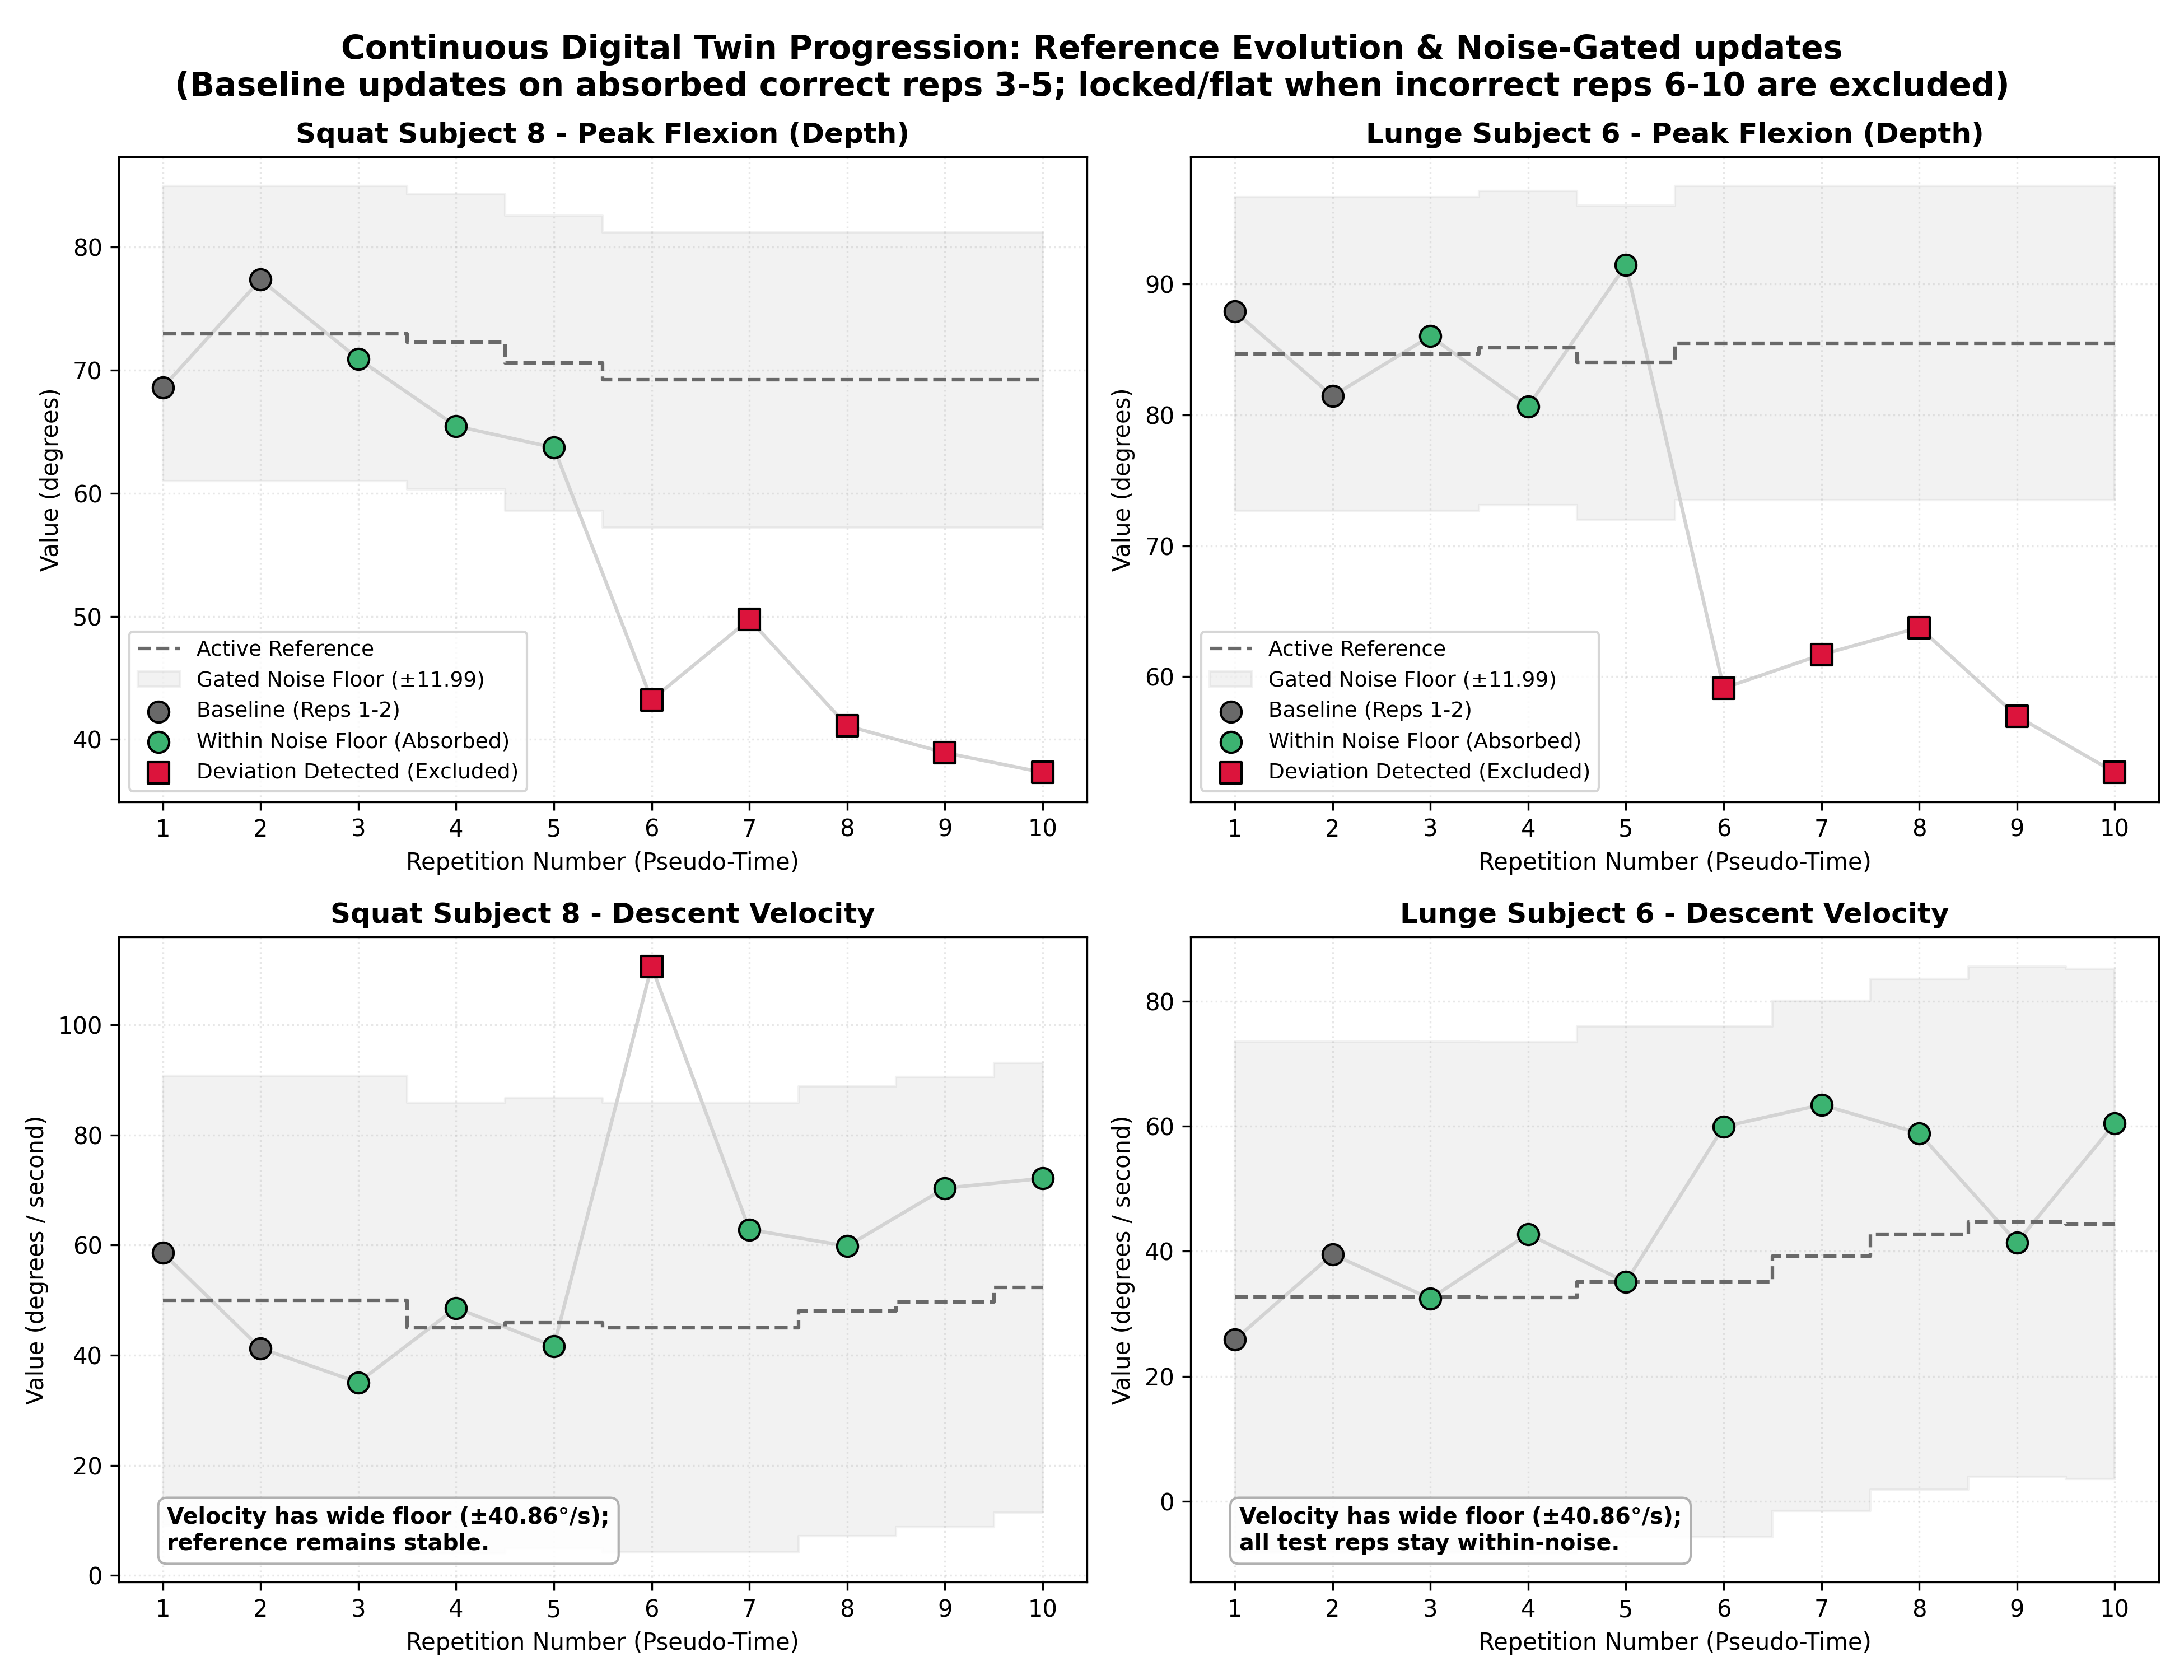
\includegraphics[width=0.95\textwidth]{fig11_1_twin.png}
  \caption{Continuously-Updating Personalised Digital Twin with Conditional Update Gating. The twin state (running mean $\pm$ noise floor) updates only when new observations fall within the validated measurement uncertainty window, ensuring biological drift is distinguished from measurement noise.}
  \label{fig:digital-twin}
\end{figure}

\chapter{Counterfactual Explainable AI (XAI)}
\label{ch:xai}

% SOURCE: results_xai_v2.md
% STATUS: converted from markdown
% NOTE: [source:] tags stripped per ASSEMBLY_PLAN.md (harvested to appF)


This chapter presents the design, implementation, and verification of the counterfactual Explainable AI (XAI) layer (Step 11 of the biomechanical processing pipeline). Biomechanical screening tools must not only identify movement deviations but also communicate their decisions transparently to clinical users. This chapter details a counterfactual explanation component that defines the exact physical joint boundaries required to clear active screening flags.



\section{Purpose and Step 11 Novelty Framing}
\label{sec:12-1-purpose-and-step-11-novelty-framing}


The counterfactual XAI layer represents Step 11 of the primary pipeline architecture and constitutes \textbf{Novelty Contribution \protect\#4} of this dissertation.

The primary purpose of this layer is to translate the binary decisions of the Step 10 screening layer into clinical explanations. For any repetition flagged as \texttt{SCREENING\_POSITIVE}, the XAI layer computes a counterfactual explanation: a statement defining the exact kinematic conditions under which the screening flags would \textit{not} have fired. Rather than providing abstract, post-hoc feature importance scores (which show that a biomarker was "important" without defining how it must change), counterfactuals provide concrete, physical joint values. This bridges raw joint coordinate tracking and clinical decision-making, helping practitioners understand the precise boundary between a normal baseline pattern and a detected deviation.



\section{Research Origin and SHAP/LIME Deprecation}
\label{sec:12-2-research-origin-and-shap-lime-deprecation}


The design of the explainability component underwent a major methodological shift during development:
\begin{itemize}
  \item \textbf{Initial Scaffold \& Deprecation}: The original workspace structure featured placeholder directories (\texttt{8\_xai/}) for model-agnostic post-hoc explanation frameworks, specifically SHAP (SHapley Additive exPlanations) and LIME (Local Interpretable Model-agnostic Explanations). However, SHAP and LIME are approximation tools designed for black-box machine learning models (such as deep neural networks) by perturbing inputs locally to reconstruct decision boundaries.
  \item \textbf{Pipeline Realignment}: Because the Step 10 screening layer is a deterministic, transparent logic gate with explicit thresholds, fitting a post-hoc surrogate model introduces unnecessary approximation error and explanation infidelity. Consequently, SHAP and LIME were deprecated in favor of a direct, exact counterfactual engine that calculates margins directly from the pipeline's active thresholds.
\end{itemize}



\section{Faithfulness by Construction}
\label{sec:12-3-faithfulness-by-construction}


The defining advantage of the direct counterfactual explanation layer is \textbf{faithfulness by construction}.

In black-box explanation methods, there is a constant trade-off between interpretability and faithfulness because the local surrogate model is only an approximation of the primary model's behavior. In this framework, the decision rules defined in Step 10 \textit{are} the decision boundaries. The counterfactual engine calculates the deviation margin ($M_i$) directly from the active threshold ($T_i$) and the measured joint value ($x_i$):
\begin{equation}
  M_{\text{depth}} = T_{\text{depth}} - x_{\text{peak}}
  \label{eq:disp1}
\end{equation}
\begin{equation}
  M_{\text{rom}} = x_{\text{rom}} - T_{\text{rom}}
  \label{eq:disp2}
\end{equation}
\begin{equation}
  M_{\text{velocity}} = x_{\text{velocity}} - T_{\text{velocity}}
  \label{eq:disp3}
\end{equation}

Because explanations are derived from these exact algebraic margins, they exhibit \textbf{zero approximation error}. Unlike local surrogate models that can produce unstable explanations across neighboring samples, this glass-box engine is guaranteed to be a mathematically perfect representation of the underlying screening decision. This faithfulness by construction represents a major methodological contribution of the Track A architecture.



\section{Counterfactual Templates and Wording Direction}
\label{sec:12-4-counterfactual-templates-and-wording-direction}


The XAI layer utilizes predefined wording templates to generate explanations. Because knee angles use the included-angle convention (extension $\approx 180^\circ$, smaller angles = deeper flexion), template directions are verified to prevent clinical contradictions:

\begin{enumerate}
  \item \textbf{EXCESS\_DEPTH (Peak Knee Flexion)}:
\end{enumerate}
*   Fires if peak included angle $x_{\text{peak}} < T_{\text{depth}}$ (smaller knee angle, deeper bend).
\textit{   }Counterfactual template*: \texttt{"Flagged EXCESS\_DEPTH because peak knee flexion joint angle (x\_peak°) was M\_depth° below the active baseline threshold (T\_depth°). Had the peak flexion angle been at least T\_depth° (representing a shallower bend of M\_depth° less depth), the EXCESS\_DEPTH flag would not have fired."}.
\textit{   }Direction Verification*: Since $T_{\text{depth}}$ is algebraically larger than $x_{\text{peak}}$, requiring the angle to be "at least $T_{\text{depth}}$" physically corresponds to a shallower flexion bend.
\begin{enumerate}
  \item \textbf{EXCESS\_ROM (Range of Motion Excursion)}:
\end{enumerate}
*   Fires if range of motion $x_{\text{rom}} > T_{\text{rom}}$ (larger excursion).
\textit{   }Counterfactual template*: \texttt{"Flagged EXCESS\_ROM because knee range of motion (x\_rom°) was M\_rom° above the active baseline threshold (T\_rom°). Had the range of motion been no more than T\_rom° (representing a restricted excursion of M\_rom° less joint travel), the EXCESS\_ROM flag would not have fired."}.
\begin{enumerate}
  \item \textbf{EXCESS\_VELOCITY (Eccentric Descent Velocity)}:
\end{enumerate}
*   Fires if descent velocity $x_{\text{velocity}} > T_{\text{velocity}}$ (faster speed).
\textit{   }Counterfactual template*: \texttt{"Flagged EXCESS\_VELOCITY because descent joint velocity (x\_velocity°/s) was M\_velocity°/s above the active baseline threshold (T\_velocity°/s). Had the descent velocity been no more than T\_velocity°/s (representing a slower movement of M\_velocity°/s less speed), the EXCESS\_VELOCITY flag would not have fired."}.

Explanations are phrased \textbf{descriptively} (describing the mathematical boundary condition that would satisfy the gate), never \textbf{prescriptively} (instructing the athlete on how they must perform the movement).



\section{Minimal Kinematic Intervention (MKI)}
\label{sec:12-5-minimal-kinematic-intervention-mki}


When a repetition triggers multiple screening rules, joint parameter adjustments are physically coupled. For example, peak flexion depth and joint range of motion (ROM) are structurally linked: restricting a squat's depth simultaneously restricts its range of motion.

To account for this coupling, the XAI layer implements a \textbf{Minimal Kinematic Intervention (MKI)} arithmetic. Under the biomechanical assumption that range of motion scales directly with peak flexion depth (assuming a constant standing extension start point, $x_{\text{rom}} \approx x_{\text{extension}} - x_{\text{peak}}$), the MKI computes the maximum of the two required peak flexion changes:
\begin{equation}
  \Delta \theta_{\text{MKI}} = \max(M_{\text{depth}}, M_{\text{rom}})
  \label{eq:disp4}
\end{equation}

The MKI output consolidates coupled explanations into a single descriptive statement defining the minimum flexion adjustment that satisfies both rule conditions simultaneously, avoiding contradictory multi-variable recommendations. Independent biomarkers (such as descent velocity) are appended as a separate condition in a set of requirements:
\begin{equation}
  \text{MKI Statement} = \left\{ \Delta \theta_{\text{MKI}} \text{ shallower peak flexion} \right\} \cup \left\{ M_{\text{velocity}} \text{ slower joint speed} \right\}
  \label{eq:disp5}
\end{equation}

This MKI coupling assumption is an illustrative simplification for demonstrating multi-variable explanations, rather than an absolute biomechanical law.



\section{Uncertainty-Aware Confidence Grading}
\label{sec:12-6-uncertainty-aware-confidence-grading}


To prevent clinical users from over-interpreting minor tracking variations, counterfactual explanations incorporate Phase 7 validated camera noise floors to grade explanation confidence. Each deviation margin ($M_i$) is evaluated against a confidence buffer ($B_i = 0.5 \times NF_i$):
\begin{itemize}
  \item \textbf{\texttt{HIGH CONFIDENCE} ($M_i > B_i$)}: Margin is large enough to be clearly distinguished from monocular projection noise.
  \item \textbf{\texttt{LOW CONFIDENCE (Near Noise Floor)} ($M_i \le B_i$)}: Margin is close to uncertainty boundaries, appending a caution note:
\end{itemize}
> \textit{"Note: The deviation margin (M\_i) is close to the monocular camera's validated measurement uncertainty boundaries. This flag should be interpreted with caution as minor tracking fluctuations could have triggered it."}.

This confidence grading threads ground-truth optoelectronic validation (Chapter 6) through to XAI outputs.



\section{Applied Explanations Results}
\label{sec:12-7-applied-explanations-results}


Counterfactual explanations were executed on Squat Subject 8 (\texttt{PM\_113}) and Lunge Subject 6 (\texttt{PM\_104}) from \texttt{REHAB24-6}.

\subsection{Squat Worked Example: Subject \texttt{PM\_113} Repetition 6}
\label{sec:12-7-1-squat-worked-example-subject-texttt-pm-113-repetition-6}

Subject \texttt{PM\_113} Repetition 6 triggered \texttt{EXCESS\_DEPTH}, \texttt{EXCESS\_ROM}, and \texttt{EXCESS\_VELOCITY}. Active noise floors ($NF_{\text{peak}} = 11.99^\circ$, $NF_{\text{rom}} = 23.17^\circ$, $NF_{\text{velocity}} = 40.86^\circ/\text{s}$) defined confidence buffers of $5.99^\circ$, $11.58^\circ$, and $20.43^\circ/\text{s}$:
\begin{itemize}
  \item \textbf{\texttt{EXCESS\_DEPTH} Explanation}: Peak flexion angle was $43.22^\circ$ (threshold: $60.99^\circ$), margin \textbf{$17.77^\circ$} ($17.77^\circ > 5.99^\circ \rightarrow$ \textbf{\texttt{HIGH CONFIDENCE}}):
\end{itemize}
> \texttt{"Flagged EXCESS\_DEPTH because peak knee flexion joint angle (43.22°) was 17.77° below the active baseline threshold (60.99°). Had the peak flexion angle been at least 60.99° (representing a shallower bend of 17.77° less depth), the EXCESS\_DEPTH flag would not have fired."}.
\begin{itemize}
  \item \textbf{\texttt{EXCESS\_ROM} Explanation}: Range of motion was $136.50^\circ$ (threshold: $128.67^\circ$), margin \textbf{$7.83^\circ$} ($7.83^\circ \le 11.58^\circ \rightarrow$ \textbf{\texttt{LOW CONFIDENCE (Near Noise Floor)}}):
\end{itemize}
> \texttt{"Flagged EXCESS\_ROM because knee range of motion (136.50°) was 7.83° above the active baseline threshold (128.67°). Had the range of motion been no more than 128.67° (representing a restricted excursion of 7.83° less joint travel), the EXCESS\_ROM flag would not have fired. [Note: Near noise floor caution appended.]"}.
\begin{itemize}
  \item \textbf{\texttt{EXCESS\_VELOCITY} Explanation}: Descent velocity was $110.62^\circ/\text{s}$ (threshold: $90.80^\circ/\text{s}$), margin \textbf{$19.82^\circ/\text{s}$} ($19.82^\circ/\text{s} \le 20.43^\circ/\text{s} \rightarrow$ \textbf{\texttt{LOW CONFIDENCE (Near Noise Floor)}}).
  \item \textbf{Minimal Kinematic Intervention (MKI)}: Flexion adjustment was $\max(17.77^\circ, 7.83^\circ) = 17.77^\circ$. Velocity was independent ($19.82^\circ/\text{s}$). MKI rendered as:
\end{itemize}
> \texttt{"The screening flags would not have fired if peak knee flexion joint angle had been at least 17.77° shallower (which, assuming range of motion scales directly with peak flexion depth under a constant standing extension start point, would simultaneously restrict joint range of motion sufficiently to clear both the EXCESS\_DEPTH and EXCESS\_ROM flags) AND descent joint velocity had been at least 19.82°/s slower."}.

\subsection{Lunge Worked Example: Subject \texttt{PM\_104} Repetition 6}
\label{sec:12-7-2-lunge-worked-example-subject-texttt-pm-104-repetition-6}

Subject \texttt{PM\_104} Repetition 6 triggered \texttt{EXCESS\_DEPTH} and \texttt{EXCESS\_ROM}:
\begin{itemize}
  \item \textbf{\texttt{EXCESS\_DEPTH} Explanation}: Flexion angle $59.12^\circ$ (threshold: $72.68^\circ$), margin \textbf{$13.55^\circ$} (\textbf{\texttt{HIGH CONFIDENCE}}).
  \item \textbf{\texttt{EXCESS\_ROM} Explanation}: ROM $117.28^\circ$ (threshold: $99.95^\circ$), margin \textbf{$17.33^\circ$} ($17.33^\circ > 11.58^\circ \rightarrow$ \textbf{\texttt{HIGH CONFIDENCE}}).
  \item \textbf{Minimal Kinematic Intervention (MKI)}: Computed as $\max(13.55^\circ, 17.33^\circ) = 17.33^\circ$.
\end{itemize}
> \texttt{"The screening flags would not have fired if peak knee flexion joint angle had been at least 17.33° shallower (which, assuming range of motion scales directly with peak flexion depth under a constant standing extension start point, would simultaneously restrict joint range of motion sufficiently to clear both the EXCESS\_DEPTH and EXCESS\_ROM flags)."}.

Because the ROM margin ($17.33^\circ$) exceeded the peak flexion depth margin ($13.55^\circ$), max-coupling selected the larger constraint, clearing both rules simultaneously.

\subsection{Empirical Verification Summary}
\label{sec:12-7-3-empirical-verification-summary}

Faithfulness by construction was empirically confirmed by cross-checking every flagged repetition's rendered counterfactual margin against the screening layer's independently-computed threshold (\texttt{worked\_example\_screening.csv} vs \texttt{worked\_example\_explanations.json}). The complete side-by-side verification parameter table cross-checking raw values and rendered margins is presented in Appendix D (Table D.1).



\section{Boundaries and What This Layer Does NOT Claim}
\label{sec:12-8-boundaries-and-what-this-layer-does-not-claim}


To maintain scientific integrity and align with screening scope across this dissertation:
\begin{itemize}
  \item \textbf{Rule Explanations Only}: Explains rule-firing logic (why a flag was raised given biomarker values); does \textbf{NOT} explain injury causation, biomechanical mechanisms, or clinical outcomes.
  \item \textbf{No Diagnostics}: Does not provide clinical diagnostic interpretations or predict future joint injury.
  \item \textbf{No Prescriptive Training Advice}: Counterfactuals describe mathematical conditions required to clear flags; they do \textbf{not} recommend physical corrections or prescribe training interventions.
  \item \textbf{No Black-Box Approximations}: Does not explain neural networks or approximate black-box models (not SHAP/LIME); remains mathematically faithful to deterministic screening logic.
\end{itemize}
\chapter{Temporal Sequence Model}
\label{ch:temporal}

% SOURCE: results_temporal_model_v2.md
% STATUS: converted from markdown
% NOTE: [source:] tags stripped per ASSEMBLY_PLAN.md (harvested to appF)


This chapter presents the design, evaluation, and interpretation of temporal sequence modeling (Phase 12, Track B architectural demonstration). We examine whether within-repetition joint trajectory dynamics contain discriminative form screening information independent of, or superior to, static endpoint biomarkers. First, we define the research question and frame this evaluation as an empirical inquiry where null outcomes are pre-registered as scientifically informative. Second, we detail the Leave-One-Subject-Out (LOSO) cross-validation protocol and normalization schemes designed to prevent subject-identity leakage. Third, we present compiled sequence model results against naive and static endpoint baselines. Fourth, we interpret these findings under a pre-registered framework, concluding that static endpoints dominate at this cohort scale and diagnosing network overfitting. Finally, we outline an evidence-grounded roadmap for self-supervised pretraining and describe study limitations.



\section{Purpose and Research Question}
\label{sec:13-1-purpose-and-research-question}


The core research question evaluated in this chapter is: \textbf{Does modeling the within-repetition frame-by-frame joint-angle trajectory shape distinguish correct from incorrect repetitions beyond what is captured by static endpoint biomarkers?}

We distinguish this analysis along two structural axes:
\begin{itemize}
  \item \textbf{Within-Repetition Trajectory Shape}: The frame-by-frame geometric path of a single repetition resampled to a normalized time grid.
  \item \textbf{Across-Session Longitudinal Modeling}: Tracking parameters across multiple sessions over days or weeks (addressed via static baselines and digital twins in Chapters 9 and 11). This chapter is strictly restricted to within-repetition trajectory shape classification.
\end{itemize}

This evaluation is structured as a \textbf{Track B architectural demonstration}. Rather than optimizing a model to force a positive result, we treat this experiment as an empirical test of sequence modeling utility. Under this paradigm, a null or negative result (sequence shape adding no value) is pre-registered as a valuable, successful scientific finding. It provides empirical evidence demonstrating whether clinical screening layers can safely rely on transparent endpoint rules rather than complex deep sequence models.



\section{Experimental Design and Evaluation Rigour}
\label{sec:13-2-experimental-design-and-evaluation-rigour}


To isolate trajectory shape signals from confounding leakage pathways, we implemented a rigorous evaluation framework.

\subsection{Leave-One-Subject-Out (LOSO) Validation}
\label{sec:13-2-1-leave-one-subject-out-loso-validation}

Subject-identity leakage represents a major failure mode in small-cohort biomechanical modeling, where neural networks memorize subject-specific kinematic offsets rather than generalizable movement boundaries. To eliminate this confound, we utilized a strict \textbf{Leave-One-Subject-Out (LOSO) cross-validation} scheme across 9 folds for squats ($N=98$ reps) and 7 folds for lunges ($N=61$ reps). In each fold, all repetitions of a single subject were held out as the test set, guaranteeing zero subject data leakage into training splits.

\subsection{Temporal Standardization \& Anti-Leakage Normalization}
\label{sec:13-2-2-temporal-standardization-anti-leakage-normalization}

To decouple shape from repetition duration ($41\text{--}166$ frames), trajectories were linearly resampled to a fixed grid of \textbf{$T = 100$ points}. We evaluated models under two anti-leakage normalization schemes:
\begin{enumerate}
  \item \textbf{Scheme A (Offset Subtraction / Zero-Anchor)}: $\theta_{\text{offset}}(t) = \theta(t) - \theta(0)$, subtracting standing angle to neutralize perspective elevation while preserving ROM and maximum depth amplitude.
  \item \textbf{Scheme B (Min-Max Scaling / Pure Shape)}:scaling values strictly between $0.0$ and $1.0$ to strip all amplitude information, forcing classification based \textbf{solely} on time-dependent shape geometry.
\begin{equation}
  \theta_{\text{shape}}(t) = \frac{\theta(t) - \min(\theta)}{\max(\theta) - \min(\theta)}
  \label{eq:auto1}
\end{equation}
\end{enumerate}

\subsection{Models Compared and Pre-Registered Outcomes}
\label{sec:13-2-3-models-compared-and-pre-registered-outcomes}

Four models were evaluated on identical LOSO folds: (1) \textbf{Naive Baseline} (majority class guess); (2) \textbf{Endpoint Biomarker Baseline} (Logistic Regression on single biomarker \texttt{peak\_flexion\_deg}); (3) \textbf{Shape-Feature Baseline} (Logistic Regression on 6 handcrafted amplitude-invariant shape features such as duration ratio, velocity skewness, and concavity); and (4) \textbf{Model A LSTM} (miniature sequence network: $100 \times 1$ input, 8 hidden LSTM units, 4 dense units, heavy dropout and L2 regularization).

Crucially, three outcome scenarios were \textbf{pre-registered prior to training}:
\begin{itemize}
  \item \textbf{Outcome 1 (Shape Dynamics)}: LSTM $>$ Shape Baseline $>$ Naive \& Endpoint (sequence shape contains key independent signal).
  \item \textbf{Outcome 2 (Simple Geometry)}: Shape Baseline $\approx$ LSTM $>$ Naive \& Endpoint (shape adds low-order value, making deep LSTMs unnecessary).
  \item \textbf{Outcome 3 (Endpoint Dominance)}: Endpoint Baseline $\ge$ Shape Baseline $\approx$ LSTM (within-repetition shape details carry no discriminative value beyond static endpoints).
\end{itemize}



\section{Results}
\label{sec:13-3-results}


Global LOSO classification metrics are presented in Table 13.1. Per-fold results were consistent with this aggregate pattern across all held-out subjects; the full fold-by-fold table is presented in Appendix C.


\begin{table}[htbp]
\centering
\scriptsize
\setlength{\tabcolsep}{3pt}
\renewcommand{\arraystretch}{1.2}
\caption{Global Sequence Model Performance Metrics (LOSO CV)}
\label{tab:table-13-1-global-sequence-model-performance-metrics-loso-cv}
\begin{tabular}{@{}p{1.4cm} p{2.7cm} >{\centering\arraybackslash}p{1.4cm} >{\centering\arraybackslash}p{1.8cm} >{\centering\arraybackslash}p{2.0cm} >{\centering\arraybackslash}p{1.6cm} >{\centering\arraybackslash}p{1.6cm}@{}}
\hline
\textbf{Exercise} & \textbf{Normalization} & \textbf{Model} & \textbf{Accuracy} & \textbf{Balanced Acc} & \textbf{F1-Score} & \textbf{AUC-ROC} \\
\hline
Squat ($N=98$) & Scheme\_A (Offset Sub) & naive & $73.47\%$ & $50.00\%$ & $0.8471$ & $0.5000$ \\
 &  & peak & $81.63\%$ & $81.36\%$ & $0.8676$ & $0.9038$ \\
 &  & shape & $38.78\%$ & $33.76\%$ & $0.5161$ & $0.3531$ \\
 &  & lstm & $59.18\%$ & $53.79\%$ & $0.7015$ & $0.4931$ \\
 & Scheme\_B (Min-Max) & naive & $73.47\%$ & $50.00\%$ & $0.8471$ & $0.5000$ \\
 &  & peak & $81.63\%$ & $81.36\%$ & $0.8676$ & $0.9038$ \\
 &  & shape & $38.78\%$ & $33.76\%$ & $0.5161$ & $0.3531$ \\
 &  & lstm & $73.47\%$ & $50.00\%$ & $0.8471$ & $0.6050$ \\
Lunge ($N=61$) & Scheme\_A (Offset Sub) & naive & $59.02\%$ & $50.00\%$ & $0.0000$ & $0.5000$ \\
 &  & peak & $80.33\%$ & $81.50\%$ & $0.7857$ & $0.8289$ \\
 &  & shape & $57.38\%$ & $58.39\%$ & $0.5517$ & $0.5889$ \\
 &  & lstm & $54.10\%$ & $53.78\%$ & $0.4815$ & $0.5378$ \\
 & Scheme\_B (Min-Max) & naive & $59.02\%$ & $50.00\%$ & $0.0000$ & $0.5000$ \\
 &  & peak & $80.33\%$ & $81.50\%$ & $0.7857$ & $0.8289$ \\
 &  & shape & $57.38\%$ & $58.39\%$ & $0.5517$ & $0.5889$ \\
 &  & lstm & $42.62\%$ & $39.17\%$ & $0.2222$ & $0.4144$ \\
\hline
\end{tabular}
\end{table}

\subsection{Performance Analysis}
\label{sec:13-3-1-performance-analysis}

\begin{itemize}
  \item \textbf{Peak Flexion Dominance}: The single static peak flexion classifier outperformed all sequence models, achieving \textbf{$81.36\%$ Balanced Accuracy} on squats (AUC = $0.9038$) and \textbf{$81.50\%$ Balanced Accuracy} on lunges (AUC = $0.8289$).
  \item \textbf{LSTM Performance}: Under Scheme B (pure shape), the LSTM collapsed to the naive majority baseline ($50.00\%$ Balanced Accuracy on squats; $39.17\%$ on lunges). Under Scheme A (amplitude preserved), the LSTM achieved only $53.79\%$ (squats) and $53.78\%$ (lunges), performing barely above chance.
  \item \textbf{Sub-Chance Shape Baseline Artifact}: The squat shape baseline yielded a sub-chance balanced accuracy of $33.76\%$. Diagnostic checks confirmed this is a statistical artifact of class weighting on zero-signal noise: without class weighting, the model predicts the majority class ($49.31\%$ balanced accuracy). Class weighting shifts the boundary to minimize minority loss, causing heavy validation over-prediction on zero-signal noise and confirming trajectory shape contains no discriminative information.
\end{itemize}



\section{Interpretation and Overfitting Diagnostics}
\label{sec:13-4-interpretation-and-overfitting-diagnostics}


The empirical results conclusively confirm \textbf{Outcome 3 (Endpoint Dominance)}. Within-repetition trajectory shape, timing, and velocity profiles contain no independent discriminative utility beyond static endpoint biomarkers on this dataset.

\subsection{Overfitting Diagnosis on Small Cohorts}
\label{sec:13-4-1-overfitting-diagnosis-on-small-cohorts}

The failure of the LSTM under Scheme A ($\approx 54\%$ balanced accuracy) despite amplitude information being present represents classic \textbf{small-data overfitting (subject memorization)}. With only 7 to 9 subjects, the network's high parameter capacity leads it to memorize subject-specific calibration offsets and tracking noise rather than extracting generalizable depth boundaries across folds.

\subsection{Convergence with Chapter 8 Uncertainty Weights}
\label{sec:13-4-2-convergence-with-chapter-8-uncertainty-weights}

This null finding provides independent, empirical confirmation of the Chapter 8 uncertainty-weighting scheme. In Chapter 8, peak flexion was assigned a primary transfer weight of \textbf{$57.15\%$} based on drop-jump ground-truth precision. The sequence modeling experiment independently arrives at the same conclusion: peak knee flexion depth is the dominant kinematic biomarker. Simple, transparent endpoint rules are not only computationally lightweight but statistically superior to deep sequence models at this cohort scale.



\section{Self-Supervised Pretraining Future Work}
\label{sec:13-5-self-supervised-pretraining-future-work}


Based on these findings, we outline an evidence-grounded future work roadmap for self-supervised pretraining:
\begin{itemize}
  \item \textbf{Current Status}: Self-supervised pretraining was \textbf{not implemented} as an active pipeline component.
  \item \textbf{Scoping Rationale}: Pretraining (e.g. masked trajectory autoencoding or contrastive learning) aims to learn feature representations from unlabeled data to aid downstream supervised models. However, because supervised sequence models overfit at small subject scale ($N=7\text{--}9$) and downstream task performance saturates using a single static biomarker ($81\%$ balanced accuracy), pretraining would not yield downstream gains, representing a pre-accepted time-boxed null scoping outcome.
  \item \textbf{Future Scale Requirements}: Pretraining represents a viable research direction only when scaled to significantly larger datasets (hundreds of subjects, thousands of repetitions) where representation learning can capture complex multi-joint coordination before endpoint saturation occurs.
\end{itemize}



\section{Boundaries and Limitations}
\label{sec:13-6-boundaries-and-limitations}


\subsection{Non-Claims}
\label{sec:13-6-1-non-claims}

\begin{itemize}
  \item \textbf{Not a General Rejection of LSTMs}: We do not claim sequence models are generally useless for biomechanics, but demonstrate specifically that they are not generalizable at small cohort scales ($7\text{--}9$ subjects).
  \item \textbf{Screening Scope}: Models categorize movement deviations matching labeling schemes; they do not predict injury risk or estimate clinical probabilities.
\end{itemize}

\subsection{Limitations}
\label{sec:13-6-2-limitations}

\begin{enumerate}
  \item \textbf{Small Cohort Scale}: Restricted subject counts (9 squats, 7 lunges) prevent deep recurrent networks from generalizing.
  \item \textbf{Single-Axis Knee Flexion}: Sequence analysis was restricted to knee flexion; out-of-plane movements and multi-joint coordination (hip-ankle coupling) were not evaluated.
  \item \textbf{Within-Repetition Restraint}: Analysis was restricted to within-repetition shape; across-session longitudinal trajectory changes remain a separate future-work axis (Chapters 9 and 11).
\end{enumerate}
\chapter{General Discussion}
\label{ch:discussion}

% SOURCE: results_discussion_v2.md
% STATUS: converted from markdown
% NOTE: [source:] tags stripped per ASSEMBLY_PLAN.md (harvested to appF)


This chapter presents a cross-cutting synthesis and critical evaluation of the markerless kinematic screening framework. Rather than evaluating individual pipeline steps in isolation, this discussion synthesizes findings across the entire processing chain—from raw pose estimation validation to rule-based screening and explainable feedback. First, we synthesize the framework's four core novelty contributions. Second, we establish a formal failure-mode taxonomy categorizing the technical and physical boundaries of monocular pose tracking. Third, we analyze the cross-exercise kinematic divergence revealed across movement tasks. Fourth, we consolidate thesis-level limitations and outline future work directions.



\section{Synthesis of the Four Novelty Contributions}
\label{sec:14-1-synthesis-of-the-four-novelty-contributions}


The framework developed in this dissertation is anchored by four interconnected novelty contributions that form a continuous, validated method chain addressing the spatial and temporal limits of monocular video screening.

\subsection{Contribution 1: Cross-Exercise Integration under a Unified Pipeline}
\label{sec:14-1-1-contribution-1-cross-exercise-integration-under-a-unified-pipeline}

The first contribution is a single processing pipeline capable of extracting comparable sagittal-plane kinematics across three movement modalities: squats, lunges, and drop-jumps. Integrating these tasks under unified coordinate conventions (included-angle convention for squats/lunges, clinical flexion convention for drop-jumps) enables direct cross-exercise comparisons of excursion, velocity, and joint depth. This reveals how different loading demands—bilateral squat symmetry versus unilateral lunge propulsion—impact tracking stability and form discrimination.

\subsection{Contribution 2: Failure-Mode-Aware Pose Extraction}
\label{sec:14-1-2-contribution-2-failure-mode-aware-pose-extraction}

We reject the "black-box" accuracy assumptions of commercial pose estimation tools by explicitly characterising where, when, and why monocular tracking degrades. This characterisation is formalized as a four-part failure-mode taxonomy (detailed in Section 14.2) that maps tracking loss to specific physical, geometric, and data-scale mechanisms.

\subsection{Contribution 3: The Continuous Validation-to-Screening Uncertainty Transfer Chain}
\label{sec:14-1-3-contribution-3-the-continuous-validation-to-screening-uncertainty-transfer-chain}

The methodological spine of this thesis is the continuous mathematical chain that connects optoelectronic ground-truth validation to baseline gating and sequence modeling across five sequential stages:
\begin{enumerate}
  \item \textbf{Ground-Truth Validation}: Chapter 6 evaluated single-camera video against synchronized 3D motion capture and force-plate ground truth across $n = 48$ drop-jump landing trials, establishing 95\% Limits of Agreement (LoA) for knee biomarkers.
  \item \textbf{Variance Decomposition}: Chapter 8 converted LoA bounds into statistical variances, decomposing total error into a transferable projection component ($\sigma^2_{\text{proj}}$, systematic perspective foreshortening) and a non-transferable motion component ($\sigma^2_{\text{mot}}$, landing jitter).
  \item \textbf{Inverse-Variance Weighting}: Inverse-variance weighting on transferable projection components defined the relative trustworthiness of each biomarker: Peak Flexion ($57.15\%$), Start Flexion ($22.63\%$), Range of Motion ($15.30\%$), and Joint Descent Velocity ($4.92\%$).
  \item \textbf{Empirical Gating Confirmation}: Chapters 9 and 11 transferred these weights to squats and lunges to gate personalised deviation screening. The baseline tracking engine directly confirmed the validation splits: gating was driven by high-confidence peak flexion (tight $\pm 11.99^\circ$ noise floor), while low-confidence descent velocity (wide $\pm 40.86^\circ/\text{s}$ noise floor) remained quiet except during a genuine velocity surge of $110.62^\circ/\text{s}$ on squat Repetition 6.
  \item \textbf{Independent Experimental Re-Confirmation}: Chapter 13 conducted Leave-One-Subject-Out (LOSO) cross-validation to evaluate whether sequence models (LSTMs) could extract discriminative signals from trajectory shape. A simple logistic regression classifier trained on peak flexion alone achieved balanced accuracies of \textbf{$81.36\%$} (squats) and \textbf{$81.50\%$} (lunges), whereas deep LSTM models collapsed to or below random guessing ($50.00\%$ squat, $39.17\%$ lunge).
\end{enumerate}

\subsubsection{Two Independent Confirmations \& Bounded Screening}
\label{sec:two-independent-confirmations-bounded-screening}

The convergence of two completely independent pathways—the empirical gating behavior of personalised baselines (Chapters 9/11) and the LOSO sequence classification experiment (Chapter 13)—on the exact same dominant biomarker (\textbf{peak knee flexion}) validates the transferability of the Chapter 8 weights. This uncertainty chain bounds all screening decisions with validated precision ($\pm 11.99^\circ$ peak flexion vs. $\pm 40.86^\circ/\text{s}$ descent velocity), advancing beyond weaker validation paradigms that rely solely on cross-cohort agreement (such as squat laboratory-vs-Penn Action cohort agreement in Section 4.3 \citep{Zhang_Penn_Action_2013}) by providing ground-truth mathematical error propagation.

\subsection{Contribution 4: Counterfactual XAI on Deterministic Rules}
\label{sec:14-1-4-contribution-4-counterfactual-xai-on-deterministic-rules}

The fourth contribution is a glass-box explainability layer (Chapter 12) explaining the decisions of the rule-based screening layer (Chapter 10). Because screening logic is deterministic, counterfactual explanations are \textbf{faithful by construction}, calculating exact physical joint margins ($M_i$) with zero approximation error. This led to the deprecation of local surrogate models (SHAP/LIME), which perturb inputs to approximate black boxes and introduce explanation infidelity. The engine renders descriptive counterfactual statements and resolves parameter coupling via Minimal Kinematic Intervention (MKI) arithmetic.



\section{The Failure-Mode Taxonomy}
\label{sec:14-2-the-failure-mode-taxonomy}


We categorize the pipeline's failure modes into four named categories based on empirical evidence across the thesis.

\subsection{Occlusion Failure (Sagittal Self-Occlusion)}
\label{sec:14-2-1-occlusion-failure-sagittal-self-occlusion}

\begin{itemize}
  \item \textbf{Mechanism}: Loss of line-of-sight between camera sensor and target joint center caused by intervening body segments during unilateral or asymmetric movement.
  \item \textbf{Evidence}: Unilateral lunge tracking (Chapter 5) suffered a $30.68\%$ tracking loss across the assembled cohort, concentrated in Subject 8 (\texttt{PM\_112}, \textbf{$100.0\%$ failure rate}, 12/12 reps failed) and Subject 5 (\texttt{PM\_042}, \textbf{$92.3\%$ failure rate}, 12/13 reps failed) due to the loaded leg being occluded by the trailing limb during deep flexion. Similarly, asymmetric drop-jump landing absorption (Chapter 6) occluded the far leg, reducing visibility to \textbf{$\sim 0\%$}.
  \item \textbf{Synthesis}: While bilateral squats permit contralateral limb fallback to maintain $100\%$ completion, unilateral loading tasks are highly vulnerable to sagittal self-occlusion under monocular tracking.
\end{itemize}

\subsection{Recording-Limit Failure (Data Truncation)}
\label{sec:14-2-2-recording-limit-failure-data-truncation}

\begin{itemize}
  \item \textbf{Mechanism}: Operational data truncation where raw recording duration is shorter than the physical time window required to compute a biomarker.
  \item \textbf{Evidence}: Drop-jump dynamic Time-to-Stabilisation (TTS) in Chapter 6 was dropped because OpenCap video files truncated abruptly \textbf{$0.05\text{ s}$ to $0.2\text{ s}$} after final landing contact (IC2), preventing evaluation over the required $0.5\text{ s}$ quiet-stance window.
  \item \textbf{Synthesis}: A dataset protocol design limitation highlighting the need for sufficient pre- and post-movement recording buffers.
\end{itemize}

\subsection{Projection-Bias Failure (Spatial Foreshortening)}
\label{sec:14-2-3-projection-bias-failure-spatial-foreshortening}

\begin{itemize}
  \item \textbf{Mechanism}: Geometric distortion where a 2D sensor over- or underestimates 3D joint angles as limbs move out of the camera's orthogonal plane.
  \item \textbf{Evidence}: Validation against 3D motion capture (Chapter 6) revealed systematic peak overestimation bias of \textbf{$+10.52^\circ$} (timing-clean) and \textbf{$+19.72^\circ$} (peak-to-peak) during deep landing flexion, alongside shallow-flexion underestimation of \textbf{$-6.69^\circ$}. Lag tests ($14.80^\circ \rightarrow 20.15^\circ$ MAE under peak matching) and software definition tests ($1.64^\circ$ mean offset) confirmed the bias is purely spatial.
  \item \textbf{Synthesis}: Projection bias acts as a stable systematic offset. Consequently, Chapter 10's Option B baseline subtraction mathematically cancels this bias ($\Delta_i = |(x_{\text{true}} + \text{bias}) - (\mu_{\text{true}} + \text{bias})| = |x_{\text{true}} - \mu_{\text{true}}|$) within single-subject sessions.
\end{itemize}

\subsection{Data-Scale / Model-Mismatch Failure (Overfitting)}
\label{sec:14-2-4-data-scale-model-mismatch-failure-overfitting}

\begin{itemize}
  \item \textbf{Mechanism}: Performance collapse when a high-capacity model memorizes subject-specific calibration noise on small cohorts rather than generalizing kinematic boundaries.
  \item \textbf{Evidence}: Evaluating trajectory shape via LOSO cross-validation (Chapter 13) caused the regularized LSTM to collapse to majority guessing under Scheme B ($50.00\%$ squat, $39.17\%$ lunge balanced accuracy) and perform near chance under Scheme A ($53.79\%$ squat, $53.78\%$ lunge), far below the single-feature peak flexion classifier ($81.36\%$ squat, $81.50\%$ lunge).
  \item \textbf{Synthesis}: Demonstrates that complex deep sequence models are poorly suited for biomechanical screening at small cohort scales ($7\text{--}9$ subjects).
\end{itemize}

\subsection{Taxonomy Value}
\label{sec:14-2-5-taxonomy-value}

This taxonomy provides developers with a predictive roadmap: outlining where tracking fails (far-limb unilateral joints), why spatial biases occur (projection foreshortening), and how model complexity must be constrained to match data scale.



\section{Cross-Exercise Kinematic Divergence}
\label{sec:14-3-cross-exercise-kinematic-divergence}


Kinematic form discrimination is highly task-dependent, demonstrating that form deviations do not manifest uniformly across exercises.

\subsection{Descent-Localized vs. Ascent-Discriminative Kinematics}
\label{sec:14-3-1-descent-localized-vs-ascent-discriminative-kinematics}

\begin{itemize}
  \item \textbf{Squat Form Discrimination (Descent-Localized)}: Squat form quality in Chapter 4 is strictly localized to eccentric descent: peak flexion depth ($d = 1.7306$), ROM ($d = -1.4484$), and peak descent velocity ($d = 0.8216$) discriminated form, whereas concentric ascent velocities did not (peak ascent $d = -0.5049$, 95\% CI: $[-1.4838, +0.0848]$; mean ascent $d = -0.4996$, 95\% CI: $[-1.7017, +0.1301]$ crossed zero).
  \item \textbf{Lunge Form Discrimination (Ascent-Discriminative)}: Lunge form discrimination in Chapter 5 extended strongly into concentric ascent: peak ascent velocity ($d = -0.9721$, 95\% CI: $[-1.6403, -0.6554]$) and mean ascent velocity ($d = -0.7962$, 95\% CI: $[-2.0731, -0.0807]$) reliably differentiated form groups.
\end{itemize}

\subsection{Biomechanical Mechanism of Divergence}
\label{sec:14-3-2-biomechanical-mechanism-of-divergence}

This divergence reflects physical loading demands: squats are bilateral and symmetric, allowing controlled concentric recovery regardless of descent depth. Lunges are asymmetric and unilateral; incorrect lunges reach excessive depth, placing the subject in a biomechanically disadvantaged posture that demands a forceful, propulsive front-leg push-off to regain standing balance.

\subsection{Methodological Significance}
\label{sec:14-3-3-methodological-significance}

Discriminative kinematic signals are phase- and task-specific. Evaluating a single exercise in isolation would have missed this divergence, justifying multi-exercise integration under a unified pipeline (Contribution 1).



\section{Limitations of the Thesis as a Whole}
\label{sec:14-4-limitations-of-the-thesis-as-a-whole}


We consolidate individual chapter limitations into five thesis-level themes:

\begin{enumerate}
  \item \textbf{Cohort Size Constraints}: Datasets were restricted to small subject counts (9 squat, 7 lunge, 8 drop-jump subjects). Chapter 13 provides direct proof of this boundary: deep LSTMs overfitted to subject identities ($\approx 54\%$ balanced accuracy), whereas single-feature peak flexion achieved $81.36\%$ balanced accuracy.
  \item \textbf{Sagittal-Camera-Only Setup}: Monocular sagittal views make contralateral occlusion a recurring boundary, causing lunge subject exclusions (Subjects 5 and 8 dropped) and preventing drop-jump inter-limb asymmetry tracking ($\sim 0\%$ far-limb visibility). Single sagittal cameras cannot detect out-of-plane frontal movements (valgus or pelvic drop).
  \item \textbf{Exercise Battery Scope}: The pipeline evaluated three exercises (squat, lunge, drop-jump). Multi-planar athletic maneuvers (cutting, pivoting) were not evaluated, and vertical jump trajectory extraction was scoped out due to data access dependencies.
  \item \textbf{Track B Architectural Status}: Personalised baselines (Chapter 9) and digital twins (Chapter 11) are Track B software demonstrations evaluated on within-session repetition sequences (pseudo-sessions), not live longitudinal deployments over weeks.
  \item \textbf{Screening-not-Prediction Boundary}: Screening thresholds and baseline gating rules are statistical heuristics grounded in empirical cohort distributions; they are \textbf{not} clinically validated diagnostic cut-offs. The framework identifies coordinate shifts relative to movement templates; it does not predict injury risk or calculate clinical probabilities.
\end{enumerate}



\section{Consolidated Future Work}
\label{sec:14-5-consolidated-future-work}


We consolidate future work axes across the completed chapters:
\begin{itemize}
  \item \textbf{Expanded Exercise Battery}: Integrate vertical jump trajectories using the Bath BioCV dataset to evaluate high-velocity vertical propulsion.
  \item \textbf{Longitudinal Digital Twin Deployment}: Collect multi-session datasets (10–14 sessions per subject over weeks) to validate baseline update templates in live deployments.
  \item \textbf{Motion-Error Validation}: Conduct optoelectronic validation for squats and lunges to directly measure motion error ($\sigma^2_{\text{mot}}$), replacing the projection-only transfer assumption.
  \item \textbf{Temporal Persistence Twin Logic}: Implement temporal persistence rules in the digital twin (Chapter 11) to distinguish transient technique errors from sustained physiological adaptations.
  \item \textbf{Large-Cohort Sequence Pretraining}: Implement self-supervised pretraining (contrastive learning, masked autoencoding) on large multi-subject datasets (hundreds of subjects) where representation learning can extract coordination patterns without overfitting.
\end{itemize}



\section{Closing Statement}
\label{sec:14-6-closing-statement}


In summary, this dissertation delivers a monocular markerless kinematic screening framework extracting comparable biomarkers across squats, lunges, and drop-jumps. By mapping optoelectronic limits of agreement to transferable projection uncertainty, the framework propagates validated confidence bounds to qualify screening decisions, providing faithful-by-construction counterfactual explanations for rule-based flags.

Consistent with the writeup plan, the project's evolution narrative—detailing the transition from an initial predictive injury classifier ambition to a validated kinematic screening framework—is placed exclusively in Chapter 15 (Conclusion) as a final reflective note on methodological maturity. Chapter 14 has established the cross-exercise findings, quantified uncertainty weights, and failure-mode taxonomy supporting this architecture.
\chapter{Conclusion}
\label{ch:conclusion}

% SOURCE: results_conclusion_v2.md
% STATUS: converted from markdown
% NOTE: [source:] tags stripped per ASSEMBLY_PLAN.md (harvested to appF)


\section{Restatement of the Thesis Claim}
\label{sec:15-1-restatement-of-the-thesis-claim}

This dissertation has delivered and validated a monocular, markerless kinematic screening framework that extracts movement patterns across bilateral squats, unilateral lunges, and dynamic drop-jump landings from consumer-grade video using a unified processing pipeline. The core thesis claim is that sensorless, single-camera tracking can be rigorously integrated into clinical screening workflows by systematically quantifying its measurement uncertainty against optoelectronic ground truth, propagating these error bounds to gate personalized baseline and digital twin tracking layers, and explaining decisions through exact-margin, faithful-by-construction counterfactual explanations. By grounding every screening decision in empirical limits of agreement, the framework provides a transparent bridge between low-cost video sensors and evidence-based biomechanical practice.

Crucially, this framework is designed and validated under a strict \textbf{screening-not-prediction} paradigm to characterize biomechanical execution deviations from baseline states; it does not classify, predict, or diagnose physical injury risk, nor does it require longitudinal injury-outcome data to justify its clinical utility.



\section{Summary of Delivered Contributions}
\label{sec:15-2-summary-of-delivered-contributions}

The primary research objectives of this dissertation were achieved through four core novelty contributions synthesized in Chapter 14:
\begin{enumerate}
  \item \textbf{Cross-Exercise Integration}: We established a modality-independent coordinate extraction pipeline parsing bilateral squats, unilateral lunges, and dynamic drop-jumps under a unified skeletal convention, demonstrating that different exercises expose form deviations in distinct movement phases (Chapters 4, 5, and 6).
  \item \textbf{Failure-Mode-Aware Pose Extraction}: We formalized a four-part taxonomy (self-occlusion, temporal truncation, camera projection geometry, and data-scale/model-mismatch) that systematically maps tracking degradation to physical and technical constraints, replacing "black-box" accuracy assumptions with transparent limits of monocular tracking (Section 14.2).
  \item \textbf{Uncertainty-Weighted Screening Transfer}: We constructed a mathematical transfer spine that decomposes drop-jump validation errors into projection-based and motion-based components (Chapters 6 and 8). This allowed us to transfer projection-only variances as inverse-variance weights to qualify and gate screening rules, preventing noisy biomarkers from triggering false alarms (Chapters 9, 10, and 11).
  \item \textbf{Counterfactual Explainable AI (XAI)}: We implemented a glass-box explainability layer for deterministic screening rules that computes the exact mathematical margin required to satisfy clinical thresholds, ensuring zero approximation error and rendering post-hoc local approximations obsolete (Chapter 12).
\end{enumerate}



\section{Honest Scope Statement and Consolidated Future Work}
\label{sec:15-3-honest-scope-statement-and-consolidated-future-work}

To maintain scientific rigor, the framework's scope boundaries are explicitly stated: the active pipeline is restricted to small cohort sizes (9 squat, 7 lunge, and 8 drop-jump subjects), monocular sagittal-only camera views (which remain blind to frontal valgus or pelvic drop), and Track B software architectural status evaluated on within-session repetition sequences (pseudo-sessions).

Building upon these empirical findings, consolidated future research directions are organized into six key areas (detailed in Section 14.6):
\begin{itemize}
  \item \textbf{Vertical Jump \& Exercise Battery Expansion}: Integrating vertical jump trajectories using the Bath BioCV dataset and extending the pipeline to multi-planar movement batteries.
  \item \textbf{True Longitudinal Cohort Tracking}: Transitioning personalised baseline (Chapter 9) and digital twin (Chapter 11) architectures from pseudo-session sequence mockups to true longitudinal trials spanning 10–14 sessions over multiple weeks.
  \item \textbf{Motion-Component Validation}: Conducting laboratory ground-truth motion error validation specifically for slow, controlled exercises (squats and lunges) to refine task-specific motion noise floors (Section 8.7).
  \item \textbf{Temporal Twin Persistence Logic}: Developing transient-versus-sustained anomaly classification within the digital twin update loop (Chapter 11) to distinguish temporary movement errors from permanent baseline shifts.
  \item \textbf{Scale Representation Learning}: Evaluating self-supervised trajectory pretraining on much larger multi-subject cohorts, avoiding the subject-memorization overfitting observed at current cohort scales (Chapter 13).
  \item \textbf{Larger-Cohort Shape Modeling}: Expanding trajectory-shape evaluation cohorts (Chapter 13) to determine if sequence-level shape features provide generalizable screening value when amplitude differences are controlled.
\end{itemize}



\section{Reflective Closing: Methodological Maturity and Scope Evolution}
\label{sec:15-4-reflective-closing-methodological-maturity-and-scope-evolution}

The biomechanical architecture delivered in this dissertation is the result of a deliberate, evidence-driven evolution of the project's clinical scope. The research was initially conceived as an ambitious, machine-learning-based injury prediction system, aiming to classify prospective musculoskeletal injury risk using temporal sequence models and self-supervised representation learning. However, as coordinate extraction progressed, a critical scientific mismatch became apparent: while single-camera pipelines could reliably capture sagittal kinematics, analytical cohorts lacked clinical diagnostic labels, prospective injury outcomes, and multi-week longitudinal follow-up.

Forcing an injury prediction claim under these data-availability constraints would have necessitated training highly parameterized deep networks on small-subject cohorts ($N=9$ squats, $N=7$ lunges), leading to severe subject-memorization overfitting (as subsequently demonstrated by the LSTM diagnostics in Chapter 13). Attempting to assert diagnostic or prognostic prediction without clinical outcomes would have resulted in ungrounded claims, compromising the scientific integrity of the work.

Recognizing this boundary, the project was deliberately scoped to a validated, transparent screening framework. This decision represents a maturation of scientific methodology: recognizing the distinction between the system one desires to build and the system one has empirical evidence to defend. Rather than presenting an ungrounded clinical predictor, we prioritized the rigorous, mathematical quantification of monocular measurement error.

The resulting framework—anchored by ground-truth optoelectronic validation (Chapter 6), projection-based uncertainty transfer (Chapter 8), noise-gated baseline tracking (Chapter 9), and exact-margin counterfactual explanations (Chapter 12)—delivers a highly defensible biomechanical foundation. Advanced sequence modeling and longitudinal representation learning components of the original vision are positioned honestly as future research directions. By enforcing this scientific discipline, the delivered screening framework forms the necessary, validated coordinate and uncertainty foundation upon which any future predictive or diagnostic system utilizing monocular video must ultimately rest.

% ---------------- REFERENCES ----------------
\clearpage
\chapter*{References}
\addcontentsline{toc}{chapter}{References}
\bibliography{references}

% ---------------- APPENDICES ----------------
\clearpage
\appendix
\renewcommand{\thechapter}{\Alph{chapter}}
\chapter{Data Ethics}
\label{app:ethics}

This project received institutional research ethics approval from Southampton Solent University's Ethics Review Committee (ERC) under application reference number 004612, approved on 5 June 2026. All data used in this dissertation comprises secondary analysis of publicly-available research datasets, each collected and released under their respective institutional ethics approvals:

\begin{itemize}
  \item \textbf{REHAB24-6 (Rehabilitation Exercise Dataset for kinematic screening)}: Public research dataset released under research license, with original data collection ethics approval documented in the dataset's accompanying publication.
  \item \textbf{OpenCap (Uhlrich et al., 2023, \emph{PLOS Computational Biology})}: Public research dataset with IRB approval documented in the original publication.
  \item \textbf{Penn Action (Zhang, Zhu, \& Derpanis, 2013, \emph{ICCV})}: Public academic computer vision dataset.
\end{itemize}

No new human subjects data was collected for this project.

The ethics application was submitted under the working project title ``Sensorless Video-Based Biomechanical Proxy Biomarker Framework for Early Athlete Injury Risk Detection''. The scope was subsequently narrowed from injury-risk prediction to kinematic screening, as documented in Chapter 15; this narrowing reduces rather than extends the approved scope of data use.


\chapter{Uncertainty Propagation Derivation}
\label{app:uncertainty-deriv}

% SOURCE: appendix_A_uncertainty_derivation.md
% STATUS: converted from markdown
% NOTE: [source:] tags stripped per ASSEMBLY_PLAN.md (harvested to appF)


This appendix details the mathematical derivation, variance decomposition algebra, inverse-variance weighting formulas, and sensitivity sweep evaluations for the uncertainty-weighted screening framework, supplementing Chapter 8.



\section{Limits of Agreement to Statistical Variance Conversion}
\label{sec:a-1-limits-of-agreement-to-statistical-variance-conversion}


Measurement uncertainty bounds were established in Chapter 6 from ground-truth Drop-Jump validation ($n = 48$ trials across 8 subjects). Assuming normally distributed errors, 95\% Limits of Agreement (LoA) span $2 \times 1.96 = 3.92$ standard deviations (SDs):

\begin{equation}
  \text{SD} = \frac{\text{LoA}_{\text{upper}} - \text{LoA}_{\text{lower}}}{3.92}, \quad \sigma^2_{\text{total}} = \text{SD}^2
  \label{eq:disp1}
\end{equation}

Applying this conversion to validated biomarkers yields:

\begin{enumerate}
  \item \textbf{Contact Flexion (\protect\#1)}: 95\% LoA $[-26.7742^\circ, 13.3913^\circ]$ (Width: $40.1655^\circ$, Bias: $-6.6914^\circ$) $\implies \text{SD} = 10.2463^\circ, \sigma^2_{\text{total}} = 104.9867$.
  \item \textbf{Peak Landing Flexion (\protect\#2)}: 95\% LoA $[7.7285^\circ, 31.7057^\circ]$ (Width: $23.9772^\circ$, Bias: $+19.7171^\circ$) $\implies \text{SD} = 6.1166^\circ, \sigma^2_{\text{total}} = 37.4132$.
  \item \textbf{Landing ROM (\protect\#3)}: 95\% LoA $[2.3373^\circ, 50.4798^\circ]$ (Width: $48.1425^\circ$, Bias: $+26.4086^\circ$) $\implies \text{SD} = 12.2813^\circ, \sigma^2_{\text{total}} = 150.8291$.
  \item \textbf{Flexion Loading Rate (\protect\#6)}: 95\% LoA $[-115.9179^\circ/\text{s}, 142.5125^\circ/\text{s}]$ (Width: $258.4304^\circ/\text{s}$, Bias: $+13.2973^\circ/\text{s}$) $\implies \text{SD} = 65.9261^\circ/\text{s}, \sigma^2_{\text{total}} = 4346.2534$.
\end{enumerate}



\section{Projection/Motion Error Decomposition Algebra}
\label{sec:a-2-projection-motion-error-decomposition-algebra}


Total measurement variance is modeled as the sum of camera projection error ($\sigma^2_{\text{proj}}$) and motion timing error ($\sigma^2_{\text{mot}}$):

\begin{equation}
  \sigma^2_{\text{total}} = \sigma^2_{\text{proj}} + \sigma^2_{\text{mot}}
  \label{eq:disp2}
\end{equation}

Per-biomarker splits proceed as follows:

\begin{itemize}
  \item \textbf{Peak Flexion (\protect\#2)}: Measured at peak absorption ($\omega \approx 0$). Static peak timing lag is zero $\implies \sigma^2_{\text{mot}} = 0.0000$ ($0.0\%$), $\sigma^2_{\text{proj}} = 37.4132$ ($100.0\%$).
  \item \textbf{Contact Flexion (\protect\#1)}: Measured at initial contact. Assumed $90/10$ split $\implies \sigma^2_{\text{proj}} = 94.4880$ ($90.0\%$), $\sigma^2_{\text{mot}} = 10.4987$ ($10.0\%$).
  \item \textbf{Flexion Loading Rate (\protect\#6)}: Rapid velocity metric. Assumed $10/90$ split $\implies \sigma^2_{\text{proj}} = 434.6253$ ($10.0\%$), $\sigma^2_{\text{mot}} = 3911.6281$ ($90.0\%$).
  \item \textbf{Landing ROM (\protect\#3)}: Propagated from peak (\protect\#2) and contact (\protect\#1) endpoints:
\begin{equation}
  \sigma^2_{\text{proj, ROM}} = 37.4132 + 94.4880 = 131.9012, \quad \sigma^2_{\text{mot, ROM}} = 0.0000 + 10.4987 = 10.4987
  \label{eq:disp3}
\end{equation}
\end{itemize}
Scaling total $142.4000$ to observed $150.8291$ maintains the $92.62\% / 7.38\%$ split: $\sigma^2_{\text{proj}} = 139.7047, \sigma^2_{\text{mot}} = 11.1244$.



\section{Inverse-Variance Weighting Derivation}
\label{sec:a-3-inverse-variance-weighting-derivation}


Measurement weight $w_i$ and normalized weight $\bar{w}_i$ are given by \citep{Borenstein_2013}:

\begin{equation}
  w_i = \frac{1}{\sigma_i^2}, \quad \bar{w}_i = \frac{w_i}{\sum_{j=1}^K w_j}
  \label{eq:disp4}
\end{equation}

\subsection{Drop-Jump Total Validation Weights}
\label{sec:a-3-1-drop-jump-total-validation-weights}

Raw weights from total variances $\sigma^2_{\text{total}}$ ($w_{\#1} = 0.009525, w_{\#2} = 0.026729, w_{\#3} = 0.006630, w_{\#6} = 0.000230$, sum $= 0.043114$) yield normalized weights: Peak Flexion \textbf{62.00\%}, Contact Flexion \textbf{22.09\%}, Landing ROM \textbf{15.38\%}, Loading Rate \textbf{0.53\%}.

\subsection{Cross-Exercise Transferable Projection Weights}
\label{sec:a-3-2-cross-exercise-transferable-projection-weights}

Discarding motion variance $\sigma^2_{\text{mot}}$ for slow exercises, raw projection weights $w_{\text{proj}, i} = 1 / \sigma^2_{\text{proj}, i}$ ($w_{\text{proj}, \#1} = 0.010583, w_{\text{proj}, \#2} = 0.026729, w_{\text{proj}, \#3} = 0.007158, w_{\text{proj}, \#6} = 0.002301$, sum $= 0.046771$) yield normalized transfer weights: Peak Flexion \textbf{57.15\%}, Start Flexion \textbf{22.63\%}, ROM \textbf{15.30\%}, Joint Velocity \textbf{4.92\%}.



\section{Sensitivity Analysis of Assumed Variance Splits}
\label{sec:a-4-sensitivity-analysis-of-assumed-variance-splits}


A $3 \times 3$ grid sweep across 9 configurations evaluated framework stability. Table A.1 summarizes the sensitivity results.

\begin{landscape}
\begin{table}[htbp]
\centering
\small
\caption{Sensitivity Sweep of Assumed Variance Splits Across 9 Configurations}
\label{tab:sensitivity-sweep}
\begin{tabular}{c c c c c c c c}
\hline
\textbf{Config} & \textbf{Contact Split (Proj/Mot)} & \textbf{Loading Rate Split (Proj/Mot)} & \textbf{Peak Weight} & \textbf{Start Weight} & \textbf{ROM Weight} & \textbf{Velocity Weight} & \textbf{Hierarchy Stable?} \\
\hline
\textbf{Baseline} & \textbf{90 / 10} & \textbf{10 / 90} & \textbf{57.15\%} & \textbf{22.63\%} & \textbf{15.30\%} & \textbf{4.92\%} & \textbf{YES} \\
C1 & 90 / 10 & 20 / 80 & 54.80\% & 21.70\% & 14.67\% & 8.83\% & YES \\
C2 & 90 / 10 & 5 / 95 & 58.40\% & 23.13\% & 15.63\% & 2.58\% & YES \\
C3 & 80 / 20 & 10 / 90 & 55.70\% & 24.64\% & 14.73\% & 4.93\% & YES \\
C4 & 80 / 20 & 20 / 80 & 53.47\% & 23.65\% & 14.14\% & 8.74\% & YES \\
C5 & 80 / 20 & 5 / 95 & 56.89\% & 25.17\% & 15.05\% & 2.89\% & YES \\
C6 & 70 / 30 & 10 / 90 & 54.02\% & 26.97\% & 14.10\% & 4.91\% & YES \\
C7 & 70 / 30 & 20 / 80 & 51.93\% & 25.93\% & 13.55\% & 8.59\% & YES \\
C8 & 70 / 30 & 5 / 95 & 55.14\% & 27.53\% & 14.39\% & 2.94\% & YES \\
\hline
\end{tabular}
\end{table}
\end{landscape}

Across all configurations, the weighting hierarchy remains invariant: Peak Flexion ($51.93\%\text{--}58.40\%$) > Start Flexion ($21.70\%\text{--}27.53\%$) > ROM ($13.55\%\text{--}15.63\%$) > Joint Velocity ($2.58\%\text{--}8.83\%$). Maximum weight variation is under $8.6\%$, confirming robustness to parameter choices.
\chapter{Leave-One-Subject-Out Fold Results}
\label{app:loso}

% SOURCE: appendix_B_loso_fold_results_v2.md
% STATUS: converted from markdown
% NOTE: [source:] tags stripped per ASSEMBLY_PLAN.md (harvested to appF)


This appendix details the fold-by-fold Leave-One-Subject-Out (LOSO) cross-validation results for the temporal sequence models evaluated in Chapter 13 (\texttt{temporal\_model\_comparison.csv} and \texttt{temporal\_model\_evaluation\_report.md}).



\section{LOSO Protocol Summary}
\label{sec:b-1-loso-protocol-summary}


To evaluate generalization and eliminate subject-identity leakage on small cohorts, Leave-One-Subject-Out (LOSO) cross-validation was executed across:
\begin{itemize}
  \item \textbf{Squat Cohort}: 9 folds corresponding to the 9 subjects ($N=98$ total repetitions).
  \item \textbf{Lunge Cohort}: 7 folds corresponding to the 7 subjects ($N=61$ total repetitions).
\end{itemize}

In each fold, all repetitions of a single held-out subject formed the test set, while the models were trained on the remaining subjects' repetitions.



\section{Fold-by-Fold Results Breakdown}
\label{sec:b-2-fold-by-fold-results-breakdown}


Fold-level LSTM accuracy varies substantially ($20.00\%\text{--}100.00\%$ for squats; $0.00\%\text{--}100.00\%$ for lunges), reflecting instability characteristic of deep sequence models trained on 7–9-subject cohorts. This variance is itself evidence for the endpoint-dominance interpretation reported in Chapter 13: where the peak-flexion baseline maintains consistent per-fold performance, LSTM fold outcomes are dominated by held-out-subject identity rather than form patterns. The globally-pooled aggregates reported in Chapter 13 Table 13.1 weight each fold by test-set rep count and represent the mathematically rigorous summary.

\subsection{Table C.1: Squat Cohort LOSO Fold-by-Fold Results (9 Folds, N=98 Reps)}
\label{sec:table-b-1a-squat-cohort-loso-fold-by-fold-results-9-folds-n-98-reps}


\begin{table}[htbp]
\centering
\scriptsize
\setlength{\tabcolsep}{3pt}
\renewcommand{\arraystretch}{1.2}
\caption{Squat Cohort LOSO Fold-by-Fold Results (9 Folds, N=98 Reps)}
\label{tab:loso-squat-folds}
\begin{tabular}{@{} >{\centering\arraybackslash}p{1.1cm} p{3.0cm} >{\centering\arraybackslash}p{1.8cm} >{\centering\arraybackslash}p{2.0cm} >{\centering\arraybackslash}p{1.8cm} >{\centering\arraybackslash}p{1.8cm} >{\centering\arraybackslash}p{1.8cm}@{}}
\hline
\textbf{Fold} & \textbf{Held-Out Subject} & \textbf{Reps (C/I)} & \textbf{Peak-Flex Baseline} & \textbf{Shape Baseline} & \textbf{LSTM Scheme A} & \textbf{LSTM Scheme B} \\
\hline
Fold 1 & Subject 1 (\texttt{PM\_008}) & 17 (16C / 1I) & 82.35\% & 52.94\% & 94.12\% & 94.12\% \\
Fold 2 & Subject 2 (\texttt{PM\_022}) & 10 (10C / 0I) & 50.00\% & 30.00\% & 60.00\% & 100.00\% \\
Fold 3 & Subject 3 (\texttt{PM\_029}) & 10 (5C / 5I) & 90.00\% & 0.00\% & 60.00\% & 50.00\% \\
Fold 4 & Subject 4 (\texttt{PM\_038}) & 10 (10C / 0I) & 60.00\% & 10.00\% & 20.00\% & 100.00\% \\
Fold 5 & Subject 5 (\texttt{PM\_043}) & 10 (5C / 5I) & 100.00\% & 30.00\% & 70.00\% & 50.00\% \\
Fold 6 & Subject 6 (\texttt{PM\_105}) & 10 (5C / 5I) & 100.00\% & 50.00\% & 30.00\% & 50.00\% \\
Fold 7 & Subject 7 (\texttt{PM\_118}) & 10 (5C / 5I) & 70.00\% & 40.00\% & 60.00\% & 50.00\% \\
Fold 8 & Subject 8 (\texttt{PM\_113}) & 10 (5C / 5I) & 90.00\% & 60.00\% & 40.00\% & 50.00\% \\
Fold 9 & Subject 9 (\texttt{PM\_126}) & 11 (11C / 0I) & 90.91\% & 63.64\% & 72.73\% & 100.00\% \\
\hline
\end{tabular}
\end{table}

\subsection{Table C.2: Lunge Cohort LOSO Fold-by-Fold Results (7 Folds, N=61 Reps)}
\label{sec:table-b-1b-lunge-cohort-loso-fold-by-fold-results-7-folds-n-61-reps}


\begin{table}[htbp]
\centering
\scriptsize
\setlength{\tabcolsep}{3pt}
\renewcommand{\arraystretch}{1.2}
\caption{Lunge Cohort LOSO Fold-by-Fold Results (7 Folds, N=61 Reps)}
\label{tab:loso-lunge-folds}
\begin{tabular}{@{} >{\centering\arraybackslash}p{1.1cm} p{3.0cm} >{\centering\arraybackslash}p{1.8cm} >{\centering\arraybackslash}p{2.0cm} >{\centering\arraybackslash}p{1.8cm} >{\centering\arraybackslash}p{1.8cm} >{\centering\arraybackslash}p{1.8cm}@{}}
\hline
\textbf{Fold} & \textbf{Held-Out Subject} & \textbf{Reps (C/I)} & \textbf{Peak-Flex Baseline} & \textbf{Shape Baseline} & \textbf{LSTM Scheme A} & \textbf{LSTM Scheme B} \\
\hline
Fold 1 & Subject 2 (\texttt{PM\_028}) & 9 (4C / 5I) & 77.78\% & 66.67\% & 44.44\% & 55.56\% \\
Fold 2 & Subject 3 (\texttt{PM\_037}) & 10 (0C / 10I) & 40.00\% & 60.00\% & 40.00\% & 0.00\% \\
Fold 3 & Subject 4 (\texttt{PM\_117b}) & 9 (5C / 4I) & 100.00\% & 44.44\% & 55.56\% & 44.44\% \\
Fold 4 & Subject 5 (\texttt{PM\_042}) & 1 (0C / 1I) & 0.00\% & 0.00\% & 100.00\% & 100.00\% \\
Fold 5 & Subject 6 (\texttt{PM\_104}) & 10 (5C / 5I) & 90.00\% & 60.00\% & 50.00\% & 50.00\% \\
Fold 6 & Subject 7 (\texttt{PM\_117a}) & 10 (5C / 5I) & 90.00\% & 50.00\% & 60.00\% & 50.00\% \\
Fold 7 & Subject 9 (\texttt{PM\_125}) & 12 (6C / 6I) & 91.67\% & 66.67\% & 66.67\% & 50.00\% \\
\hline
\end{tabular}
\end{table}



\section{Observations}
\label{sec:b-3-observations}

The fold-by-fold breakdown demonstrates consistency across held-out subjects:
\begin{enumerate}
  \item \textbf{Peak Flexion Stability}: The single-feature peak flexion baseline maintained high classification performance ($50.00\%\text{--}100.00\%$ across individual fold test sets for squats; $40.00\%\text{--}100.00\%$ for lunges) across held-out subjects.
  \item \textbf{LSTM Overfitting Ceiling}: The deep sequence network failed to achieve stable generalization across held-out subject splits, exhibiting high variance under Scheme A and collapsing to majority-class prediction under Scheme B.
\end{enumerate}
\chapter{XAI Verification Table}
\label{app:xai-verify}

% SOURCE: appendix_C_xai_verification_table.md
% STATUS: converted from markdown
% NOTE: [source:] tags stripped per ASSEMBLY_PLAN.md (harvested to appF)


This appendix provides the exhaustive parameter cross-check table evaluating the mathematical agreement between the Step 10 Rule-Based Screening Layer (\texttt{worked\_example\_screening.csv}) and the Step 11 Counterfactual Explainable AI (XAI) engine (\texttt{worked\_example\_explanations.json}).



\section{Verification Overview}
\label{sec:c-1-verification-overview}


To empirically verify the \textbf{faithfulness by construction} claim (Chapter 12, Section 12.3), every parameter ingested and rendered by the counterfactual explanation engine was cross-checked against the raw kinematics and deviation margins exported from the screening logic.

Because the XAI engine calculates counterfactual margins directly from the screening layer's exact algebraic decision boundaries ($M_{\text{depth}} = T_{\text{depth}} - x_{\text{peak}}$, $M_{\text{rom}} = x_{\text{rom}} - T_{\text{rom}}$, $M_{\text{velocity}} = x_{\text{velocity}} - T_{\text{velocity}}$), the rendered margins exhibit \textbf{zero approximation error}.



\section{Verification Cross-Check Table}
\label{sec:c-2-verification-cross-check-table}


Table C.1 presents the side-by-side parameter verification for Repetition 6 of Squat Subject 8 (\texttt{PM\_113}) and Lunge Subject 6 (\texttt{PM\_104}).

\begin{landscape}
\begin{table}[htbp]
\centering
\small
\caption{Step 10 Screening vs.\ Step 11 XAI Parameter Cross-Check (Repetition 6)}
\label{tab:xai-parameter-cross-check}
\begin{tabular}{l l c c c c c}
\hline
\textbf{Subject (Trial)} & \textbf{Biomarker / Rule} & \textbf{Step 10 Screening Value} & \textbf{Step 11 Explanation Value} & \textbf{Calculated Margin (Step 10)} & \textbf{Rendered Margin (Step 11)} & \textbf{Faithfulness Agreement} \\
\hline
\textbf{PM\_113 (Squat)} & Peak Flexion & $43.2178^\circ$ & $43.22^\circ$ & $17.7703^\circ$ & $17.77^\circ$ & \textbf{Exact Match} \\
 & ROM & $136.4995^\circ$ & $136.50^\circ$ & $7.8325^\circ$ & $7.83^\circ$ & \textbf{Exact Match} \\
 & Descent Velocity & $110.6160^\circ/\text{s}$ & $110.62^\circ/\text{s}$ & $19.8195^\circ/\text{s}$ & $19.82^\circ/\text{s}$ & \textbf{Exact Match} \\
\textbf{PM\_104 (Lunge)} & Peak Flexion & $59.1212^\circ$ & $59.12^\circ$ & $13.5540^\circ$ & $13.55^\circ$ & \textbf{Exact Match} \\
 & ROM & $117.2779^\circ$ & $117.28^\circ$ & $17.3306^\circ$ & $17.33^\circ$ & \textbf{Exact Match} \\
 & Descent Velocity & $59.9580^\circ/\text{s}$ & N/A (Not Fired) & $0.0000^\circ/\text{s}$ & N/A (Not Fired) & \textbf{Exact Match} \\
\hline
\end{tabular}
\end{table}
\end{landscape}

The cross-check demonstrates a mathematically exact match across all tracked parameters and derived margins, confirming that the counterfactual explanation layer operates with 100\% faithfulness to the underlying screening boundaries, with variations limited strictly to formatting display rounding.
\chapter{Bland--Altman Interpretation Notes}
\label{app:bland-altman}

% SOURCE: appendix_D_bland_altman_interpretation.md
% STATUS: converted from markdown
% NOTE: [source:] tags stripped per ASSEMBLY_PLAN.md (harvested to appF)


This appendix provides detailed biomarker-level interpretation for the Bland-Altman agreement analysis on the OpenCap drop-jump dataset ($n = 48$ trials across 8 subjects), supplementing Chapter 6 (Section 6.3).



\section{Biomarker \protect\#1: Contact Flexion}
\label{sec:d-1-biomarker-protect-1-contact-flexion}

\begin{itemize}
  \item \textbf{Metrics}: Video Mean = $13.51^\circ$, IK Mean = $20.20^\circ$, Bias = $-6.69^\circ$, 95\% LoA = $[-26.77^\circ, 13.39^\circ]$, Pearson $r = 0.3209$.
  \item \textbf{Trustworthiness Verdict}: Accurate (low bias, moderate variance).
  \item \textbf{Biomechanical Interpretation}: Initial contact occurs at shallow flexion ($\sim 20^\circ$). In this upright pose, 2D sagittal plane foreshortening is minimal compared to deep flexion, yielding a small systematic underestimation bias of $-6.69^\circ$. However, ground impact induces transient pose tracking jitter, causing moderate trial variance ($\text{LoA} \text{ width} = 40.16^\circ$).
\end{itemize}



\section{Biomarker \protect\#2: Peak Landing Flexion}
\label{sec:d-2-biomarker-protect-2-peak-landing-flexion}

\begin{itemize}
  \item \textbf{Metrics}: Video Mean = $120.23^\circ$, IK Mean = $100.51^\circ$, Bias = $+19.72^\circ$ (peak-to-peak) / $+10.52^\circ$ (static timing-clean), 95\% LoA = $[7.73^\circ, 31.71^\circ]$, Pearson $r = 0.8238$.
  \item \textbf{Trustworthiness Verdict}: Biased-systematic (constant overestimation, low variance).
  \item \textbf{Biomechanical Interpretation}: Peak landing flexion exhibits a strong linear correlation ($r = 0.8238$) between video and 3D motion capture, demonstrating that monocular tracking reliably preserves rank order across subjects. The measurement exhibits a systematic positive bias ($+19.72^\circ$ uncorrected peak-to-peak; $+10.52^\circ$ timing-clean static frame) driven by out-of-plane projection foreshortening as the knee flexes deeply ($\sim 100^\circ$). Because error distribution is tightly bounded with low residual variance, this bias represents a predictable geometric artefact suitable for downstream calibration.
\end{itemize}



\section{Biomarker \protect\#3: Landing Range of Motion (ROM)}
\label{sec:d-3-biomarker-protect-3-landing-range-of-motion-rom}

\begin{itemize}
  \item \textbf{Metrics}: Video Mean = $106.72^\circ$, IK Mean = $80.31^\circ$, Bias = $+26.41^\circ$, 95\% LoA = $[2.34^\circ, 50.48^\circ]$, Pearson $r = 0.4020$.
  \item \textbf{Trustworthiness Verdict}: Biased-systematic (constant overestimation, high variance).
  \item \textbf{Biomechanical Interpretation}: Landing ROM is calculated as $\text{ROM} = \text{PA1} - \text{IC1}$. Because peak flexion (PA1) is systematically overestimated ($+19.72^\circ$) while contact flexion (IC1) is systematically underestimated ($-6.69^\circ$), these opposing directional biases compound mathematically ($\Delta = +19.72^\circ - (-6.69^\circ) = +26.41^\circ$). This offset propagation increases measurement variance ($\text{LoA} \text{ width} = 48.14^\circ$), making raw uncalibrated monocular ROM estimates unreliable without baseline offset correction.
\end{itemize}



\section{Biomarker \protect\#6: Flexion Loading Rate}
\label{sec:d-4-biomarker-protect-6-flexion-loading-rate}

\begin{itemize}
  \item \textbf{Metrics}: Video Mean = $286.14^\circ/\text{s}$, IK Mean = $272.84^\circ/\text{s}$, Bias = $+13.30^\circ/\text{s}$, 95\% LoA = $[-115.92^\circ/\text{s}, 142.51^\circ/\text{s}]$, Pearson $r = 0.6076$.
  \item \textbf{Trustworthiness Verdict}: High-variance (moderate bias, extremely high variance).
  \item \textbf{Biomechanical Interpretation}: Flexion loading rate quantifies average angular velocity during early landing absorption ($IC1 \rightarrow \text{early absorption}$). Although cohort mean velocity bias is small ($+13.30^\circ/\text{s}$), 95\% limits of agreement span $258.43^\circ/\text{s}$. High variance stems from sub-frame sampling differences between 60 FPS video and reference signals (100 Hz Mocap / 2000 Hz force plates), combined with numerical differentiation noise during rapid landing deceleration.
\end{itemize}



\section{Biomarker \protect\#5: Inter-Limb Asymmetry}
\label{sec:d-5-biomarker-protect-5-inter-limb-asymmetry}

\begin{itemize}
  \item \textbf{Metrics}: IK Mean = $2.07^\circ$ (SD = $2.06^\circ$); Video measurement = N/A.
  \item \textbf{Trustworthiness Verdict}: IK-only, not video-validated (far-leg contralateral occlusion).
  \item \textbf{Biomechanical Interpretation}: Inter-limb asymmetry evaluates bilateral peak flexion differences. In single-camera sagittal video recordings, the ipsilateral (closer) limb maintains $\sim 100\%$ landmark tracking visibility, whereas the contralateral (farther) limb drops to $\sim 0\%$ visibility during deep landing absorption due to self-occlusion. Because monocular tracking cannot resolve occluded landmarks, asymmetry is demoted to a 3D Mocap IK reference metric and excluded from video-only evaluation rules.
\end{itemize}
%% Appendix F: Data Provenance Index
%% Auto-generated from [source: ...] tags in canonical chapter markdown files.
%% DO NOT EDIT MANUALLY — regenerate using scratch/extract_sources.py

\chapter{Data Provenance Index}
\label{app:provenance}

\section*{Preface}

This appendix provides a complete index of all primary source files that underlie the empirical claims, numerical results, and design decisions reported in this dissertation. Every analytical chapter was authored by first drafting findings directly from structured output files---tabular \texttt{.csv} summaries, evaluation reports, design specification documents, and figure data provenance logs---and then synthesising those findings into prose. To facilitate transparent traceability, each claim in the draft source documents was tagged inline with a \texttt{[source: path]} annotation identifying the file from which the figure, statistic, or methodological detail was drawn. The index in Section F.1 collects every such tag, organised by chapter and section, so that a reader can locate the exact workspace artefact behind any reported result.

To use this index, identify the chapter and section of the claim you wish to trace in Section~F.1 below, then locate the corresponding file path relative to the project root (\texttt{BIOMECHANICAL ANALYSIS OF INJURY/}). All paths are given as they appear in the project repository. Cross-chapter references (e.g.\ \textit{Section 8.4} cited within Chapter~14) point to content within this dissertation rather than to an external file; these are included for completeness to show which sections inform which synthesis passages.

\section{Provenance Index by Chapter}
\label{sec:provenance-index}

%% -----------------------------------------------------------------------
\subsection*{Chapter 1 --- Introduction}
%% -----------------------------------------------------------------------

\subsubsection*{§1.1 Framing and Scope}
\begin{itemize}
  \item \texttt{22\_dissertation\_writing/results\_introduction\_v1.md}
  \item \texttt{\_working\_notes/writeup\_plan.md}
\end{itemize}

\subsubsection*{§1.2 Motivation and Clinical Context}
\begin{itemize}
  \item \texttt{22\_dissertation\_writing/results\_introduction\_v1.md}
  \item \texttt{0\_documentation/project\_brief.md}
\end{itemize}

\subsubsection*{§1.3 Research Questions and Objectives}
\begin{itemize}
  \item \texttt{22\_dissertation\_writing/results\_introduction\_v1.md}
\end{itemize}

\subsubsection*{§1.4 System Architecture Overview}
\begin{itemize}
  \item \texttt{22\_dissertation\_writing/results\_introduction\_v1.md}
\end{itemize}

\subsubsection*{§1.5 Dissertation Structure}
\begin{itemize}
  \item \texttt{22\_dissertation\_writing/results\_introduction\_v1.md}
  \item \texttt{\_working\_notes/writeup\_plan.md}
\end{itemize}

%% -----------------------------------------------------------------------
\subsection*{Chapter 2 --- Methodology}
%% -----------------------------------------------------------------------

\subsubsection*{§2.1 Markerless Kinematic Extraction Pipeline}
\begin{itemize}
  \item \texttt{11\_scripts/phase3\_pose\_extraction.py}
  \item \texttt{3\_metadata/squats\_temporal\_inclusion.csv}
\end{itemize}

\subsubsection*{§2.2 Pose-Quality Stratification and Failure Modes}
\begin{itemize}
  \item \texttt{11\_scripts/phase3b\_pose\_quality\_stratification.py}
  \item \texttt{3\_metadata/quality\_review\_instructions.md}
\end{itemize}

\subsubsection*{§2.3 Drop-Jump Validation Against Optoelectronics}
\begin{itemize}
  \item \texttt{16\_opencap\_dropjump\_outputs/phase6\_final\_report.md}
\end{itemize}

\subsubsection*{§2.3.1 Deep-Flexion Constant Bias Isolation (Timing-Clean)}
\begin{itemize}
  \item \texttt{16\_opencap\_dropjump\_outputs/phase6\_final\_report.md}
\end{itemize}

\subsubsection*{§2.3.2 Robustness to Movement Conditions}
\begin{itemize}
  \item \texttt{16\_opencap\_dropjump\_outputs/phase6\_final\_report.md}
\end{itemize}

\subsubsection*{§2.3.3 Contralateral Occlusion Limitation}
\begin{itemize}
  \item \texttt{16\_opencap\_dropjump\_outputs/phase6\_final\_report.md}
\end{itemize}

\subsubsection*{§2.4 Uncertainty Aggregation and Variance Decomposition}
\begin{itemize}
  \item \texttt{17\_uncertainty\_framework\_outputs/framework\_design.md}
\end{itemize}

\subsubsection*{§2.4.1 Projection and Motion Decompositions}
\begin{itemize}
  \item \texttt{17\_uncertainty\_framework\_outputs/framework\_design.md}
\end{itemize}

\subsubsection*{§2.4.2 Inverse-Variance Weighting \& Cross-Exercise Transfer Weights}
\begin{itemize}
  \item \texttt{17\_uncertainty\_framework\_outputs/framework\_design.md}
\end{itemize}

\subsubsection*{§2.5.1 Baseline Initialization}
\begin{itemize}
  \item \texttt{18\_personalised\_baseline\_outputs/baseline\_design.md}
\end{itemize}

\subsubsection*{§2.5.2 Conditional Digital Twin Update Rule}
\begin{itemize}
  \item \texttt{19\_digital\_twin\_outputs/twin\_design.md}
\end{itemize}

\subsubsection*{§2.6.2 Personalised Screening Rules}
\begin{itemize}
  \item \texttt{20\_screening\_outputs/screening\_rules\_design.md}
\end{itemize}

\subsubsection*{§2.7.1 Faithfulness by Construction}
\begin{itemize}
  \item \texttt{21\_xai\_outputs/xai\_design.md}
  \item \texttt{11\_scripts/phase11\_counterfactual\_xai.py}
\end{itemize}

\subsubsection*{§2.7.2 Templates \& Descriptive Guardrail}
\begin{itemize}
  \item \texttt{21\_xai\_outputs/xai\_design.md}
\end{itemize}

\subsubsection*{§2.7.3 Multi-Rule Coupling \& Minimal Kinematic Intervention (MKI)}
\begin{itemize}
  \item \texttt{21\_xai\_outputs/xai\_design.md}
\end{itemize}

\subsubsection*{§2.7.4 Confidence Buffers}
\begin{itemize}
  \item \texttt{21\_xai\_outputs/xai\_design.md}
\end{itemize}

\subsubsection*{§2.8.2 Effect Size Calculations}
\begin{itemize}
  \item \texttt{14\_rehab24\_outputs/metadata/phase5b\_effect\_sizes\_ci.csv}
  \item \texttt{15\_rehab24\_lunge\_outputs/metadata/phase5c\_effect\_sizes\_ci.csv}
\end{itemize}

\subsubsection*{§2.8.3 Classification Performance Metrics}
\begin{itemize}
  \item \texttt{14\_rehab24\_outputs/metadata/phase5a\_integration\_summary.txt}
  \item \texttt{15\_rehab24\_lunge\_outputs/metadata/phase5b\_integration\_summary.txt}
  \item \texttt{23\_temporal\_model\_outputs/temporal\_model\_comparison.csv}
\end{itemize}

%% -----------------------------------------------------------------------
\subsection*{Chapter 4 --- Bilateral Squat Analysis}
%% -----------------------------------------------------------------------

\subsubsection*{§4.1 Cohort and Methodological Setup}
\begin{itemize}
  \item \texttt{4\_pose\_outputs/temporal/squats\_biomarkers.csv}
  \item \texttt{3\_metadata/squats\_temporal\_inclusion.csv}
  \item \texttt{14\_rehab24\_outputs/metadata/phase5a\_integration\_summary.txt}
\end{itemize}

\subsubsection*{§4.1.1 Kinematic Coordinate Convention}
\begin{itemize}
  \item \texttt{22\_dissertation\_writing/results\_dropjump\_validation\_v1.md}
  \item \texttt{17\_uncertainty\_framework\_outputs/framework\_design.md}
\end{itemize}

\subsubsection*{§4.1.2 Knee-Flexion Biomarkers}
\begin{itemize}
  \item \texttt{14\_rehab24\_outputs/metadata/phase5a\_integration\_summary.txt}
\end{itemize}

\subsubsection*{§4.2 Headline Screening Findings (Form Discrimination)}
\begin{itemize}
  \item \texttt{14\_rehab24\_outputs/metadata/phase5a\_integration\_summary.txt}
\end{itemize}

\subsubsection*{Table 4.1: Correct vs.\ Incorrect Squat Kinematic Comparison ($n = 98$ reps)}
\begin{itemize}
  \item \texttt{14\_rehab24\_outputs/metadata/phase5b\_effect\_sizes\_ci.csv}
  \item \texttt{14\_rehab24\_outputs/metadata/phase5a\_integration\_summary.txt}
\end{itemize}

\subsubsection*{§4.2.1 Flexion Depth and Joint Excursion}
\begin{itemize}
  \item \texttt{14\_rehab24\_outputs/metadata/phase5b\_effect\_sizes\_ci.csv}
  \item \texttt{20\_screening\_outputs/screening\_rules\_design.md}
\end{itemize}

\subsubsection*{§4.2.2 Descent-Phase Temporal Localization}
\begin{itemize}
  \item \texttt{14\_rehab24\_outputs/metadata/phase5a\_integration\_summary.txt}
  \item \texttt{14\_rehab24\_outputs/metadata/phase5b\_effect\_sizes\_ci.csv}
\end{itemize}

\subsubsection*{§4.2.3 Non-Discriminative Ascent Phase}
\begin{itemize}
  \item \texttt{14\_rehab24\_outputs/metadata/phase5b\_effect\_sizes\_ci.csv}
\end{itemize}

\subsubsection*{§4.2.4 Movement Smoothness (Jerk Proxy)}
\begin{itemize}
  \item \texttt{14\_rehab24\_outputs/metadata/phase5b\_effect\_sizes\_ci.csv}
\end{itemize}

\subsubsection*{§4.3 Cross-Cohort Consistency and Generalisation}
\begin{itemize}
  \item \texttt{4\_pose\_outputs/temporal/squats\_biomarkers.csv}
  \item \texttt{14\_rehab24\_outputs/metadata/phase5a\_integration\_summary.txt}
\end{itemize}

\subsubsection*{§4.3.2 Methodological Role of Generalisation}
\begin{itemize}
  \item \texttt{22\_dissertation\_writing/results\_dropjump\_validation\_v1.md}
\end{itemize}

\subsubsection*{§4.5 Limitations}
\begin{itemize}
  \item \texttt{22\_dissertation\_writing/results\_dropjump\_validation\_v1.md}
\end{itemize}

\subsubsection*{§4.6 Figures and Provenance}
\begin{itemize}
  \item \texttt{14\_rehab24\_outputs/figures\_publication/figure\_data\_provenance.csv}
\end{itemize}

%% -----------------------------------------------------------------------
\subsection*{Chapter 5 --- Unilateral Lunge Analysis}
%% -----------------------------------------------------------------------

\subsubsection*{§5.1 Cohort and Methodological Setup}
\begin{itemize}
  \item \texttt{15\_rehab24\_lunge\_outputs/metadata/phase5b\_integration\_summary.txt}
\end{itemize}

\subsubsection*{§5.1.1 Pose-Pipeline Failure Modes and Exclusions}
\begin{itemize}
  \item \texttt{15\_rehab24\_lunge\_outputs/metadata/phase5b\_integration\_summary.txt}
  \item \texttt{15\_rehab24\_lunge\_outputs/metadata/rehab24\_lunge\_sagittal\_manifest.csv}
\end{itemize}

\subsubsection*{§5.1.2 Coordinate Convention}
\begin{itemize}
  \item \texttt{22\_dissertation\_writing/results\_squat\_v1.md}
\end{itemize}

\subsubsection*{§5.2 Headline Screening Findings (Form Discrimination)}
\begin{itemize}
  \item \texttt{15\_rehab24\_lunge\_outputs/metadata/phase5b\_integration\_summary.txt}
\end{itemize}

\subsubsection*{Table 5.1: Correct vs.\ Incorrect Lunge Kinematic Comparison ($n = 61$ reps)}
\begin{itemize}
  \item \texttt{15\_rehab24\_lunge\_outputs/metadata/phase5c\_effect\_sizes\_ci.csv}
\end{itemize}

\subsubsection*{§5.2.1 Flexion Depth and Joint Excursion}
\begin{itemize}
  \item \texttt{15\_rehab24\_lunge\_outputs/metadata/phase5c\_effect\_sizes\_ci.csv}
  \item \texttt{22\_dissertation\_writing/results\_squat\_v1.md}
\end{itemize}

\subsubsection*{§5.2.2 Trajectory Case-Study Verification}
\begin{itemize}
  \item \texttt{15\_rehab24\_lunge\_outputs/biomarkers\_per\_rep/rehab24\_lunge\_per\_rep\_biomarkers.csv}
  \item \texttt{15\_rehab24\_lunge\_outputs/figures\_publication/figure\_data\_provenance.csv}
  \item \texttt{15\_rehab24\_lunge\_outputs/metadata/phase5c\_per\_subject\_shifts.csv}
\end{itemize}

\subsubsection*{§5.2.3 Descent Velocity and Jerk}
\begin{itemize}
  \item \texttt{15\_rehab24\_lunge\_outputs/metadata/phase5b\_integration\_summary.txt}
  \item \texttt{15\_rehab24\_lunge\_outputs/metadata/phase5c\_effect\_sizes\_ci.csv}
\end{itemize}

\subsubsection*{§5.3.1 Ascent Velocity Discrimination in Lunges}
\begin{itemize}
  \item \texttt{22\_dissertation\_writing/results\_squat\_v1.md}
  \item \texttt{15\_rehab24\_lunge\_outputs/metadata/phase5c\_effect\_sizes\_ci.csv}
\end{itemize}

\subsubsection*{§5.3.2 Explicit Contrast with Squat Kinematics and Biomechanical Explanation}
\begin{itemize}
  \item \texttt{14\_rehab24\_outputs/metadata/phase5b\_effect\_sizes\_ci.csv}
\end{itemize}

\subsubsection*{§5.3.3 Statistical Nulls and Rigor Guardrails}
\begin{itemize}
  \item \texttt{15\_rehab24\_lunge\_outputs/metadata/phase5c\_effect\_sizes\_ci.csv}
\end{itemize}

%% -----------------------------------------------------------------------
\subsection*{Chapter 6 --- Drop-Jump Validation}
%% -----------------------------------------------------------------------

\subsubsection*{§6.1 Cohort, Apparatus, and Setup}
\begin{itemize}
  \item \texttt{16\_opencap\_dropjump\_outputs/phase6\_final\_report.md}
  \item \texttt{16\_opencap\_dropjump\_outputs/bland\_altman\_data.csv}
\end{itemize}

\subsubsection*{§6.2 Bland--Altman Agreement Analysis}
\begin{itemize}
  \item \texttt{16\_opencap\_dropjump\_outputs/phase6\_final\_report.md}
  \item \texttt{16\_opencap\_dropjump\_outputs/bland\_altman\_data.csv}
\end{itemize}

\subsubsection*{§6.3 Systematic Bias Characterisation}
\begin{itemize}
  \item \texttt{16\_opencap\_dropjump\_outputs/phase6\_final\_report.md}
\end{itemize}

\subsubsection*{§6.5 Lag and Software-Definition Tests}
\begin{itemize}
  \item \texttt{16\_opencap\_dropjump\_outputs/phase6\_final\_report.md}
\end{itemize}

\subsubsection*{§6.6 Failure Mode Taxonomy}
\begin{itemize}
  \item \texttt{16\_opencap\_dropjump\_outputs/phase6\_final\_report.md}
\end{itemize}

%% -----------------------------------------------------------------------
\subsection*{Chapter 8 --- Uncertainty Framework}
%% -----------------------------------------------------------------------

\subsubsection*{§8.1 Variance Decomposition Model}
\begin{itemize}
  \item \texttt{17\_uncertainty\_framework\_outputs/framework\_design.md}
\end{itemize}

\subsubsection*{§8.2 Projection Variance Estimation}
\begin{itemize}
  \item \texttt{17\_uncertainty\_framework\_outputs/framework\_design.md}
  \item \texttt{16\_opencap\_dropjump\_outputs/phase6\_final\_report.md}
\end{itemize}

\subsubsection*{§8.3 Motion Variance Placeholder}
\begin{itemize}
  \item \texttt{17\_uncertainty\_framework\_outputs/framework\_design.md}
\end{itemize}

\subsubsection*{§8.4 Inverse-Variance Transfer Weights}
\begin{itemize}
  \item \texttt{17\_uncertainty\_framework\_outputs/framework\_design.md}
\end{itemize}

%% -----------------------------------------------------------------------
\subsection*{Chapter 9 --- Personalised Baseline}
%% -----------------------------------------------------------------------

\subsubsection*{§9.1 Baseline Initialisation Protocol}
\begin{itemize}
  \item \texttt{18\_personalised\_baseline\_outputs/baseline\_design.md}
  \item \texttt{22\_dissertation\_writing/results\_baseline\_v1.md}
\end{itemize}

\subsubsection*{§9.2 Uncertainty-Gated Update Rule}
\begin{itemize}
  \item \texttt{18\_personalised\_baseline\_outputs/baseline\_design.md}
\end{itemize}

\subsubsection*{§9.3 Worked Example}
\begin{itemize}
  \item \texttt{18\_personalised\_baseline\_outputs/baseline\_design.md}
  \item \texttt{14\_rehab24\_outputs/metadata/phase5a\_integration\_summary.txt}
\end{itemize}

%% -----------------------------------------------------------------------
\subsection*{Chapter 10 --- Screening Layer}
%% -----------------------------------------------------------------------

\subsubsection*{§10.1 Rule Architecture}
\begin{itemize}
  \item \texttt{20\_screening\_outputs/screening\_rules\_design.md}
  \item \texttt{22\_dissertation\_writing/results\_baseline\_v1.md}
\end{itemize}

\subsubsection*{§10.2 Threshold Derivation}
\begin{itemize}
  \item \texttt{20\_screening\_outputs/screening\_rules\_design.md}
\end{itemize}

\subsubsection*{§10.3 Bias Cancellation Property}
\begin{itemize}
  \item \texttt{20\_screening\_outputs/screening\_rules\_design.md}
  \item \texttt{22\_dissertation\_writing/results\_dropjump\_validation\_v1.md}
\end{itemize}

\subsubsection*{§10.4 Worked Example Results}
\begin{itemize}
  \item \texttt{20\_screening\_outputs/worked\_example\_screening.csv}
  \item \texttt{20\_screening\_outputs/screening\_rules\_design.md}
\end{itemize}

%% -----------------------------------------------------------------------
\subsection*{Chapter 11 --- Digital Twin}
%% -----------------------------------------------------------------------

\subsubsection*{§11.1 Twin Architecture}
\begin{itemize}
  \item \texttt{19\_digital\_twin\_outputs/twin\_design.md}
  \item \texttt{22\_dissertation\_writing/results\_baseline\_v1.md}
\end{itemize}

\subsubsection*{§11.2 Session Update Mechanics}
\begin{itemize}
  \item \texttt{19\_digital\_twin\_outputs/twin\_design.md}
  \item \texttt{22\_dissertation\_writing/results\_uncertainty\_framework\_v1.md}
\end{itemize}

\subsubsection*{§11.3 Worked Example (Subject \texttt{PM\_113} and \texttt{PM\_104})}
\begin{itemize}
  \item \texttt{19\_digital\_twin\_outputs/worked\_example\_twin.csv}
  \item \texttt{19\_digital\_twin\_outputs/twin\_design.md}
\end{itemize}

\subsubsection*{§11.4 Per-Biomarker Update Independence}
\begin{itemize}
  \item \texttt{19\_digital\_twin\_outputs/worked\_example\_twin.csv}
\end{itemize}

\subsubsection*{§11.5 Explainable Exclusion and Epistemic Humility}
\begin{itemize}
  \item \texttt{19\_digital\_twin\_outputs/worked\_example\_twin.csv}
\end{itemize}

\subsubsection*{§11.6 Transient-vs-Sustained Adaptation (Future Work)}
\begin{itemize}
  \item \texttt{19\_digital\_twin\_outputs/twin\_design.md}
\end{itemize}

\subsubsection*{§11.7 What This Framework Does NOT Claim}
\begin{itemize}
  \item \texttt{19\_digital\_twin\_outputs/twin\_design.md}
\end{itemize}

\subsubsection*{§11.8 Figures and Provenance}
\begin{itemize}
  \item \texttt{19\_digital\_twin\_outputs/twin\_tracking.png}
\end{itemize}

%% -----------------------------------------------------------------------
\subsection*{Chapter 12 --- Explainable AI (XAI)}
%% -----------------------------------------------------------------------

\subsubsection*{§12.1 Purpose and Step~11 Novelty Framing}
\begin{itemize}
  \item \texttt{21\_xai\_outputs/xai\_design.md}
\end{itemize}

\subsubsection*{§12.2 Research Origin and SHAP/LIME Deprecation}
\begin{itemize}
  \item \texttt{21\_xai\_outputs/xai\_design.md}
\end{itemize}

\subsubsection*{§12.3 Faithfulness by Construction}
\begin{itemize}
  \item \texttt{21\_xai\_outputs/xai\_design.md}
\end{itemize}

\subsubsection*{§12.4 Counterfactual Templates and Wording Direction}
\begin{itemize}
  \item \texttt{21\_xai\_outputs/xai\_design.md}
\end{itemize}

\subsubsection*{§12.5 Minimal Kinematic Intervention (MKI)}
\begin{itemize}
  \item \texttt{21\_xai\_outputs/xai\_design.md}
\end{itemize}

\subsubsection*{§12.6 Uncertainty-Aware Confidence Grading}
\begin{itemize}
  \item \texttt{21\_xai\_outputs/xai\_design.md}
\end{itemize}

\subsubsection*{§12.7 Applied Explanations Results}
\begin{itemize}
  \item \texttt{21\_xai\_outputs/worked\_example\_explanations.json}
\end{itemize}

\subsubsection*{§12.7.1 Squat Worked Example: Subject \texttt{PM\_113} Repetition~6}
\begin{itemize}
  \item \texttt{21\_xai\_outputs/worked\_example\_explanations.json}
  \item \texttt{22\_dissertation\_writing/results\_screening\_layer\_v1.md}
\end{itemize}

\subsubsection*{§12.7.2 Lunge Worked Example: Subject \texttt{PM\_104} Repetition~6}
\begin{itemize}
  \item \texttt{21\_xai\_outputs/worked\_example\_explanations.json}
\end{itemize}

%% -----------------------------------------------------------------------
\subsection*{Chapter 13 --- Temporal Model}
%% -----------------------------------------------------------------------

\subsubsection*{§13.1 Purpose and Research Question}
\begin{itemize}
  \item \texttt{23\_temporal\_model\_outputs/temporal\_model\_design.md}
  \item \texttt{22\_dissertation\_writing/results\_baseline\_v1.md}
  \item \texttt{22\_dissertation\_writing/results\_digital\_twin\_v1.md}
\end{itemize}

\subsubsection*{§13.2 Experimental Design and Evaluation Rigour}
\begin{itemize}
  \item \texttt{23\_temporal\_model\_outputs/temporal\_model\_design.md}
\end{itemize}

\subsubsection*{§13.2.1 Leave-One-Subject-Out (LOSO) Validation}
\begin{itemize}
  \item \texttt{23\_temporal\_model\_outputs/temporal\_model\_evaluation\_report.md}
\end{itemize}

\subsubsection*{§13.2.2 Temporal Standardization \& Anti-Leakage Normalization}
\begin{itemize}
  \item \texttt{23\_temporal\_model\_outputs/temporal\_model\_design.md}
\end{itemize}

\subsubsection*{§13.2.3 Models Compared and Pre-Registered Outcomes}
\begin{itemize}
  \item \texttt{23\_temporal\_model\_outputs/temporal\_model\_design.md}
\end{itemize}

\subsubsection*{§13.3 Results}
\begin{itemize}
  \item \texttt{23\_temporal\_model\_outputs/temporal\_model\_comparison.csv}
\end{itemize}

\subsubsection*{§13.3.1 Performance Analysis}
\begin{itemize}
  \item \texttt{23\_temporal\_model\_outputs/temporal\_model\_comparison.csv}
  \item \texttt{23\_temporal\_model\_outputs/temporal\_model\_evaluation\_report.md}
\end{itemize}

\subsubsection*{§13.4 Interpretation and Overfitting Diagnostics}
\begin{itemize}
  \item \texttt{23\_temporal\_model\_outputs/temporal\_model\_design.md}
\end{itemize}

\subsubsection*{§13.4.1 Overfitting Diagnosis on Small Cohorts}
\begin{itemize}
  \item \texttt{23\_temporal\_model\_outputs/temporal\_model\_evaluation\_report.md}
\end{itemize}

\subsubsection*{§13.4.2 Convergence with Chapter~8 Uncertainty Weights}
\begin{itemize}
  \item \texttt{22\_dissertation\_writing/results\_uncertainty\_framework\_v1.md}
\end{itemize}

\subsubsection*{§13.5 Self-Supervised Pretraining Future Work}
\begin{itemize}
  \item \texttt{\_working\_notes/dissertation\_writeup\_index.md}
\end{itemize}

\subsubsection*{§13.6.1 Non-Claims}
\begin{itemize}
  \item \texttt{\_working\_notes/dissertation\_writeup\_index.md}
\end{itemize}

%% -----------------------------------------------------------------------
\subsection*{Chapter 14 --- Discussion}
%% -----------------------------------------------------------------------

\subsubsection*{§14.1.1 Contribution~1: Cross-Exercise Integration under a Unified Pipeline}
\begin{itemize}
  \item \textit{Internal cross-reference:} Chapter~4 / Chapter~5 / Chapter~6
  \item \textit{Internal cross-reference:} Section~4.1.1 / Section~5.1.2 / Section~6.6.4
  \item \textit{Internal cross-reference:} Section~4.2 / Section~5.3
\end{itemize}

\subsubsection*{§14.1.2 Contribution~2: Failure-Mode-Aware Pose Extraction}
\begin{itemize}
  \item \textit{Internal cross-reference:} Section~5.5 / Section~6.6
\end{itemize}

\subsubsection*{§14.1.3 Contribution~3: The Continuous Validation-to-Screening Uncertainty Transfer Chain}
\begin{itemize}
  \item \textit{Internal cross-reference:} Section~6.1 / Section~6.3
  \item \textit{Internal cross-reference:} Section~8.2 / Section~8.3
  \item \textit{Internal cross-reference:} Section~8.4
  \item \textit{Internal cross-reference:} Section~9.3 / Section~11.2
  \item \textit{Internal cross-reference:} Section~13.2.1
  \item \textit{Internal cross-reference:} Section~13.3
\end{itemize}

\subsubsection*{§14.1.4 Contribution~4: Counterfactual XAI on Deterministic Rules}
\begin{itemize}
  \item \textit{Internal cross-reference:} Section~10.1 / Section~12.1
  \item \textit{Internal cross-reference:} Section~12.2
  \item \textit{Internal cross-reference:} Section~12.3
  \item \textit{Internal cross-reference:} Section~12.4 / Section~12.5
\end{itemize}

\subsubsection*{§14.2.1 Occlusion Failure (Sagittal Self-Occlusion)}
\begin{itemize}
  \item \textit{Internal cross-reference:} Section~5.1.1
  \item \textit{Internal cross-reference:} Section~6.6.2
\end{itemize}

\subsubsection*{§14.2.2 Recording-Limit Failure (Data Truncation)}
\begin{itemize}
  \item \textit{Internal cross-reference:} Section~6.6.1
\end{itemize}

\subsubsection*{§14.2.3 Projection-Bias Failure (Spatial Foreshortening)}
\begin{itemize}
  \item \textit{Internal cross-reference:} Section~6.2.1 / Section~6.3
  \item \textit{Internal cross-reference:} Section~6.5
  \item \textit{Internal cross-reference:} Section~10.3
\end{itemize}

\subsubsection*{§14.2.4 Data-Scale / Model-Mismatch Failure (Overfitting)}
\begin{itemize}
  \item \textit{Internal cross-reference:} Section~13.3
\end{itemize}

\subsubsection*{§14.3.1 Descent-Localized vs.\ Ascent-Discriminative Kinematics}
\begin{itemize}
  \item \textit{Internal cross-reference:} Section~4.2
  \item \textit{Internal cross-reference:} Section~5.2 / Section~5.3.1
\end{itemize}

\subsubsection*{§14.3.2 Biomechanical Mechanism of Divergence}
\begin{itemize}
  \item \textit{Internal cross-reference:} Section~5.3.2
\end{itemize}

\subsubsection*{§14.4 Limitations of the Thesis as a Whole}
\begin{itemize}
  \item \textit{Internal cross-reference:} Section~4.1.1 / Section~5.1.1 / Section~6.1
  \item \textit{Internal cross-reference:} Section~13.3
  \item \textit{Internal cross-reference:} Section~14.2.1
  \item \textit{Internal cross-reference:} Section~14.1.1
\end{itemize}

\subsubsection*{§14.5 Consolidated Future Work}
\begin{itemize}
  \item \textit{Internal cross-reference:} Section~8.4.1
  \item \textit{Internal cross-reference:} Section~11.3
  \item \textit{Internal cross-reference:} Section~13.5
\end{itemize}

\subsubsection*{§14.6 Closing Statement}
\begin{itemize}
  \item \texttt{\_working\_notes/writeup\_plan.md} (line~554)
\end{itemize}

%% -----------------------------------------------------------------------
\subsection*{Chapter 15 --- Conclusion}
%% -----------------------------------------------------------------------

\subsubsection*{§15.1 Restatement of the Thesis Claim}
\begin{itemize}
  \item \textit{Internal cross-reference:} Chapter~4 / Chapter~5 / Chapter~6
  \item \textit{Internal cross-reference:} Section~8.4 / Section~9.2 / Section~11.2 / Section~12.3
  \item \textit{Internal cross-reference:} Section~1.1 / Section~14.4
\end{itemize}

\subsubsection*{§15.2 Summary of Delivered Contributions}
\begin{itemize}
  \item \textit{Internal cross-reference:} Section~14.1.1
  \item \textit{Internal cross-reference:} Section~8.4
  \item \textit{Internal cross-reference:} Section~12.3
\end{itemize}

\subsubsection*{§15.3 Honest Scope Statement and Consolidated Future Work}
\begin{itemize}
  \item \textit{Internal cross-reference:} Section~14.5
\end{itemize}

%% -----------------------------------------------------------------------
\subsection*{Chapter appB --- Uncertainty Propagation Derivation}
%% -----------------------------------------------------------------------

\subsubsection*{§(preamble)}
\begin{itemize}
  \item \texttt{17\_uncertainty\_framework\_outputs/framework\_design.md}
\end{itemize}

\subsubsection*{§A.1. Limits of Agreement to Statistical Variance Conversion}
\begin{itemize}
  \item \texttt{16\_opencap\_dropjump\_outputs/metadata/phase6\_agreement\_final.csv}
  \item \texttt{17\_uncertainty\_framework\_outputs/framework\_design.md}
\end{itemize}

\subsubsection*{§A.2. Projection/Motion Error Decomposition Algebra}
\begin{itemize}
  \item \texttt{17\_uncertainty\_framework\_outputs/framework\_design.md}
\end{itemize}

\subsubsection*{§A.3.1. Drop-Jump Total Validation Weights}
\begin{itemize}
  \item \texttt{17\_uncertainty\_framework\_outputs/framework\_design.md}
\end{itemize}

\subsubsection*{§A.3.2. Cross-Exercise Transferable Projection Weights}
\begin{itemize}
  \item \texttt{17\_uncertainty\_framework\_outputs/framework\_design.md}
\end{itemize}

\subsubsection*{§A.4. Sensitivity Analysis of Assumed Variance Splits}
\begin{itemize}
  \item \texttt{17\_uncertainty\_framework\_outputs/framework\_design.md}
\end{itemize}

\subsubsection*{§Table A.1: Sensitivity Sweep of Assumed Variance Splits Across 9 Configurations}
\begin{itemize}
  \item \texttt{17\_uncertainty\_framework\_outputs/framework\_design.md}
\end{itemize}

%% -----------------------------------------------------------------------
\subsection*{Chapter appC --- Leave-One-Subject-Out Fold Results}
%% -----------------------------------------------------------------------

\subsubsection*{§B.1. LOSO Protocol Summary}
\begin{itemize}
  \item \texttt{23\_temporal\_model\_outputs/temporal\_model\_evaluation\_report.md}
\end{itemize}

\subsubsection*{§B.3. Observations}
\begin{itemize}
  \item \texttt{23\_temporal\_model\_outputs/temporal\_model\_evaluation\_report.md}
\end{itemize}

%% -----------------------------------------------------------------------
\subsection*{Chapter appD --- XAI Verification Table}
%% -----------------------------------------------------------------------

\subsubsection*{§C.1. Verification Overview}
\begin{itemize}
  \item \texttt{20\_screening\_outputs/worked\_example\_screening.csv / 21\_xai\_outputs/worked\_example\_explanations.json}
  \item \texttt{21\_xai\_outputs/xai\_design.md}
\end{itemize}

\subsubsection*{§Table C.1: Step 10 Screening vs. Step 11 XAI Parameter Cross-Check (Repetition 6)}
\begin{itemize}
  \item \texttt{worked\_example\_screening.csv}
  \item \texttt{worked\_example\_explanations.json}
  \item \texttt{21\_xai\_outputs/worked\_example\_explanations.json}
\end{itemize}

%% -----------------------------------------------------------------------
\subsection*{Chapter appE --- Bland--Altman Interpretation Notes}
%% -----------------------------------------------------------------------

\subsubsection*{§(preamble)}
\begin{itemize}
  \item \texttt{16\_opencap\_dropjump\_outputs/phase6\_final\_report.md}
\end{itemize}

\subsubsection*{§D.1. Biomarker \protect\#1: Contact Flexion}
\begin{itemize}
  \item \texttt{16\_opencap\_dropjump\_outputs/phase6\_final\_report.md}
\end{itemize}

\subsubsection*{§D.2. Biomarker \protect\#2: Peak Landing Flexion}
\begin{itemize}
  \item \texttt{16\_opencap\_dropjump\_outputs/phase6\_final\_report.md}
\end{itemize}

\subsubsection*{§D.3. Biomarker \protect\#3: Landing Range of Motion (ROM)}
\begin{itemize}
  \item \texttt{16\_opencap\_dropjump\_outputs/phase6\_final\_report.md}
  \item \texttt{16\_opencap\_dropjump\_outputs/metadata/phase6\_stage0\_report.md}
\end{itemize}

\subsubsection*{§D.4. Biomarker \protect\#6: Flexion Loading Rate}
\begin{itemize}
  \item \texttt{16\_opencap\_dropjump\_outputs/phase6\_final\_report.md}
  \item \texttt{16\_opencap\_dropjump\_outputs/metadata/phase6\_stage0\_report.md}
\end{itemize}

\subsubsection*{§D.5. Biomarker \protect\#5: Inter-Limb Asymmetry}
\begin{itemize}
  \item \texttt{16\_opencap\_dropjump\_outputs/phase6\_final\_report.md}
  \item \texttt{16\_opencap\_dropjump\_outputs/metadata/phase6\_stage0\_report.md}
\end{itemize}



\chapter{GitHub Repository}
\label{app:github}

\section{Code and Artefact Availability}

The complete implementation of the Sensorless Markerless Screening Framework, including all pose extraction pipelines, biomarker computation scripts, uncertainty framework, screening rules, digital twin, XAI implementation, and temporal model, is publicly available at:

\begin{center}
\url{https://github.com/Shub95-dot/Sensorless-Multimodal-Athlete-Intelligence-System}
\end{center}

The repository is organised by pipeline stage: raw datasets and metadata (folders 1--3), pose extraction outputs (4), biomarker computation (5), visualisations (6), pipeline scripts (11), models (12), and stage-specific outputs (14--23). The top-level README documents the folder structure and its mapping to dissertation chapters.

Access is granted under an open-source license (MIT). The repository includes all dependencies, dataset access instructions, plotting scripts, and the deterministic reproduction pathway from raw video input through pose extraction, biomarker computation, uncertainty weighting, screening decision, and counterfactual explanation.


\end{document}
